%%%%%%%%%%%%%%%%%%%%%%%%%%  phdsymp_sample2e.tex %%%%%%%%%%%%%%%%%%%%%%%%%%%%%%
%% changes for phdsymp.cls marked with !PN
%% except all occ. of phdsymp.sty changed phdsymp.cls
%%%%%%%%%%                                                       %%%%%%%%%%%%%
%%%%%%%%%%    More information: see the header of phdsymp.cls   %%%%%%%%%%%%%
%%%%%%%%%%                                                       %%%%%%%%%%%%%
%%%%%%%%%%%%%%%%%%%%%%%%%%%%%%%%%%%%%%%%%%%%%%%%%%%%%%%%%%%%%%%%%%%%%%%%%%%%%%%


%\documentclass[10pt]{phdsymp} %!PN
\documentclass[twocolumn]{phdsymp} %!PN
%\documentclass[12pt,draft]{phdsymp} %!PN
%\documentstyle[twocolumn]{phdsymp}
%\documentstyle[12pt,twoside,draft]{phdsymp}
%\documentstyle[9pt,twocolumn,technote,twoside]{phdsymp}

\usepackage[english]{babel}       % Voor nederlandstalige hyphenatie (woordsplitsing)

\usepackage{graphicx}			% Om figuren te verwerken.
\graphicspath{{./}{../../../images/}{../../../results/}}
\usepackage{booktabs}
\usepackage{times}
\usepackage{siunitx}
\usepackage{xcolor}
\usepackage{amsmath}
\PassOptionsToPackage{hyphens}{url}
\usepackage{url}
\usepackage{subfig}
\usepackage{placeins} %\FloatBarrier
\usepackage{tikz}

\usepackage[acronym,toc,shortcuts]{glossaries}
\setglossarystyle{super}
\renewcommand{\glsnamefont}[1]{\textbf{#1}}
\makeglossaries




%-------------------------------- acroniemen

\newacronym{UABS}{UABS}{Unmanned Arial Base Station}
\newacronym{EIRP}{EIRP}{equivalent isotropic radiation power}
\newacronym{UE}{UE}{User Equipment}
\newacronym{IEC}{IEC}{International Electrotechnical Commission}
\newacronym{SAR}{SAR}{Specific Absorption Rate}
\newacronym{whipp}{WHIPP}{WiCa Heuristic Indoor Propagation Prediction}
\newacronym{DL}{DL}{downlink}
\newacronym{UL}{UL}{uplink}
\newacronym{LTE}{LTE}{Long-Term Evolution}
\newacronym{FDD}{FDD}{Frequency Division Duplex}
\newacronym{TDD}{TDD}{Time Division Duplex}
\newacronym{ICNIRP}{ICNIRP}{International Commission on Non-Ionizing Radiation Protection}
\newacronym{LOS}{LOS}{line of sight}
\newacronym{NLOS}{NLOS}{non line of sight}
\newacronym{Exp Opt}{Exp. Opt.}{exposure optimized}
\newacronym{PwrC Opt}{PwrC. Opt.}{power consuption optimized}
\newacronym{WHO}{WHO}{World Health Organization}
\newacronym{FCC}{FCC}{Federal Communications Commission}
\newacronym{USA}{USA}{United States of America}
\newacronym{IOT}{IoT}{Internet of Things}
\newacronym{UAV}{UAV}{Unmanned Aerial Vehicle}
\newacronym{EU}{EU}{European Union}
%--------------------------------- woordenlijst
\newglossaryentry{isotropicradiator}{
	name = equivalent isotropic radiator,
	text = equivalent isotropic radiator,
	description = A theoretical source of electromagnetic waves which radiates the same intensity for all directions
}

\newglossaryentry{spuriousradiation}{
	name = spurious radiation,
	text = spurious radiation,
	description = According to the thefreedictionary.com: Any emission from a radio transmitter at frequencies outside its frequency band. Also known as spurious emission
}

\newglossaryentry{RRP}{
	name = RRP,
	text = RRP,
	description = RRP is an abreviation used in this paper to indicate an extension on EIRP and stands for Real Radiation Pattern. An RRP value indicates the power (in dBm) for a certain location unlike an EIRP where the power (in dBm) is independent of the location
}

\newglossaryentry{power flux density}{
	name = power flux density,
	text = power flux density,
	description = Magnitude of power ($W$) that travels through a curtain area ($m^2$)
}

\newglossaryentry{thermoregulatory capacity}{
	name = thermoregulatory capacity,
	text = thermoregulatory capacity,
	description = The capacity of an organism to regulate body temperture
}

%\printglossary[type=\acronymtype,title={Lijst van acroniemen}]
%\addcontentsline{toc}{chapter}{\textcolor{maincolor}{Lijst van acroniemen}}
%\printglossary
%\addcontentsline{toc}{chapter}{\textcolor{maincolor}{Verklarende woordenlijst}}






\hyphenation{si-mu-la-ted re-a-lis-tic packets really in-clu-ding}

\def\BibTeX{{\rm B\kern-.05em{\sc i\kern-.025em b}\kern-.08em
    T\kern-.1667em\lower.7ex\hbox{E}\kern-.125emX}}

\newtheorem{theorem}{Theorem}

\begin{document}
\title{Evaluating Human Electromagnetic Exposure in a UAV-aided Network}

\author{Thomas Detemmerman}

\supervisor{Prof. dr. ir. Wout Joseph, Prof. dr. ir. Luc Martens} %Dr. ir. Margot Deruyck, Mphil. German Dario Castellanos Tache

\maketitle

\begin{abstract}
  Society relies more than ever on the availability of wireless networks.
  Due to the mobility of a UAV, a UAV-aided network is able to provide this necessary access in case the existing terrestrial network gets damaged.
  However,  the public is 
  concerned about the potential health effects of the electromagnetic radiation caused by these networks.
  Therefore, mobile devices and base stations have to comply to strict legislation enforced by the government.
  
  This research investigates how different scenarios influence power consumption, electromagnetic exposure and specific absorption rate.
  These different scenarios are defined by various flying heights, number of UAVs available and population sizes. Further, also 
  the proper microstrip patch antenna is defined and attached to the UAV. 
  The antenna will be responsible for the communication between the UAV and the users it covers.
  Its performance is compared to  
  an equivalent isotropic radiator.
  Thereafter, the network will be optimized towards goals like electromagnetic exposure of the average user or 
  power consumption of the entire network; which results in conflicting requirements.
  
  To accomplish this goal, the capacity based deployment tool of the WAVES research group at Ghent University
  will be extended so it would be able to calculate electromagnetic exposure.
  Further, the tool now also provides support to optimize the networks towards electromagnetic exposure or power consumption.
  
  It looks from the results that 
  the microstrip patch antenna with an aperture angle of \ang{90} is a suitable starting point for an antenna. 
  This directional antenna focusses electromagnetic radiation where it is needed. Unwanted sideways radiation 
  is therefore reduced by design.
  The sufficiently large aperture angle covers enough users. The antenna is recommended to be deployed in a power consumption 
  optimized network since less \gls{UAV}s are required and therefore also less expensive.
  The optimal flying height for the city centre of Ghent is believed to be situated at 80 metres since lower flying heights require much more UABSs and
  higher flying heights have a negative influence on the electromagnetic exposure.  
\end{abstract}

\begin{keywords}
deployment tool,  electromagnetic exposure, LTE
microstrip patch antenna, power consumption,
radiation pattern, specific absorption rate (SAR),
UAV, unmanned aerial base stations
\end{keywords}

\section{Introduction}
\PARstart{S}{ociety} is constantly getting more and more dependent on wireless communication. 
On any given moment, in any given location, an electronic device
can request to connect to the bigger network, 
starting from small \gls{IOT} up to self-driving cars.

Also in exceptional and possibly life threatening situations, the public relies on the cellular network
despite the fact that the network might be severely damaged and not properly functioning anymore.
One solution for a fast temporarily deployable back-up network is to use \gls{UAV}s. A base station can be attached to 
these flying \gls{UAV}s to support the network over a limited area. 
This approach is also useful in case of an unexpected increase in traffic. 
For example during the terrorist attacks at Brussels Airport,
mobile network operators saw all telecommunications drastically increasing causing moments of contention. 
Some operators even decided to temporarily exceed the exposure limits in
order to handle all connections \cite{baseZaventem}.
Electromagnetic exposure caused by these networks can however not be neglected. 
Research shows how excessive electromagnetic radiation can cause diverse biological side effects \cite{J31_bioeffects,WHO}.
It becomes clear that electromagnetic exposure is a key value when designing a \gls{UAV}-aided network and should definitely 
not surpass the limits predefined by the government.

\gls{UAV}-aided networks can, thanks to their mobility, easily be repositioned towards a certain goal. Several papers 
explain how a network can be optimized towards different goals like power consumption.
However, very limited
research has been done where a \gls{UAV}-aided network is optimized towards electromagnetic exposure.
While several publications exist, discussing how the electromagnetic exposure can be calculated, 
most of them only consider a limited number of sources; e.g. only base stations or only the user's mobile device.
Papers who cover electromagnetic exposure from all the different sources and convert it into a single value are rather limited.

This research proposes a method to optimize the network towards electromagnetic exposure and power consumption
when considering all four sources of radiation in a telecommunications network, being: the user's own phone,
 the base station that is serving this user, 
all devices from other users in the network and all 
other active base stations that are not serving this user. In this way, the contribution of each source towards the total 
electromagnetic exposure can easily be identified. 

The behaviour of the electromagnetic exposure and power consumption of the network will be analysed
 by applying the tool in different scenarios by using different types of antennae, various flying height and population 
densities.
Values like \gls{SAR}, electromagnetic exposure and power consumption will 
 give insight in how the network behaves so the network could be optimized accordingly.

To make this research possible, 
an existing capacity based deployment tool developed by the WAVES research group at Ghent University is extended for the specific purpose.
This planning tool describes a fully configured \gls{UAV}-network which is a suitable starting point for this research.


\section{State of the Art}
\subsection{Electromagnetic exposure}

Users in a telecommunication network are exposed to various sources of electromagnetic radiation, expressed in $V/m$. Once the exposure is absorbed by the human 
body, we speak of the specific absorption rate (SAR) which is expressed in $W/kg$. 
The \gls{ICNIRP} has concluded that the threshold effect for $SAR^{wb}_{10g}$ is at 4 W/kg meaning that any higher absorption 
rate would overwhelm the \gls{thermoregulatory capacity} of the human body  \cite{J23,J24}.
All these values are 
subjected to limitations enforced by the government. This research is based in Ghent, 
a Flemish city in Belgium where the 2.6 GHz frequency band, an individual antenna cannot exceed 4.5 V/m and the cumulative sum of all 
fixed sources has its maximum at 31 V/m \cite{J23,S13_normenBelgie}. The maximum whole body SAR-values for a mobile device 
over a 10 g tissue ($SAR_{10g}$) is defined at $0.08 W/kg$ \cite{J30,J23,S20}. 
%tekst te veel? verwijdere onderstaande paragraaf en tabel
The \gls{FCC} of the \gls{USA} follows the recommendations of the \gls{IEEE} Std C95.1-1999 \cite{P1,P2} that defines 
regulations based on 1 g tissue.
The $SAR^{wb}_{1g}$ is therefore defined at 1.6 $W/kg$ despite the fact that this value has been reviewed and changed by the \gls{IEEE} to 8 $W/kg$ in Std C95.1-2005 \cite{P2}.
An overview is given in table \ref{table:overviewSARValues}.

\begin{table}[h!]
\centering
\begin{tabular}{|l|c|c|}
\hline
\textbf{Description} & \textbf{Value} & \textbf{Units} \\ \hline
$SAR^{wb}_{10g}$ (\gls{ICNIRP})                           &  $4$ & $W/kg$              \\ \hline
$SAR^{wb}_{10g}$ for base station(BE)                & $0.08$ & $W/kg$               \\ \hline
$SAR_{10g}^{head}$ for \acs{UE} (BE)                  & $2$ & $W/kg$               \\ \hline
$SAR_{1g}^{head}$ for \acs{UE} (\gls{USA})                  & $1.6$ & $W/kg$               \\ \hline
\end{tabular}
\caption{Overview of the different \acs{SAR} limitations.}
\label{table:overviewSARValues}
\end{table}

Several papers calculate exposure originating from specific sources  \cite{J6_originalExposureFormula,J1,J10_RDP,J10.1} 
where some convert the \gls{UL} radiation into localized \gls{SAR} for head and torso \cite{J10_RDP,J10.1}. 
With the advent of 5G, paper \cite{J17_kuehn2019modelling} describes 
how the localized \gls{SAR}-values are achieved from all different sources.
Finally, \cite{J22_plets2015joint} describes how the electronic radiation can be converted into whole body SAR values.

In a realistic network, some users are calling while others are using other types of telecommunication services like browsing the web.
Therefore, all absorbed electromagnetic exposure should be expressed in whole body SAR while still covering all sources.

\subsection{Optimized \gls{UAV}-aided networks}

A \gls{UAV} knows several applications. It was originally mainly used to support the military for surveillance and remote attacks without 
endangering pilots \cite{U12}. However, \gls{UAV}s have recently become more accessible by the general public due to decreasing costs. This 
allowed \gls{UAV}s to be researched for various applications.

A \gls{UAV} equipped with a femtocell base station antenna is called a \gls{UABS}
which brings several advantages like mobility and rapid deployment. 
However, it brings also challenges like limited weight of the payload and sparse power supply.

Kawamoto et al. introduced in \cite{U11} a WiFi network with the support of  \gls{UAV}s while considering resource allocation 
and antenna directivity. 
Gangula et al. illustrates in \cite{U10} how \gls{UAV}s can be used as a relay for \gls{LTE}
and
Zeng et al. proposes in  \cite{U12} a tutorial in 5G-and-beyond wireless systems where challenges like 
energy consumption, mobility and antenna direction are discussed. 
In \cite{J2}, Deruyck et al. designed  a capacity based deployment tool for UAV-aided emergency
networks for large-scale disaster scenarios where an ideal flying height of 100 m is suggested. This was expanded 
in \cite{U1} with a performance evaluation of the direct-link backhaul of this tool where a slightly lower 
flying height of 80 metres is recommended.

Mozaffari et al. provides in \cite{U3} guidelines on how to optimize and analyse \gls{UAV}s equipped for 
wireless communication equipment.
A research area that has been excessively studied is the location solution optimization problem where networks are 
designed in such a way that certain goals like minimal power consumption or shortest flying distance are achieved \cite{U6,U7,U8,U9}.
These optimizations can be done through different implementation methods like exact algorithms or machine learning \cite{U3,U5}.

Research where network is optimized towards electromagnetic exposure is rather limited.
Deruyck et al. discusses in \cite{J1} how a terrestrial network can be optimized towards either a minimal exposure or minimal power consumption of the entire network.
However, to the best of the author knowledge, no research has been done where a \gls{UABS}-network has been optimized towards electromagnetic exposure.

\subsection{Technologies}
For the deployment of the network, the more robust \gls{UAV} from \cite{J2} will be used (details in table \ref{table:defaultconf}) and will be operating in the 2.6 GHz 
bandwidth. Since the users are assumed to experience a constant electromagnetic exposure without interruptions, frequency division duplex is used.

% problem antennae on \gls{UAV}s
The onboard antenna of the \gls{UAV} will act as the gateway between the UE and the backhaul network.
However, determining which antenna to use and how to position it, can be challenging.
The radiation pattern from the antenna can be influenced by the \gls{UAV} \cite{A1}.
Also the fact that the \gls{UAV} will hover above the user makes traditional 2D modelling insufficient.
A 3D-model which accounts for both elevation and azimuth directivity 
will be required \cite{U12}.

The easiest radiation pattern is a hypothetical isotropic radiator which radiates equally in all directions.
Antennae that radiate equal quantities for a certain plane are called omnidirectional antennae \cite{U12} and several 
\gls{UABS}s use antennae like monopoles, dipoles and wing antennae \cite{A4,A10,A11,A12}.
Another type of antennae are directional antennae which save energy by focussing the electromagnetic energy where it 
is needed. One type 
that has excessively been researched in various array-configurations is a microstrip patch antenna \cite{A5,A6,A8}.
These provide several advantages compared to traditional antennae \cite{J13_microstripadvantages,J14_antennadesign}
like lightweightness and being low in cost, causing them to be more aerodynamic. 

A basic microstrip antenna consists of a ground plane and
a radiating patch, both separated by a dielectric substrate. 
Several variations exist like microstrip patch antennae, microstrip slot antennae and printed dipole antennae which
all have similar characteristics \cite{J13_microstripadvantages,J14_antennadesign}. 
They all are thin, support dual frequency operation and they all have the disadvantage that 
they 
will transmit at frequencies outside the aimed band which is also known as
spurious radiation. The microstrip patch and slot antenna support both linear
and circular polarization while the printed dipole only supports linear polarization. 
Further, the fabrication of a microstrip patch antenna is considered to be the easiest 
of the considered patch antennae \cite{J13_microstripadvantages}. 

Figure \ref{fig:exampleDrone} shows a microstrip patch antenna made of Teflon and an 
aluminium patch. The atenna is attached to a \gls{UAV} and is pointing towards the ground where the users are located.

\begin{figure}[h]
\centering
  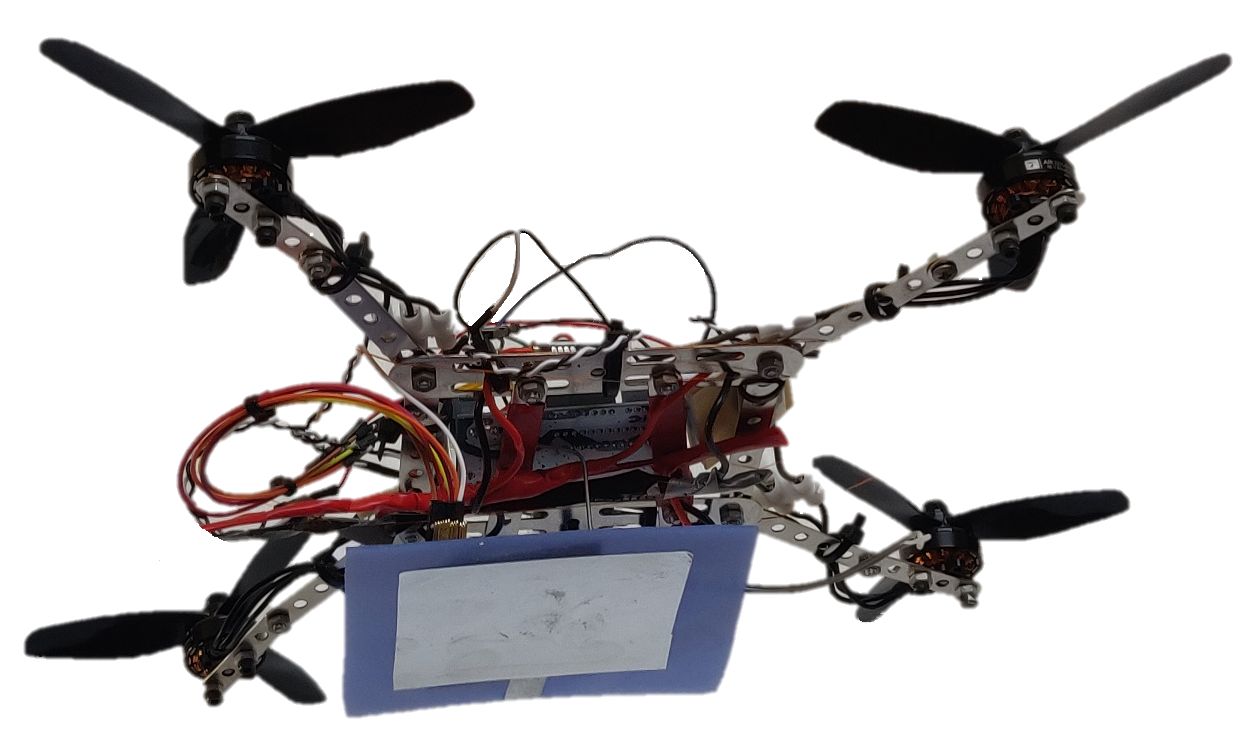
\includegraphics[width=0.9\linewidth]{drone.png}
  \caption{Image of a microstrip patch antenna attached to the bottom of a \gls{UAV}. }
  \label{fig:exampleDrone}
\end{figure}

\section{Methodology}
\subsection{Electromagnetic Exposure}
\subsubsection{Total Electromagnetic Exposure}
The total whole body SAR ($SAR^{wb,total}_{10g}$) of a user can be calculated by a simple sum of individual SAR values from the different sources
and is based on \cite{J17_kuehn2019modelling}. This formula assumes that the users are holding their device next to their ear and therefore 
investigates localized \gls{SAR} for head and torso area.
However for this case, this would result into incorrect conclusions since 
the position of the device relative to the user is unknown. 
The position of the phone can be next to the head but also in front of the user.
The induced electromagnetic radiation will therefore be expressed in function of the entire body.

\begin{equation} 
\begin{aligned}
SAR^{wb,total}_{10g} = SAR^{wb,myUE}_{10g} +  SAR^{wb,myUABS}_{10g} \\
+ SAR^{wb,otherUE}_{10g} + SAR^{wb,otherUABSs}_{10g}
\end{aligned}
\label{eq:overallSARwb}
\end{equation}

The first parameter, $SAR^{wb,myUE}_{10g}$, indicates the absorbed electromagnetic radiation by the whole body originating from the user's own device. Despite that the 
\gls{UL} radiation is destined for the serving \gls{UABS}, a portion of that radiation is directly absorbed by its user, due to the omnidirectional nature of the mobile's antenna.
The second parameter, $SAR^{wb,myUABS}_{10g}$, represents the \gls{DL} radiation caused by the \gls{UABS} that is serving the user.
As the third parameter, we have the $SAR^{wb,otherUE}_{10g}$ which is radiation caused by other people's devices. The radiation of these devices is once again 
destined for a specific \gls{UABS} but again, a portion of that \gls{UL} radiation will also be absorbed by our user.
Finally, $SAR^{wb,otherUABSs}_{10g}$ represents the \gls{DL} radiation by the other \gls{UABS}s to which our user is exposed to but not served by.
An illustration is given in figure \ref{fig:networkIllustration}.
The green arrow stands for near-field radiation, the others represent far-field radiation.

\begin{figure}[h!]
\centering
  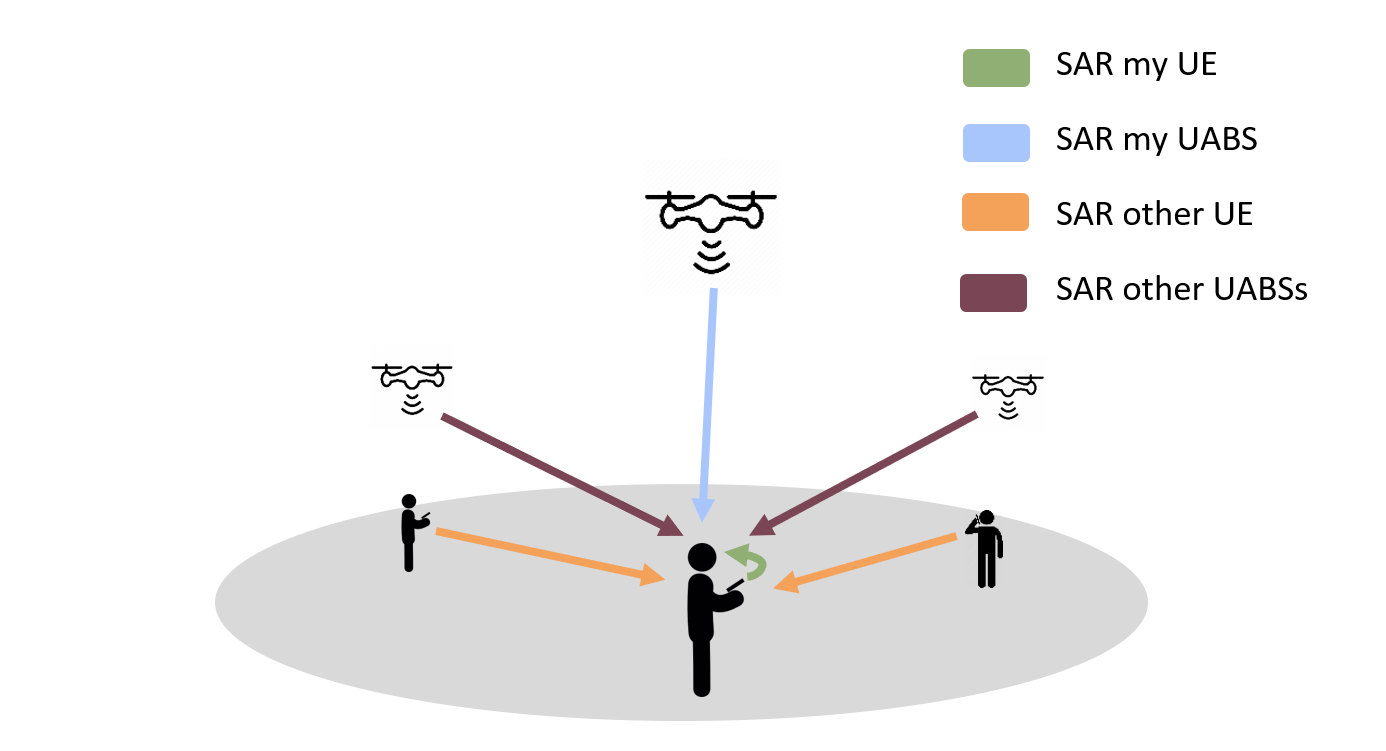
\includegraphics[width=\linewidth]{networkIllustrationSARSources.png}
  \caption{Illustration of the network that shows how the average user (here shown in the center) is influenced by different types of sources. }
  \label{fig:networkIllustration}
\end{figure}

\subsubsection{Electromagnetic Radiation from a Single Source}
\label{sec:calculatingexposure}

In order to find the total electromagnetic radiation to which a user is exposed, 
the electromagnetic radiation from each sources needs to be calculated first.
This is done with formula \ref{eq:singleexposure} which applies to all sources in the far-field.
This includes all \gls{UABS}s and all \gls{UE}  belonging to other people.
The exposure $E$ of a single user $u$ from a single radiator $i$ can be calculated
as follows.

\begin{equation}
E_i(u) [V/m] = 10^{\frac{RRP(u)[dBm] - 43.15 + 20*\log(f [MHz])- PL(u) [dB]}{20}}
\label{eq:singleexposure}
\end{equation}

Calculating the real radiation power (RRP) for a certain user $u$, requires first the \gls{EIRP}-value to be calculated  \cite{J6_originalExposureFormula,J1}.
This is achieved by adding the transmission power $P_{tx}$ to the transmitter gain $G_t$ and thereafter subtracting the feeder loss $L_t$.
This formula needs to be expanded to also account for attenuation from the used antenna. This value depends on the angle
between this user and the antenna's main beam. The attenuation from an \gls{isotropicradiator} is always zero. This leads to the following formula.

\begin{equation}
\begin{aligned}
RRP [dBm] = P_{tx} [dBm] + G_t [dBi]- L_t [dB]\\
     - attenuation(u) [dB]
\end{aligned}
\label{eq:eirp}
\end{equation}
The used frequency in formula \ref{eq:singleexposure} is denoted as $f$ and is expressed in MHz. Since \gls{LTE} is used, this value will be 2600 MHz.

At last, formula \ref{eq:singleexposure} requires the path loss $PL$. In order to calculate this, an appropriate propagation model ---of which several exist--- is required.
The Walfish-Ikegami model is used since it performs well for femtocell networks in urban areas \cite{J2}. %optioneel kan je hier dezelfde bron gebruiken als dat ze in thesis van de vorige gebruikten. Bron nummer 32
%It consists of two formulas depending on whether a free LOS between the user and the base station exists or not. Both formulas expect a distance in kilometre. %bron?

\subsubsection{Combining Exposure}
The total electromagnetic exposure $E_{tot}$, in a certain spot, originating from different sources can be calculated with formula \ref{eq:totalexposure}. $E_i$ stands for 
the electromagnetic exposure from source $i$ and
$n$ stands for all far-field radiators of a certain category which will either be UABSs or UE from other people.
$E_{tot}$ will be calculated for each location where a user is positioned.  
\begin{equation}
E_{tot} [V/m] = \sqrt{\sum_{i=1}^{n} (E_i [V/m]) ^2}
\label{eq:totalexposure}
\end{equation}

\subsubsection{Converting electromagnetic radiation into SAR-values}
Formula \ref{eq:overallSARwb} expects that the radiation is expressed in whole body \gls{SAR}-values.
To make this calculation possible, a distinction has to be made between near-field \gls{SAR}
($SAR^{wb,nf}$) and far-field \gls{SAR} ($SAR^{wb,ff}$). $SAR^{wb,myUE}_{10g}$ is a form of near-field radiation, 
all the other types are far-field radiation.
%$SAR^{wb,my\_UABS}_{10g}$, $SAR^{wb,other\_UE}_{10g}$ and $SAR^{wb,other\_UABSs}_{10g}$ are forms 
%of far-field radiation while $SAR^{wb,my\_UABS}_{10g}$ is a form of near-field radiation.

Converting the electromagnetic radiation is done with a conversion factor which is based 
on Duke of the Virtual Family. Duke is a 34-year old male with a weight of 72 kg, a height of 1.74 m and BMI of 23.1 kg/m \cite{J22_plets2015joint}. 
Research shows that the conversion factor for WiFi in the far-field is $0.0028 \frac{W/kg}{W/m^2}$
and 0.0070 $\frac{W/kg}{W}$ for the near-field \cite{J22_plets2015joint}.
Since WiFi, at a frequency of 2400 MHz,
is very close to \gls{LTE}, at 2600 MHz, it is assumed in \cite{J22_plets2015joint} that this value is also applicable for \gls{LTE}.
Calculating \gls{SAR} from far-field radiation is done as follows:

\begin{equation}
S [W/m^2]= \frac{(E_{tot} [V/m])^2}{337}
\label{eq:flux}
\end{equation}

\begin{equation}
SAR^{wb,ff}_{10g} [W/kg]= S [W/m^2]* 0.0028 \left[\frac{W/kg}{W/m^2}\right]
\label{eq:DLconversion}
\end{equation}

The constant in equation \ref{eq:DLconversion} converts the \gls{power flux density} $S$ to the required $SAR^{ff,wb}_{10g}$.
To make this possible, the electromagnetic radiation
from formula \ref{eq:totalexposure} should first be converted to the  \gls{power flux density} with formula 
\ref{eq:flux}.

The SAR caused by near-field radiation is calculated by multiplying the constant with the used transmission
power $P_{tx}$ of the \gls{UE} which results in the following formula:

\begin{equation} 
SAR^{wb,nf}_{10g} \left[\frac{W}{kg}\right] = 0.0070 \left[\frac{W/kg}{W}\right] * P_{tx} [W]
\label{eq:ulToSar}
\end{equation}

The power of the \gls{UE} can be calculated using equation \ref{eq:powerUE} \cite{J22_plets2015joint}.
\begin{multline}
P_{tx}^{UE} = min \big\{P_{max} [dBm] , \\
 P_{pusch} [dBm] + \alpha * PL [dB] + 10log(M) + \sigma \big\}
 \label{eq:powerUE}
\end{multline}

$P_{max}$ is the maximum allowed transmission power by \gls{UE} for LTE, defined at 23 dBm. 
However, this is the worst case and the actual used power is usually much lower thanks to power control.
$P_{pusch}$ is the required received power at the
\gls{UABS} and will here be -120 dBm. 
$\alpha$ is the path loss compensation factor set to one which means full compensation \cite{J32,J33}.
For the 20-MHz channel used in this paper, $M$ will be set to 100 
and $\sigma$,  as the correction factor, is set to zero \cite{J22_plets2015joint,J32}.


\subsection{Microstrip Patch antenna}
A microstrip patch antenna is chosen because it allows easy production but more important, it has a low weight 
and has a thin profile causing it to be very aerodynamic which is useful when attaching it to a drone \cite{J13_microstripadvantages}.

The dimensions of the antenna depend on the frequency it is operating at and the characteristics of the used substrate.
The antenna will be radiating at a centre frequency $f_0$ of 2.6 GHz. Each substrate has a dielectric constant $\epsilon_r$ representing 
the permittivity of the substrate that depends on the used material.
Substrates with a high dielectric constant and low height 
reduce the dimensions of the antenna
while a lower dielectric constant with a high height improves the performance of the antenna \cite{J14_antennadesign,J15_antennadesign}. 
In this research, a substrate like glass 
is chosen because of the higher dielectric constant of $\epsilon_r = 4.4$ compared to materials like Teflon with only a dielectric 
constant of $\epsilon_r = 2.2$ \cite{J14_antennadesign}. 
Doing this in combination with an antenna height of 2.87 mm will decrease the dimensions of the entire antenna surface.
This comes in handy since \gls{UAV}s only have limited space available.
\newline
\newline
\begin{table}[h!]
\centering
\begin{tabular}{|l|c|l|}
\hline
 Description            & Symbol          & Value         \\    \hline
 Center frequency       & $f_0$           & 2600 MHz       \\ 
 Dielectric constant    & $\epsilon_r$    & 4.4         \\ 
 Height of the substrate & $h$             & 0.00287 m    \\ \hline
\end{tabular}
\caption{Overview of configuration parameters.}
\label{table:antennaparas}
\end{table}

The dimensions of the radiating patch can be calculated with the formulas from \cite{J14_antennadesign,J15_antennadesign}.
Doing so will result in a radiating patch of 35.09 mm by 26.55 mm and a groundplane of at least 52.40 mm by 43.80 mm.
The microstrip patch antenna as illustrated in fig. \ref{fig:basicpatchantenna} will result in the radiation pattern of fig. \ref{fig:radpattern}.

\begin{figure}[h!]
\centering
  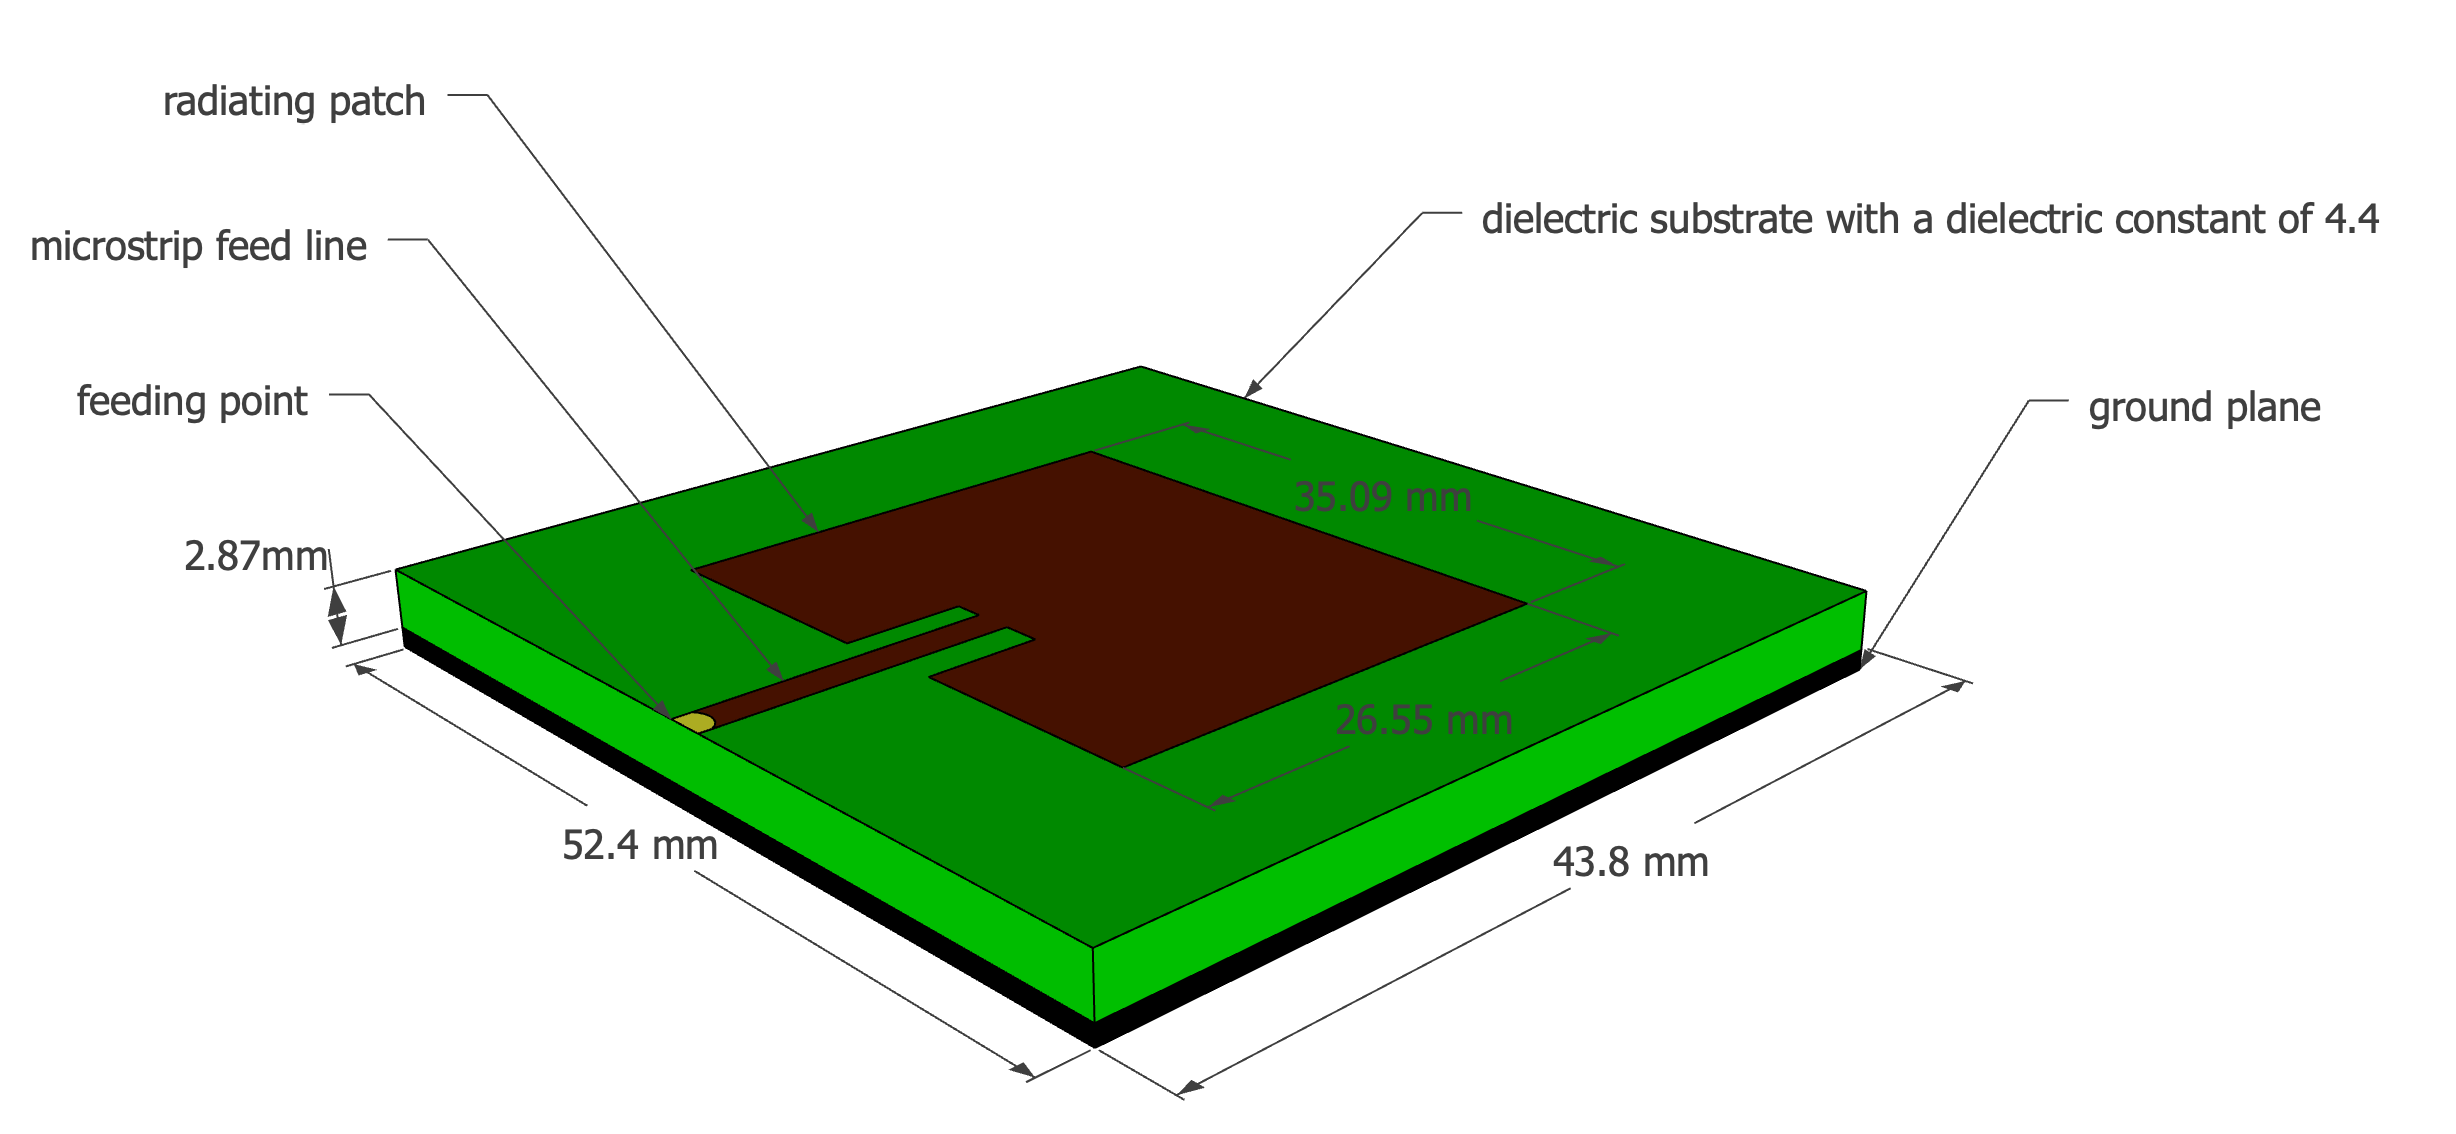
\includegraphics[width=\linewidth]{MicrostripAntenna.png}
  \caption{Design of the microstrip patch antenna.}
  \label{fig:basicpatchantenna}
\end{figure}

\begin{figure}[!htb]
\subfloat[E-plane]{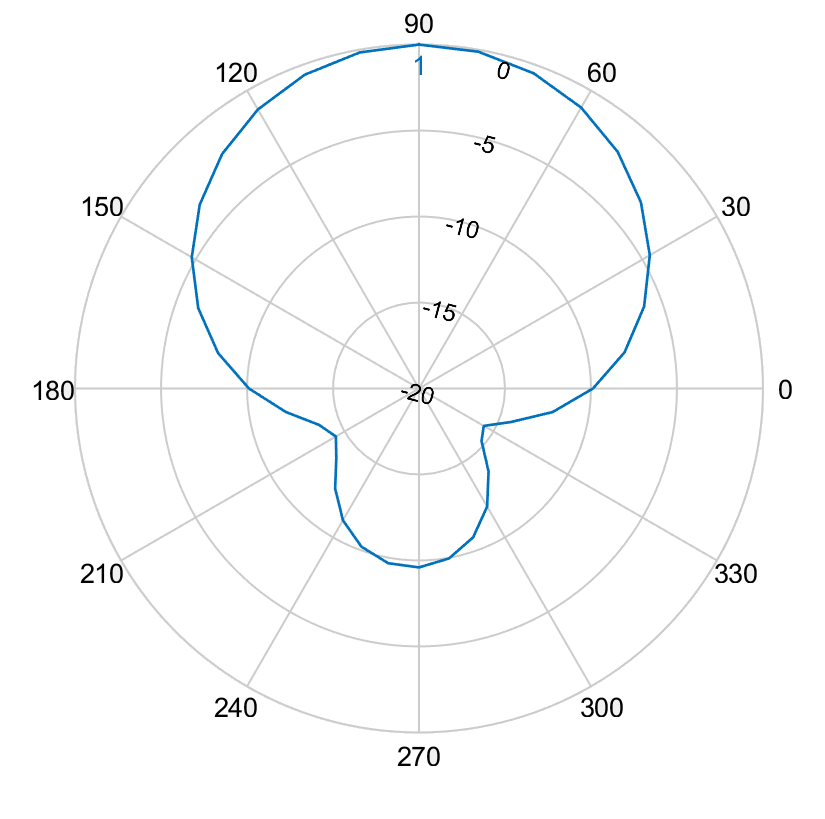
\includegraphics[width=0.49\linewidth]{pattern2/ep.png}}
\hfill
\subfloat[H-plane]{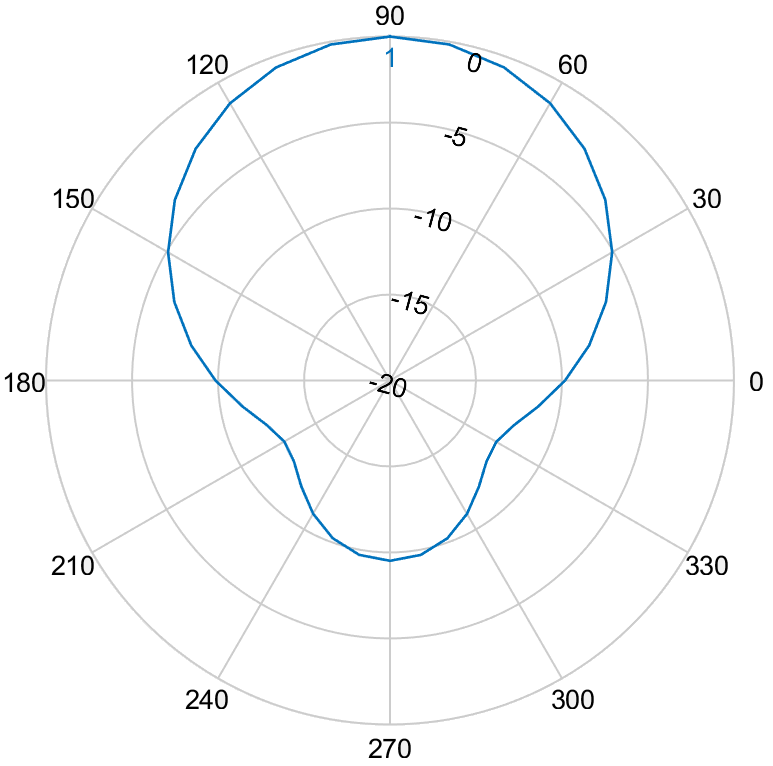
\includegraphics[width=0.49\linewidth]{pattern2/hp.png}}
  \caption{Radiation patterns generated by the used microstrip patch antenna.}
\label{fig:radpattern}
\end{figure}

\subsection{Optimizing the network}
Deruyck et al. discusses in \cite{J1} how a terrestrial  telecommunication network either can be optimized towards electromagnetic 
exposure of an individual or towards power consumption of the entire network. 
However, an increasing transmission power of an antenna comes with an increasing electromagnetic exposure. This is not the case considering
both values for an entire network. In fact, the authors from \cite{J1}  prove that both become inversely equivalent.
The reason why the network behaves like this is because it is often cheaper to increase the exposure of an already active base station 
than activating a new one. 
This leads to the following fitness function which is based on \cite{J1}.

\begin{equation} 
f = w * \left(1 - \frac{E_m}{E_{max}}\right) + (1 - w)*\left(1 - \frac{P}{P_{max}}\right) * 100
\label{eq:fitnessfunction}
\end{equation}

Formula \ref{eq:fitnessfunction} returns a fitness value which represents the performance of the entire network. 
$w$ is the importance factor of electromagnetic exposure ranging from 0 to 1, boundaries included. A $w$ set to 0 means that electromagnetic 
exposure is not important. Such network will therefore be called a \gls{PwrC Opt} network. 
Likewise, a $w$ set to 1 means that minimizing exposure is top priority and will result in an \gls{Exp Opt} network. $P_{max}$ is the power consumption of all UABSs, 
both active and inactive, when radiating at the highest level possible 
while $P$ is the effective power used by the current designed network. 
This will be the power required for the flying \gls{UAV}s themselves and their antennae.
$E_m$ will be the weighted exposure of the average user for the current designed network and $E_{max}$ the weighted average of the electromagnetic exposure when all antennae 
are at their highest power level.

When optimizing the network, it is not only important to consider the average exposure of all users, but also to limit high extremes \cite{J1}. A weighted average 
will be used not only considering the median but also the 95 percentile from all users' \gls{DL} exposure using formula \ref{eq:em}. 
Since both values are considered to have equal importance, the weight factors $w_1$ and $w_2$ will both have an equal importance of 50\%. 

\begin{equation} 
E_m = \frac{w_1 * E_{50} + w_2 * E_{95}}{w_1 + w_2}
\label{eq:em}
\end{equation}


\subsection{Simulation Tool}

\subsubsection{Main Algorithm}
First, a description of the area has to be provided to the tool. This is done with so-called shape-files.
These  files contain a complete description about the shape of the buildings. Thereafter, users are uniformly
distributed over the area and a temporary \gls{UABS} is positioned above each user. Now, the decision algorithm
needs to decide which of these \gls{UABS}s can actually remain and how hard each one should be radiating. Once the 
decision algorithm is done, the tool checks whether the number of online \gls{UABS}s does not acceed the capacity of 
the facility where the \gls{UABS}s are stored. If this is the case, the \gls{UABS}s covering the least amount of users 
will be removed.

\subsubsection{Decision Algorithm}

Solving the network is done by the decision algorithm and starts by calculating the path loss between all users and between users and \gls{UABS}s.
Thereafter, the algorithm iterates over each user and tries to connect that user to each \gls{UABS}. This connection is not always possible. A \gls{UABS} might be saturated with users and 
will not be able to cover yet another one or maybe the user is so far away that in order to cover that user, the \gls{UABS} would have to exceed its maximum allowed input power.
If however a connection is possible, the user will be connected to that \gls{UABS} and the fitness function (eq. \ref{eq:fitnessfunction} is applied. 
This is repeated for each \gls{UABS}. Only the connection which results in the best fitness value for the entire network will be used.
Doing so will make sure that, given the currently designed network, the user is optimized. In other words, each user is optimized and 
not the entire network. It is however assumed that the average network will be optimized as well.
 Thereafter, the tool shifts to the next user. 
When the last user has been processed, the network is fully designed for an unlimited number of \gls{UAV}s and the result is returned to the main algorithm for further processing.
The flowchart of this algorithm is given in figure \ref{fig:decisionAlgoFlowChart}.

\begin{figure}[h!]
\centering
  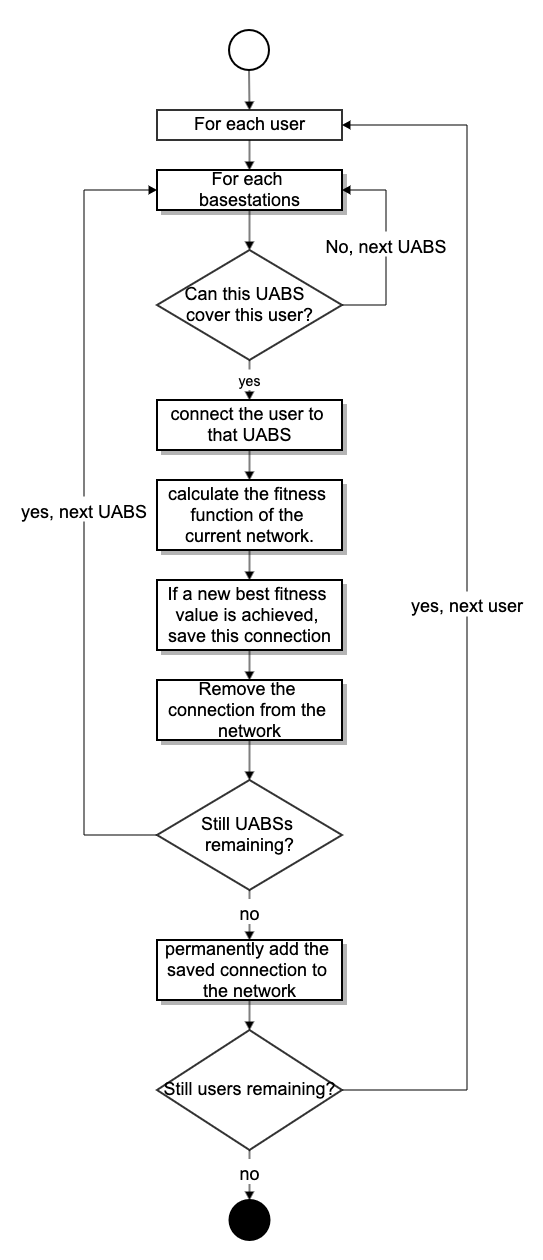
\includegraphics[height=0.8\textheight]{decisionAlgoFlowChart.png}
  \caption{Flowchart of the decision algorithm.}
  \label{fig:decisionAlgoFlowChart}
\end{figure}

%%%%%%%%%%%%%%%%%%%%%%%%%%%%%%%%%%%%%%%%%%%%%%%%%%%%%%%%%%%%%%%%%%%%%%%%%%%%%%%%%%%%%%%%%%%%%%%%%%%%%%%%%%%%%%%%%%%
\FloatBarrier
\section{Scenarios}
The default configuration is given in table \ref{table:defaultconf} and is always applicable unless mentioned otherwise. 

\begin{table}[!htb]
\centering
\begin{tabular}[t]{ll}
        \toprule
        \multicolumn{2}{l}{\textbf{Broadband cellular network}} \\
        \hline
        \hspace{3mm}  Technology                          & LTE     \\
        \hspace{3mm}  Frequency                           & 2.6 GHz \\
        \hspace{3mm}  Power offset ($P_{pusch}$)            & -120 dBm  \\
        \hspace{3mm}  Path loss compensation ($\alpha$)   & 1  \\
        \hspace{3mm}  Correction value                    & 0 dBm  \\
        \hspace{3mm}  Number of used resource blocks      & 100  \\
        \hline
        \multicolumn{2}{l}{\textbf{Femtocell antenna}} \\
        \hline  
        \hspace{3mm}  Maximum $P_{tx}$                    & 33 dBm   \\
        \hspace{3mm}  antenna  direction                  & downwards   \\ 
        \hspace{3mm}                                      & (az: \ang{0}; el: \ang{90})    \\
        \hspace{3mm}  Gain                                & 4 dBm   \\ 
        \hspace{3mm}  Feeder loss                         & 2 dBm   \\ 
        \hspace{3mm}  Implementation loss                 & 0 dBm   \\
        \hspace{3mm}  radiation pattern                   & EIRP or\\
         \hspace{3mm}                                     & microstrip patch\\
        \hspace{3mm}  Flying altitude                     & 100 m  \\
        \hline
        \multicolumn{2}{l}{\textbf{UAV}} \\
        \hline  
        \hspace{3mm}  UAV power                           & 13.0 A   \\
        \hspace{3mm}  Average UAV speed                   & 12.0 m/s \\
        \hspace{3mm}  Average UAV power usage             & 17.33 Ah    \\
        \hspace{3mm}  UAV battery voltage                 & 22.2 V \\
        \hline
        \multicolumn{2}{l}{\textbf{\acs{UE} Antenna}} \\
        \hline 
        \hspace{3mm} Height                     & 1.5m from the floor       \\ 
        \hspace{3mm} Gain                      & 0 dBm   \\ 
        \hspace{3mm} Feeder loss               & 0 dBm   \\ 
        \hspace{3mm} Radiation pattern         & \acs{EIRP}  \\
        \hspace{3mm} Quantity in network                & 224  \\
        \toprule
\end{tabular}
\caption{Overview of default configuration values.}
\label{table:defaultconf}
\end{table}
 
Three main scenarios will be investigated. 
The first one has only one user and one \gls{UABS} present in the network. 
SAR, electromagnetic exposure, power consumption 
and antenna transmission power are investigated at different flying heights.

In a second scenario, the network is expanded for multiple users while still considering only one \gls{UABS}. 
Two parameters will be evaluated. The first one will be a variable flying height ranging from 
20 to 200 metres with a fixed
number of 224 users. This is the average population size on an usual day at 5 p.m. in Ghent \cite{J2}.
The second evaluated parameter is the number of users ranging from 50 to 600 users
while flying height is set to 100 metres \cite{J2}.
The power consumption, electromagnetic exposure and specific 
absorption rate are investigated for each parameter.

The third scenario is quite similar to the previous scenario. The same two parameters
 are investigated, but now an unlimited number of \gls{UABS}s is available.

Four configurations are considered for each evaluated parameter in each scenario.
There are two possible antennae, namely EIRP 
and microstrip patch antenna, which can both be applied in a \gls{PwrC Opt} network or an \gls{Exp Opt} network.
An overview of the simulation configuration scenarios is presented in figure \ref{fig:fourCasesMatrix}

It is important to note that 
all measured values are strictly limited to the sources mentioned in the previous section and thus only cover data traffic 
between \gls{UE} and \gls{UABS}s. Any other potential sources like backhaul links will not be covered.

\begin{figure}[h!]
\centering
  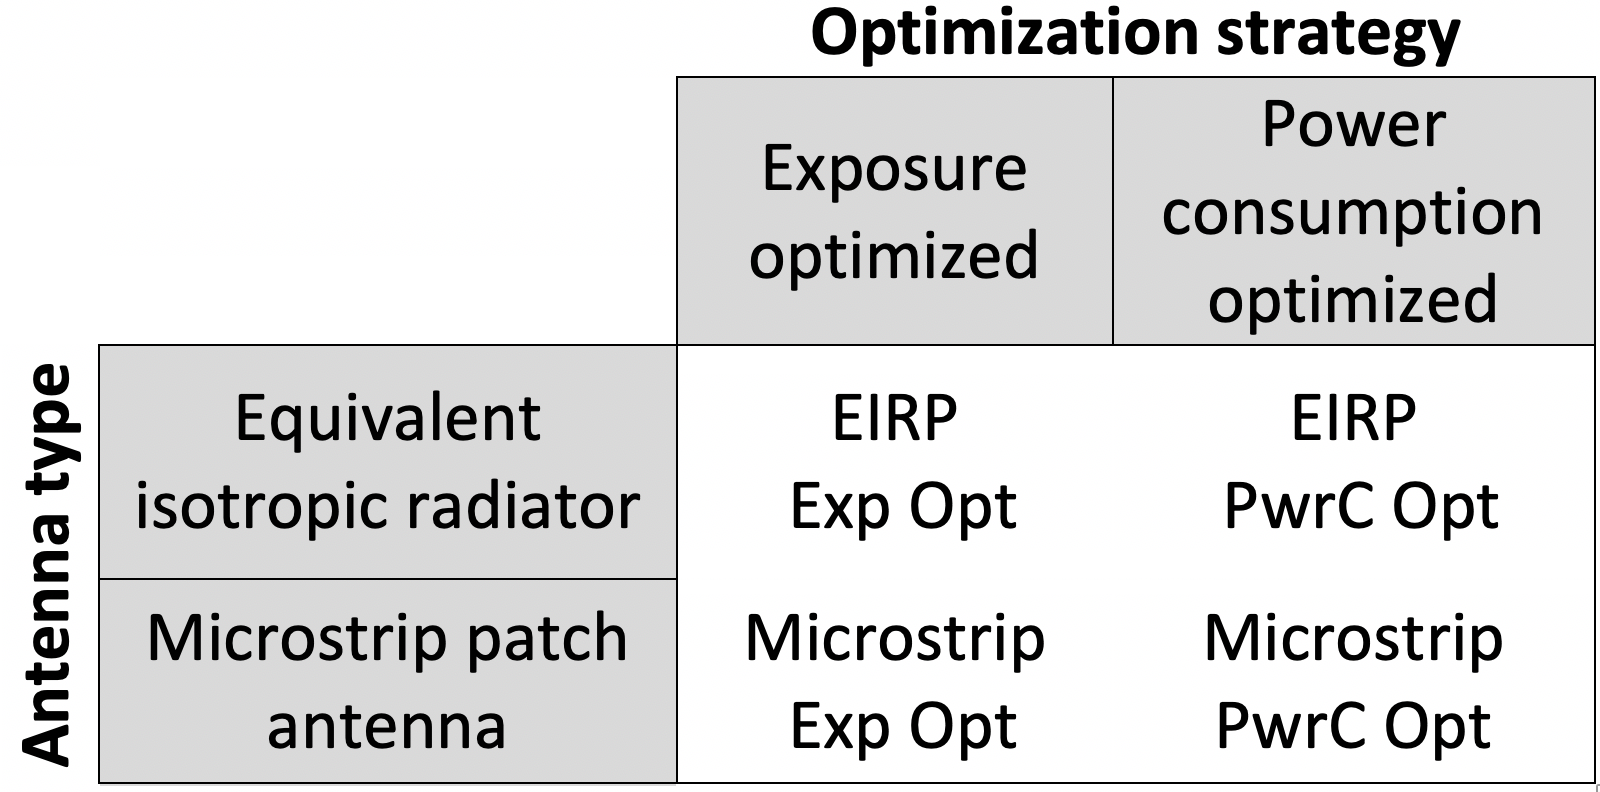
\includegraphics[width=0.7\linewidth]{fourCasesMatrix.png}
  \caption{Matrix with the four possible configurations}
  \label{fig:fourCasesMatrix}
\end{figure}

%%%%%%%%%%%%%%%%%%%%%%%%%%%%%%%% RESULTATEN %%%%%%%%%%%%%%%%%%%%%%%

\section{Results}
Four configurations will be investigated while evaluating two parameter, being the population size and flying height.
The parameters are evaluated for three different scenarios by by monitoring the power consumption, electromagnetic exposure and \gls{SAR}-values.
%This is done for the two considered antennae who can both operate in two optimization strategies, making a total of four possible configurations. The first scenario will cover only one user and one \gls{UABS}. The second scenario has much more users but still only one \gls{UABS}. Finally, the third scenario is similar  to the previous scenario but with unlimited number of \gls{UABS}s available.
The electromagnetic radiation and \gls{SAR} are 
measured for the weighted average user using 
equation \ref{eq:em} with both $w_{1}$ and $w_{2}$ set to 50\%. Each result is averaged over 20 simulations. 

%%%%%%%%%%%%%%%%%%%%%%%%%%%%%%%% S 1  %%%%%%%%%%%%%%%%%%%%%%%
\subsection{One User and One \gls{UABS}}
The  results show that for a varying flying height, a logarithmic relationship exists between the $P_{tx}$ and the flying height. 
This is mainly caused by the logarithmic 
scale in which the decibels of the $P_{tx}$ are expressed.
Each time the flying height becomes too large to cover, the 
$P_{tx}$ increases with one dBm. 
When using the default configuration, with a maximum $P_{tx}$ of 33 dBm,
a \gls{UABS} can fly up to 387 m before losing connection in a free \gls{LOS} scenario.

This scenario is investigated with a microstrip patch antenna using power consumption optimization. 
 However, the chosen optimization strategy does not really matter because the decision 
 algorithm decides which user 
needs to be connected to which \gls{UABS}. Since only one \gls{UABS} is available, both optimization strategies will behave identical.
Further, also the used antenna will not make any difference.
The user is namely positioned in the perfect centre of the main beam where there is 
no attenuation experienced for both antennae.

When investigating this scenario at different flying heights, it is noticed
that the \gls{UL} radiation increases exponentially while 
the \gls{DL} radiation remains constant at $10\ nW/kg$ during the entire time as shown in fig. \ref{fig:s1_fhsar}. The reason that the \gls{DL} radiation
remains constant is because of power control which makes sure that no more power is used than strictly necessary. 
%So at lower flying altitudes, there is less path loss and the \gls{UABS} will therefore reduce the $P_{tx}$. 
We can therefore confirm that the electromagnetic exposure is a constant fraction of power and distance.
The \gls{UL} radiation starts very low at $1\ nW/kg$ but surpasses the \gls{DL} radiation 
around 80 metres.

\begin{figure}[]
\centering
  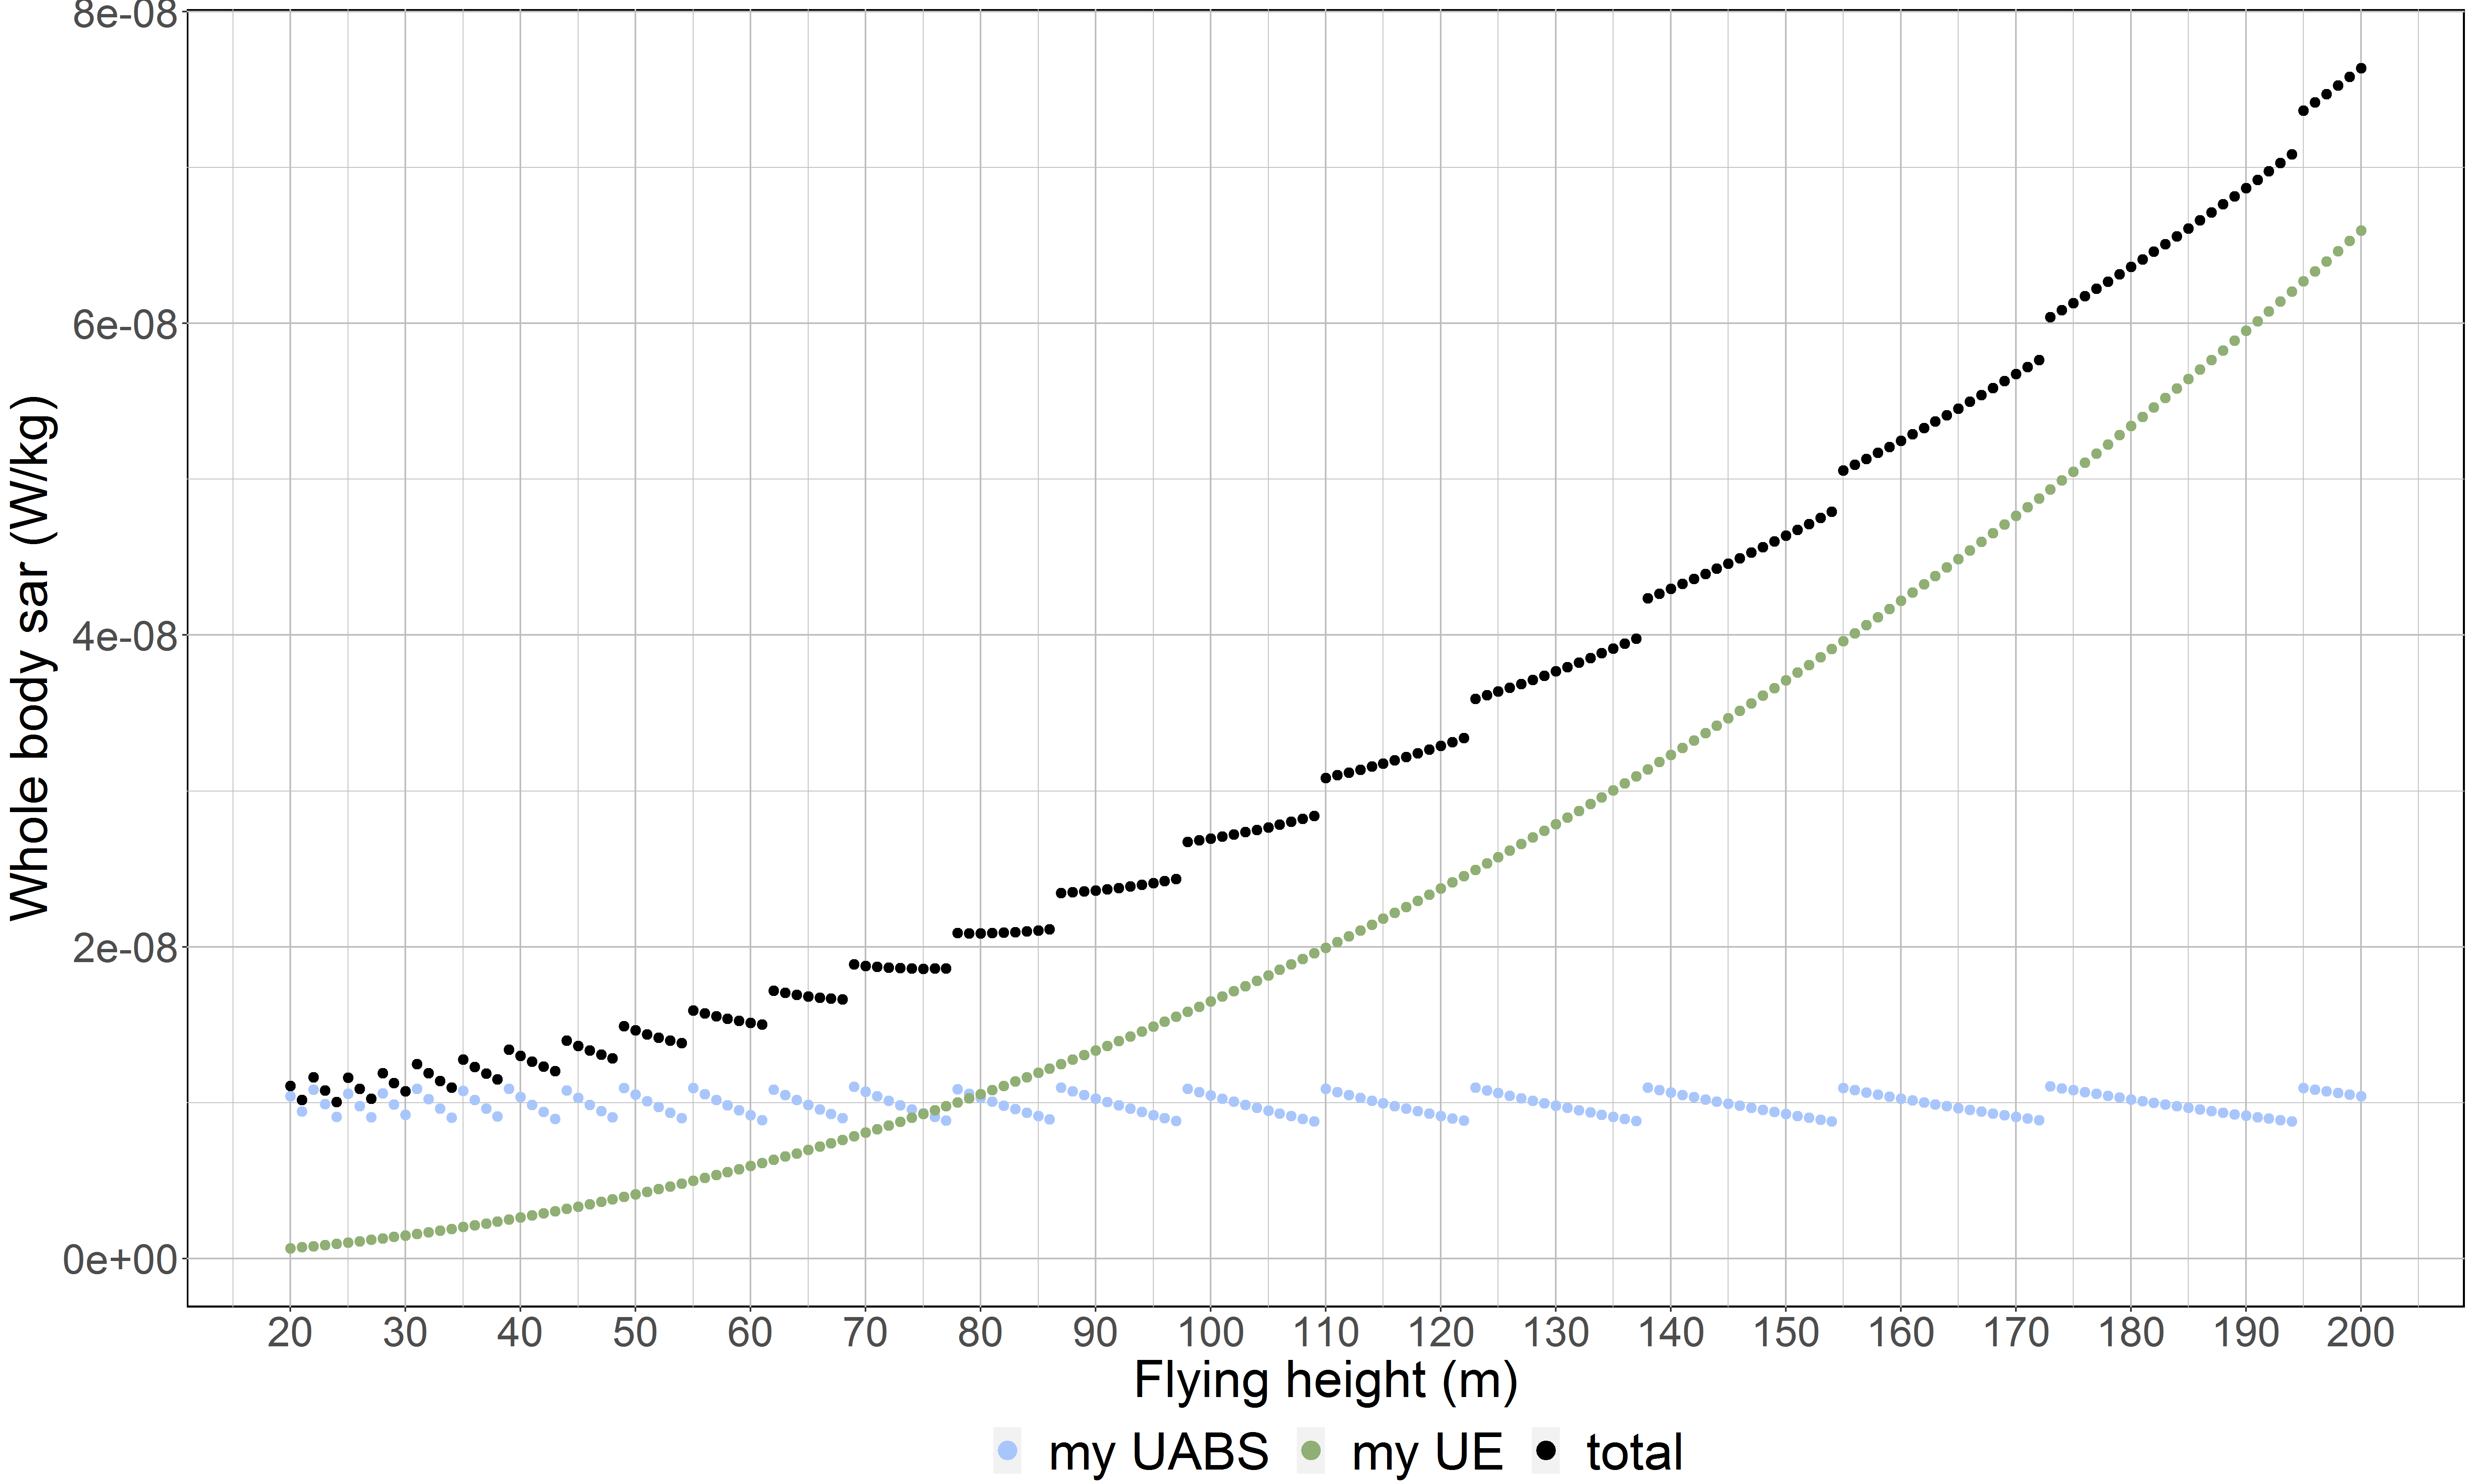
\includegraphics[width=\linewidth]{fhvssar_extendedAbstract.png}
  \caption{This figure shows how SAR values from different sources are influenced by different flying altitudes.}
  \label{fig:s1_fhsar}
\end{figure}

%%%%%%%%%%%%%%%%%%%%%%  S 2  %%%%%%%%%%%%%%%%%%%%%%%%%%%%%%%%%%%%%%

\subsection{Increased Population with one UABS}
\subsubsection{Variable Flying Height}
A \gls{PwrC Opt} network has higher exposure compared to an \gls{Exp Opt} network; a behaviour that was already proven by \cite{J1}. 
However, for this scenario, a \gls{PwrC Opt} network will not necessarily result in a lower power consumption. 
For example, at 100 metres, an \gls{EIRP} \gls{Exp Opt} network exposes the average 
user to $1.5\ mV/m$ less but requires $20\ mW$ more.
To understand this, the behaviour of the deployment tool needs to be understood first. 
A \gls{PwrC Opt} network will result in a few high powered \gls{UABS}s because increasing the input power of an antenna costs 
less than activating a new  \gls{UAV}. Likewise, an \gls{Exp Opt} network 
generates a lot of low powered \gls{UABS}s because the lower the power of the antenna, the lower the exposure. This has the consequence that the cover radius 
is less and therefore requires more \gls{UAV}s which costs more energy.
When only a limited amount of \gls{UABS}s are available, 
like only one in this scenario, the tool will only keep \gls{UABS}s which cover the most users. 
Therefore, the power consumption in a \gls{PwrC Opt} network is often higher. 
\begin{figure}[h!]
  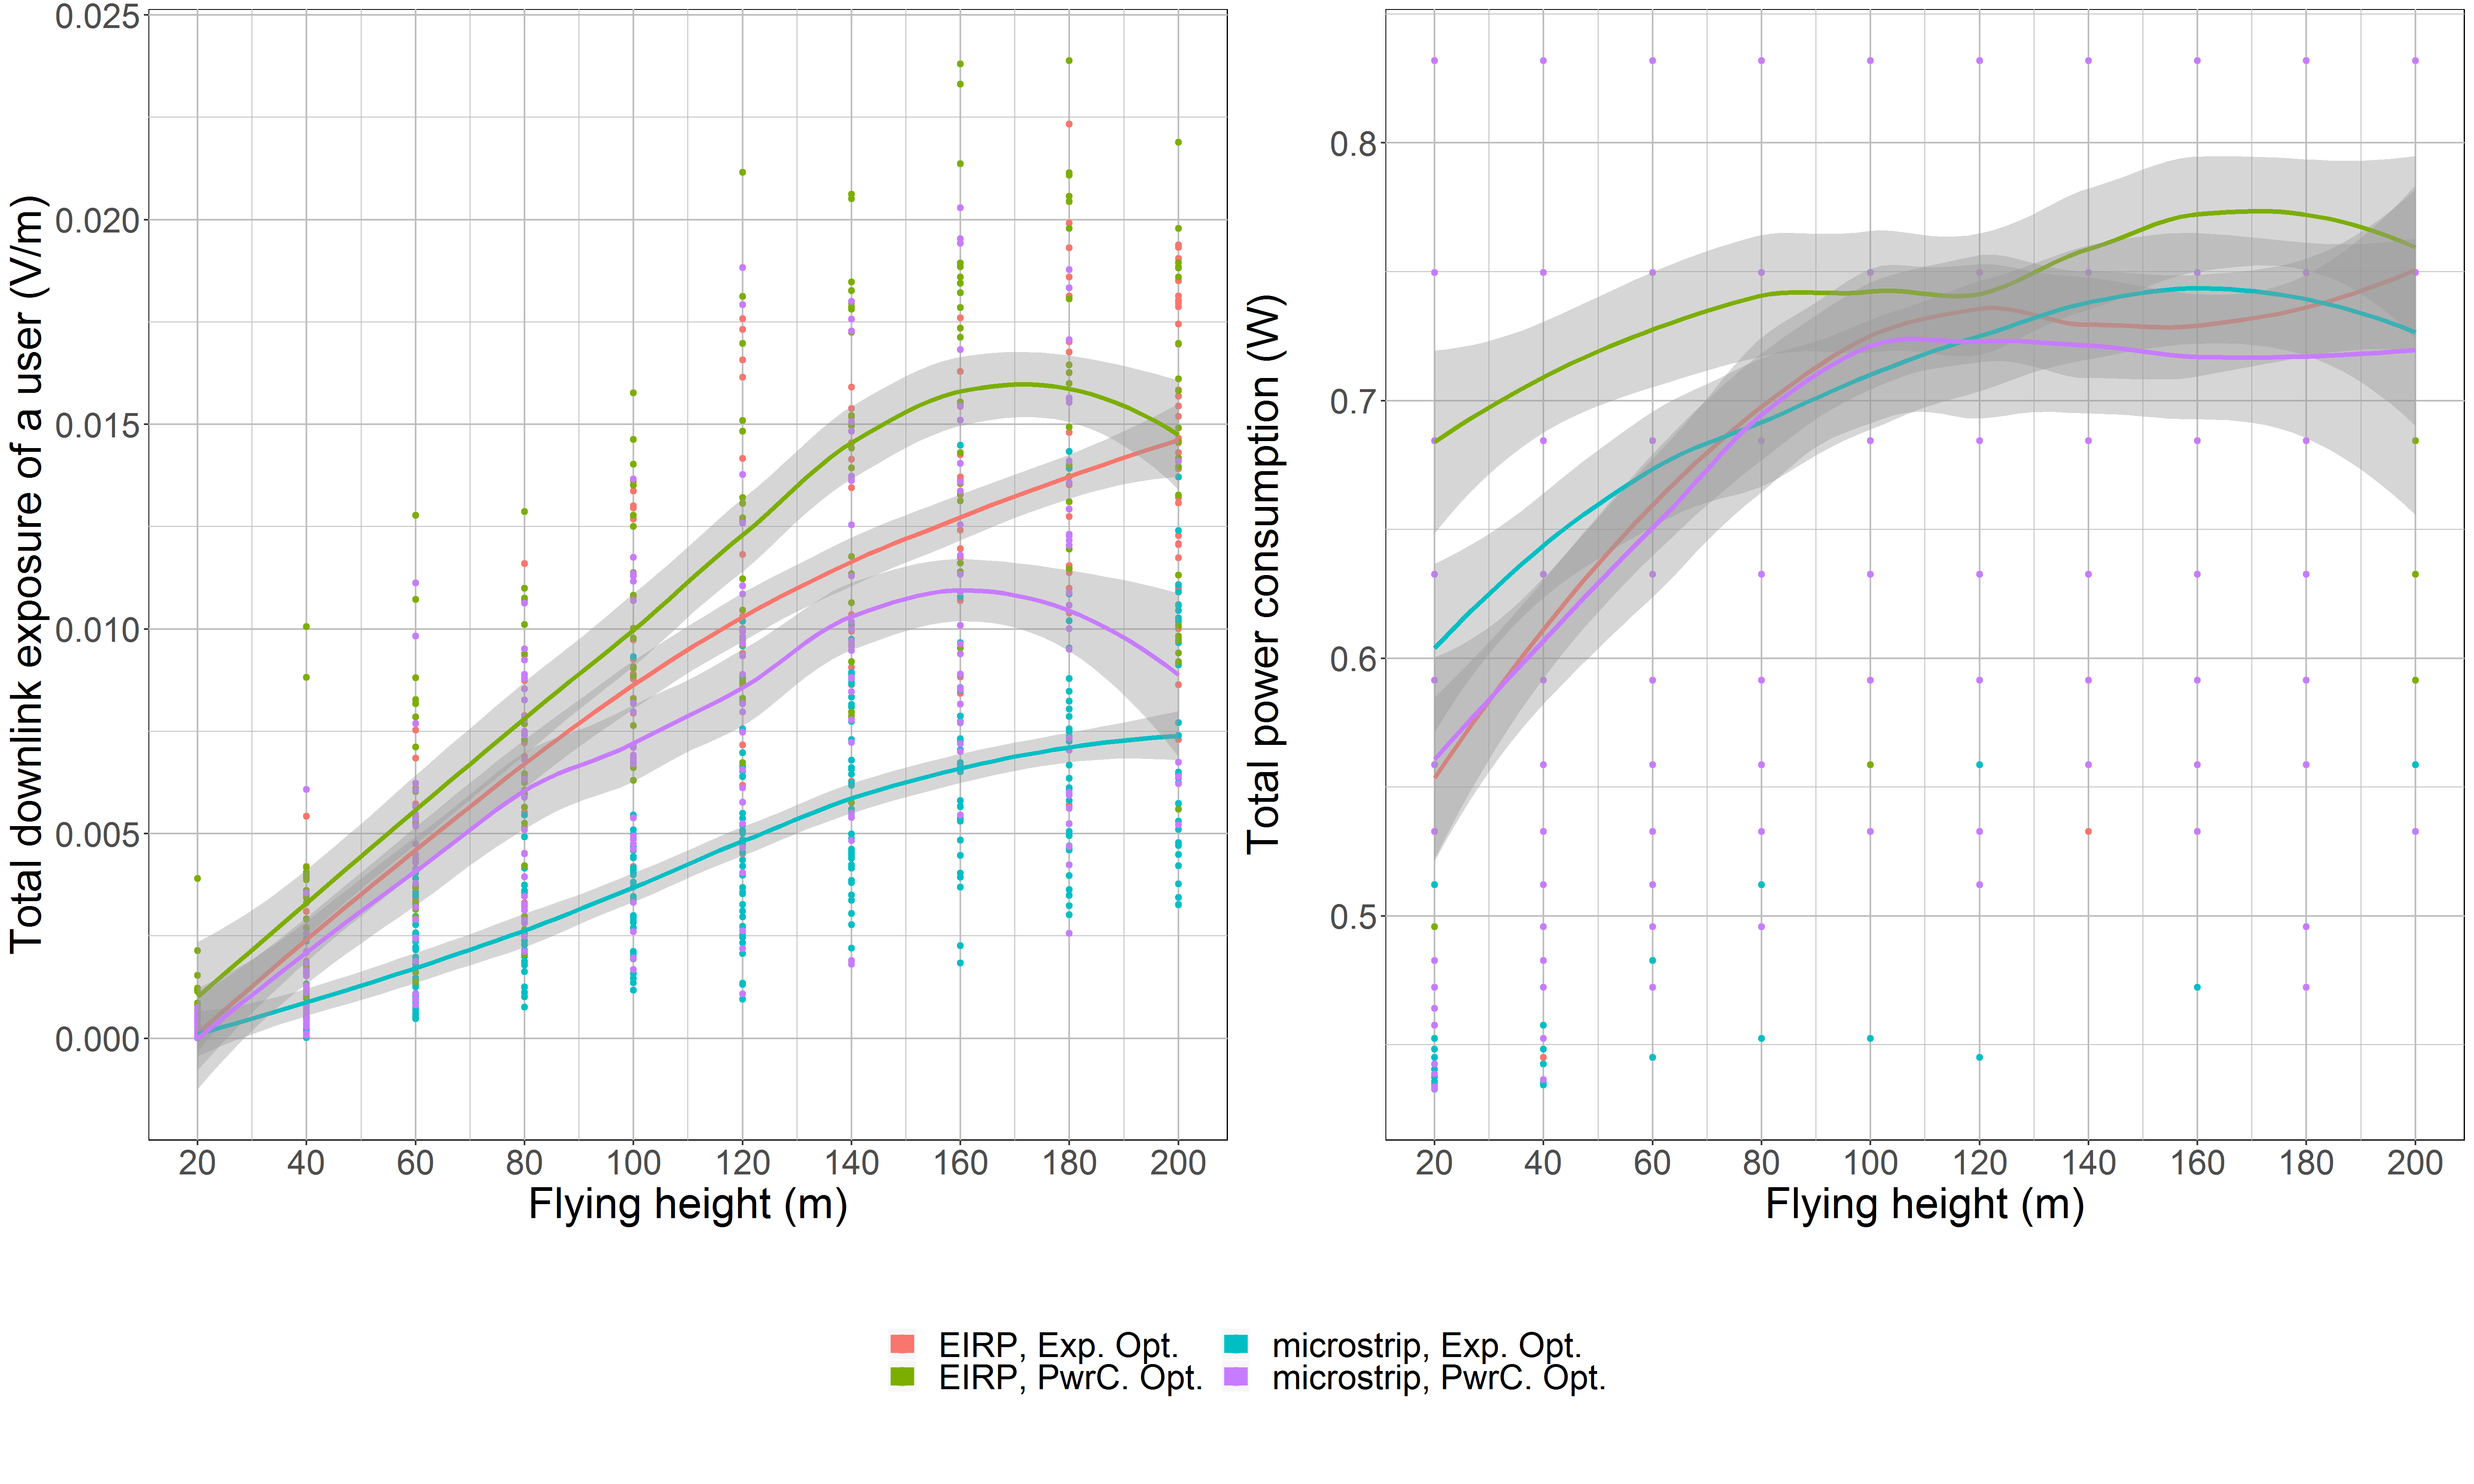
\includegraphics[width=\linewidth]{fhvsdlAndPc_extendedAbstract.png}
  \caption{Fig. (a) show how the flying height influences the downlink electromagnetic radiation of the average user and fig. (b) the
  power consumption of the entire network for the only \acs{UABS} available in the network.}
  \label{fig:s2a_dlAndPc}
\end{figure}

Further, figure \ref{fig:s2a_dlAndPc} also show that the exposure increases with higher flying altitudes
because there is a lower probability of having \gls{NLOS} links by obstructing buildings. This has as consequence that  
more users become covered. 
Increasing the flying height from 20 to 100 metres improves the coverage between 1\% and 2\% for all four configurations.
The increasing electromagnetic radiation is however not unlimited.
A microstrip \gls{PwrC Opt} network is at his highest point  
around 162 metres and an \gls{EIRP} \gls{PwrC Opt} is at his highest at 195 metres.
This decline starts later for exposure optimized networks and is situated outside the investigated flying range.
The decreasing electromagnetic radiation at high flying altitudes is not caused by the obstructing buildings but by the 
distance in general.

Figure \ref{fig:s2shfourSourcesMatrix} shows the whole body $SAR_{10g}$ for the weighted average user, deducted from all electromagnetic sources. 
When investigating the three different sources, we see 
that the $SAR^{myUABS}$ shows the same curve as it did with the electromagnetic exposure 
in figure \ref{fig:s2a_dlAndPc}.a. This is normal behaviour considering that equation \ref{eq:DLconversion} is able of 
converting the \gls{DL} exposure to \gls{SAR} by simply multiplying with a constant.
During the entire time is $SAR^{myUABS}$ the most dominant factor followed by 
 the near-field radiation from the user's own device.
The far-field radiation from other \gls{UE} barely has influence. 
As an illustration, when the \gls{UABS} flies at 140 metres, the average user in an \gls{EIRP} \gls{PwrC Opt} network will 
experience around  2.1 $nW/kg$ from the \gls{UABS} and around 0.2 $nW/kg$ from his own device.
The exposure from other \gls{UE} can be neglected with 0.03 $pW/kg$. A low but plausible value considering that most 
\gls{UE} are not radiating anything since they are uncovered.

\begin{figure}[h!]
\centering
  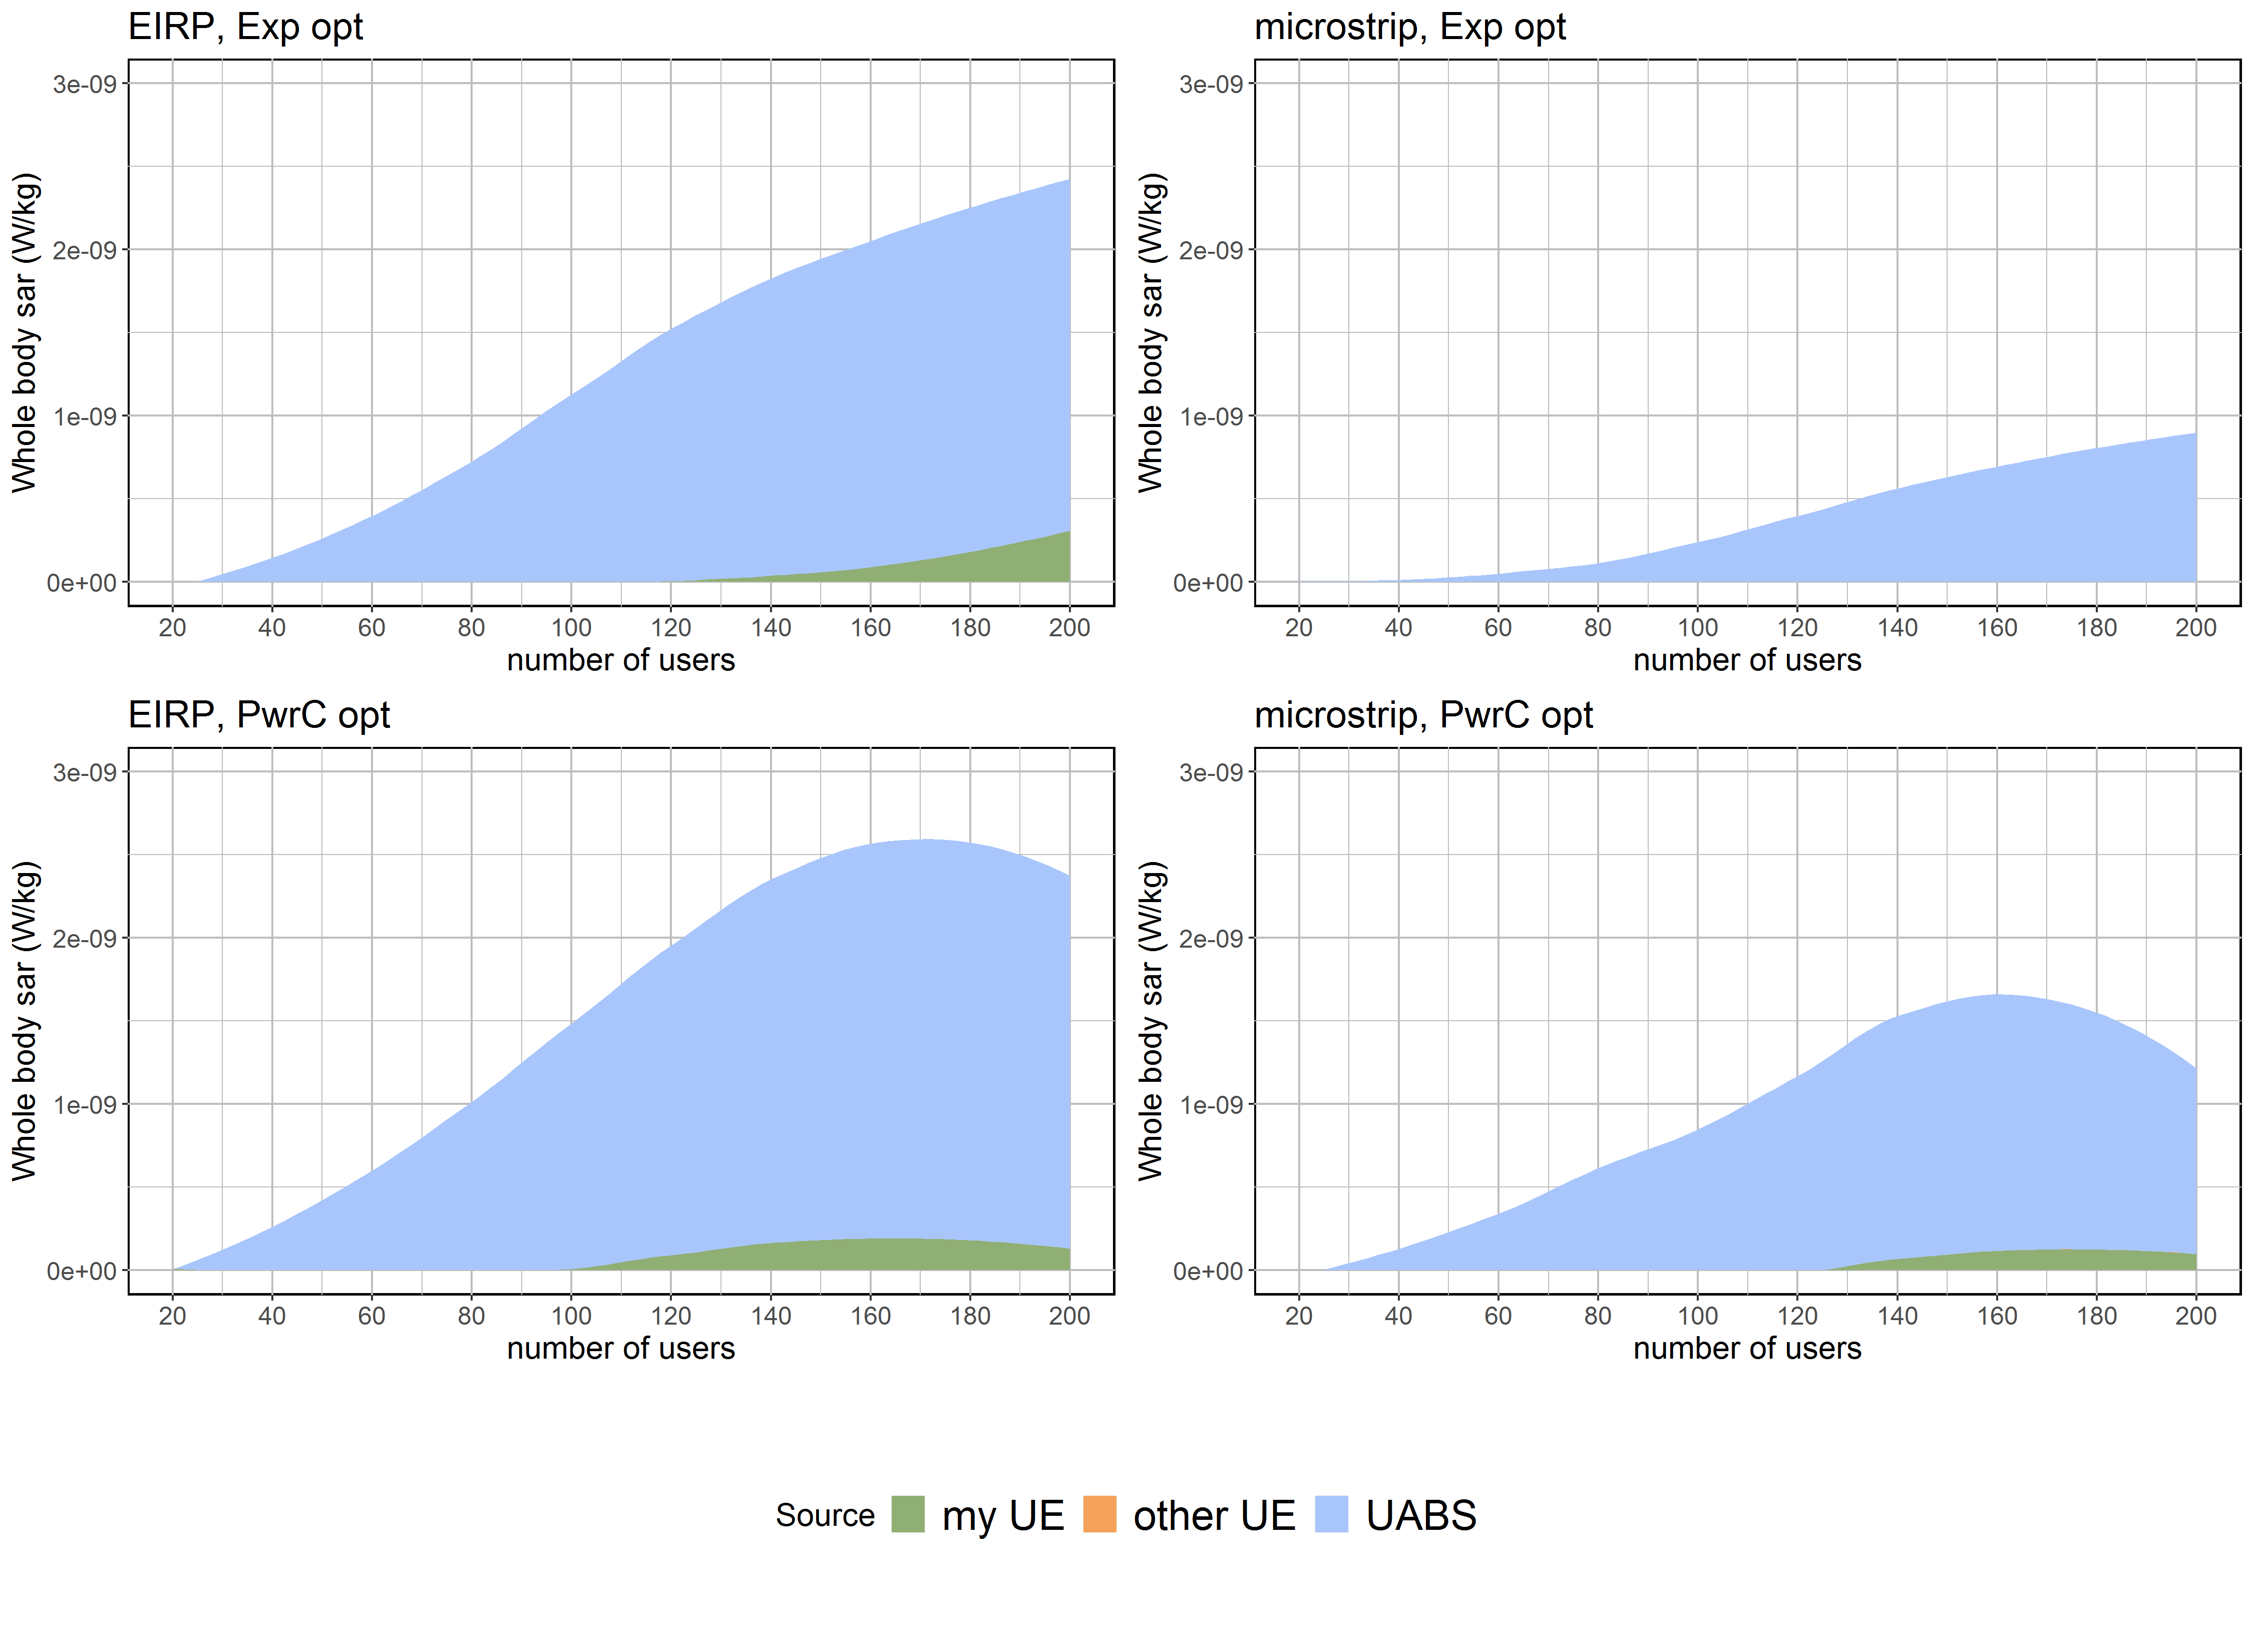
\includegraphics[width=\linewidth]{s2/fhFourSources.png}
  \caption{Influence of the flying height for each considered configuration.
  %Each figure shows how with a certain configuration and shows how the \acs{SAR} from   different sources are influenced by an increasing flying height.
  }
  \label{fig:s2shfourSourcesMatrix}
\end{figure}

\FloatBarrier
\subsubsection{Variable Number of Users}
The number of covered users increases linearly compared to the number of users present in the network as shown in figure 
\ref{fig:s2uvsnumcovusers}.b. It illustrates how an \gls{isotropicradiator} is able to reach more users 
compared to a microstrip patch antenna. Just like an power consumption optimized network 
is able to reach more users than an exposure optimized network.
\begin{figure}[h!]
  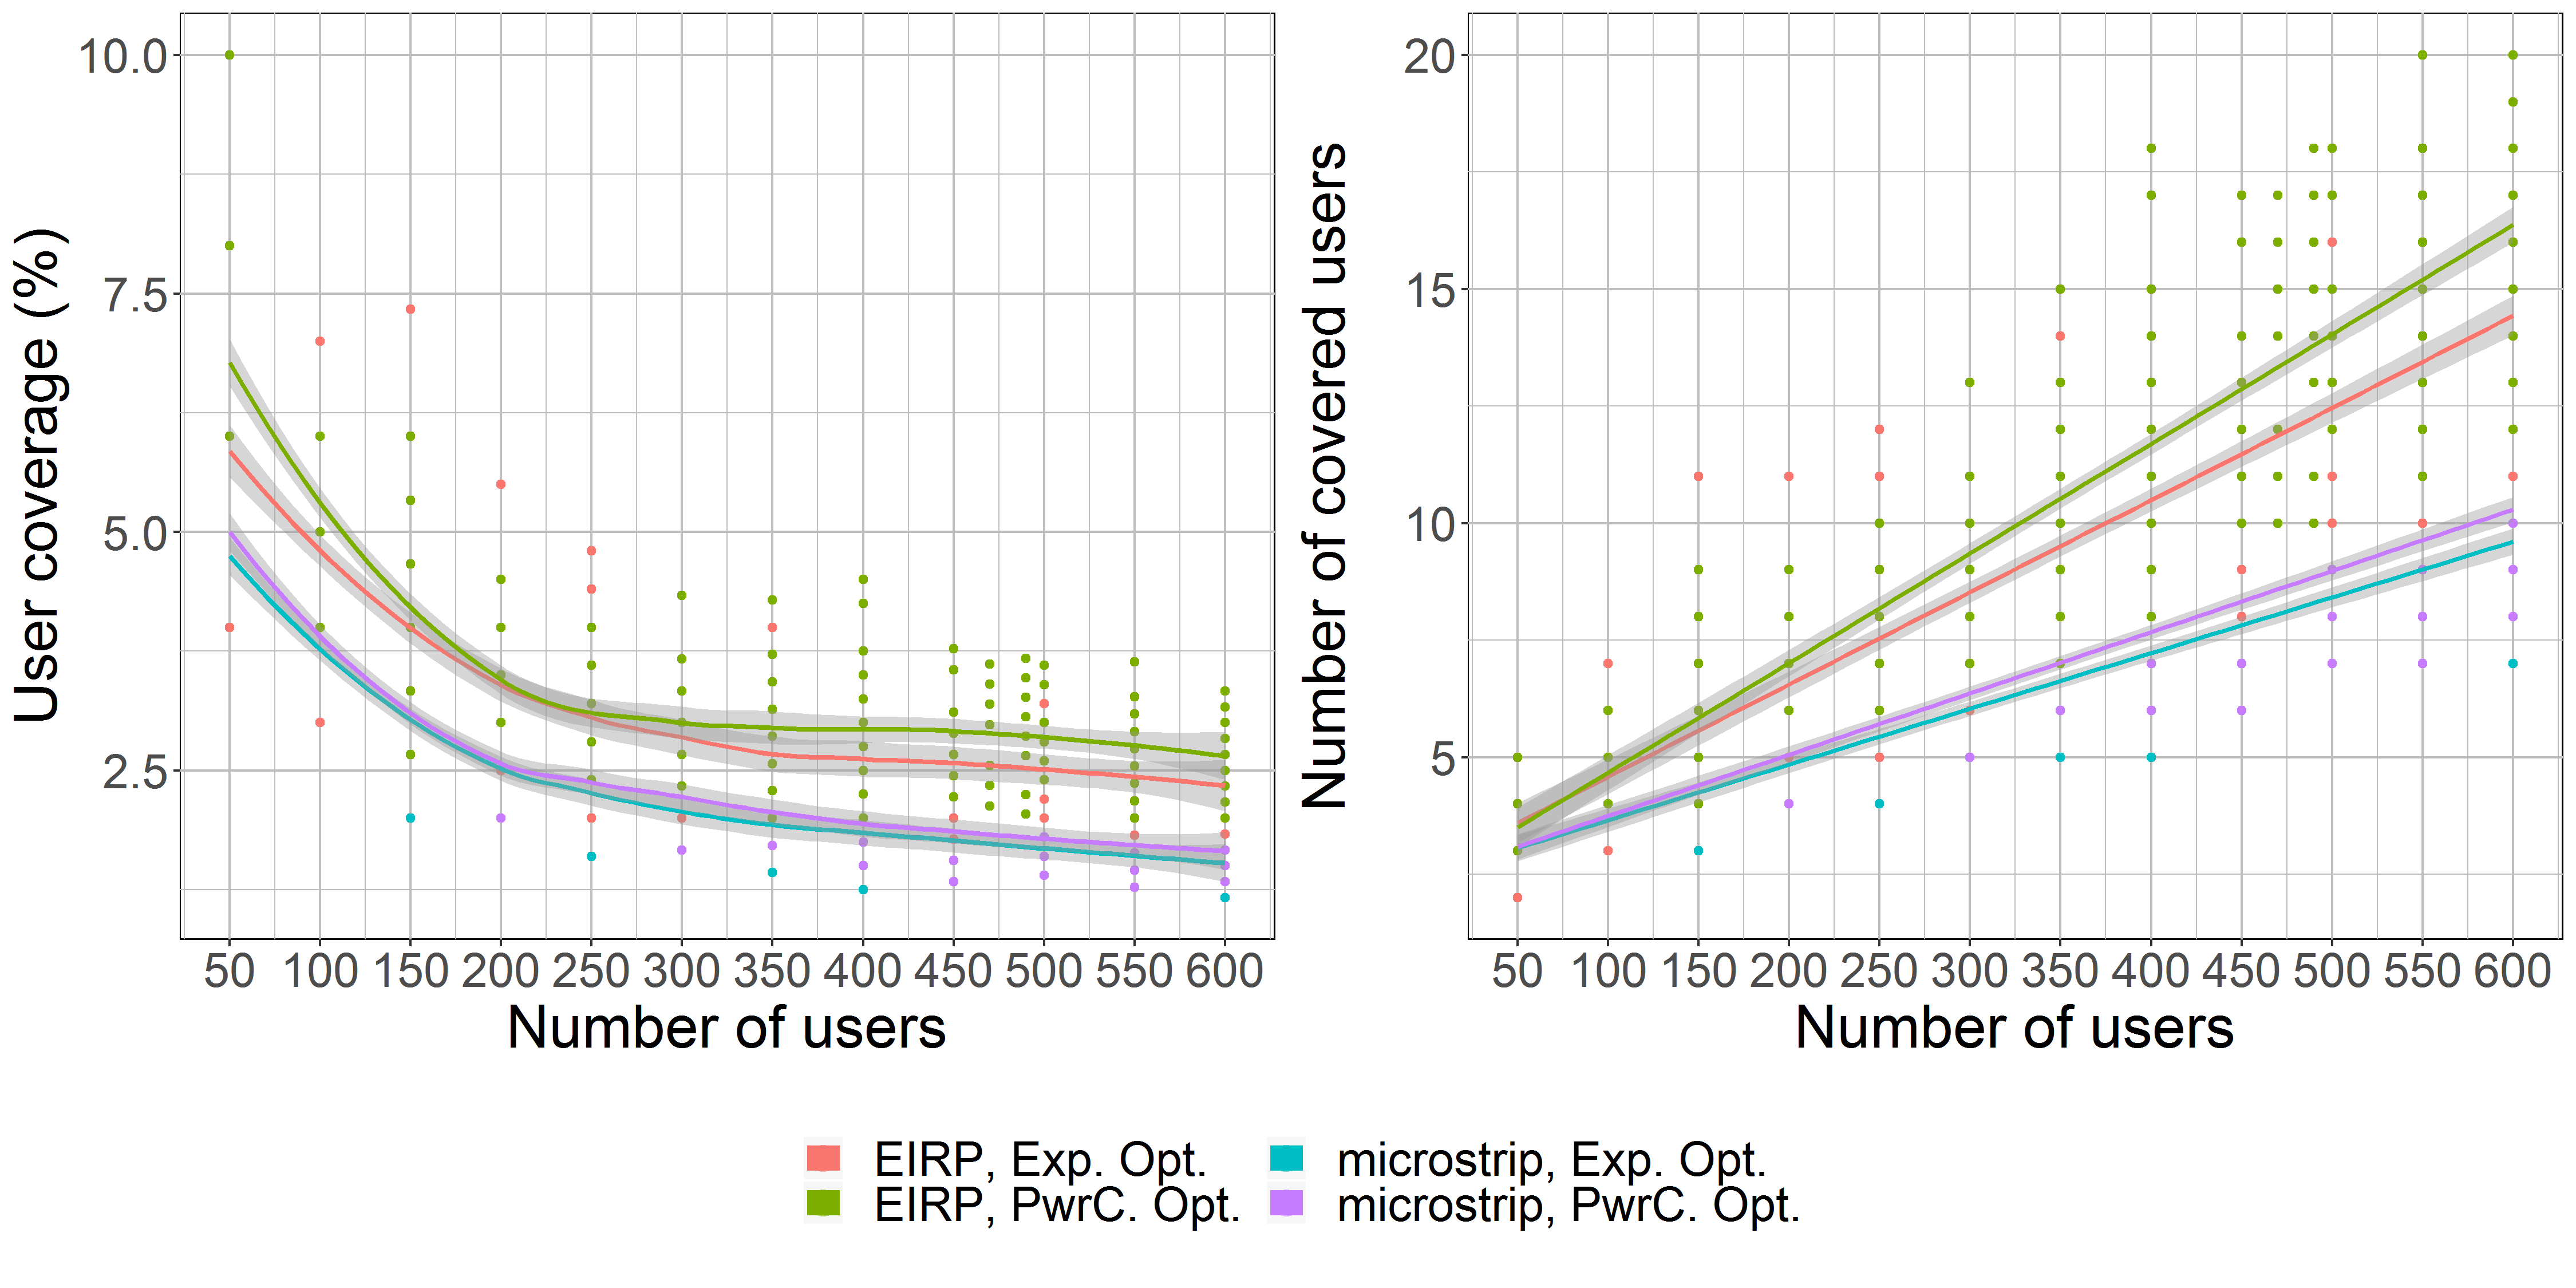
\includegraphics[width=\linewidth]{s2/uvsnumdronesAndCov.png}
  \caption{The influence of increasing traffic on the user coverage.}
  \label{fig:s2uvsnumcovusers}
\end{figure}

For example, with 600 users, 5 to 7 additional 
people can be covered when replacing a microstrip patch antenna with an \gls{isotropicradiator}
and changing an exposure optimized network with an power consumption optimized network will 
cover one or two additional users.


\FloatBarrier
Figure  \ref{fig:s2b_dlAndPc}.a  is influenced by  \ref{fig:s2uvsnumcovusers}.a. When less users are 
covered, the exposure of the average user will decrease as well.
For example, in an EIRP \gls{PwrC Opt} network, 50 users have a 6.75\% coverage which corresponds with a weighted average exposure of  18 $mV/m$
while 600 users with 2.75\% coverage only have 9 $mV/m$.
Further,  figure \ref{fig:s2b_dlAndPc}.b is directly influence by figure \ref{fig:s2uvsnumcovusers}.b. When the \gls{UABS} has to cover more users,
the probability that some of these users have a worse path loss is higher. The \gls{UABS} solves this problem by increasing the 
power consumption. Increasing the population from 50 to 600 will require between 0.05 and 0.1 $W$ more. 
For this scenario, no clear difference in power consumption exists between the four configurations.
\begin{figure}[h!]
  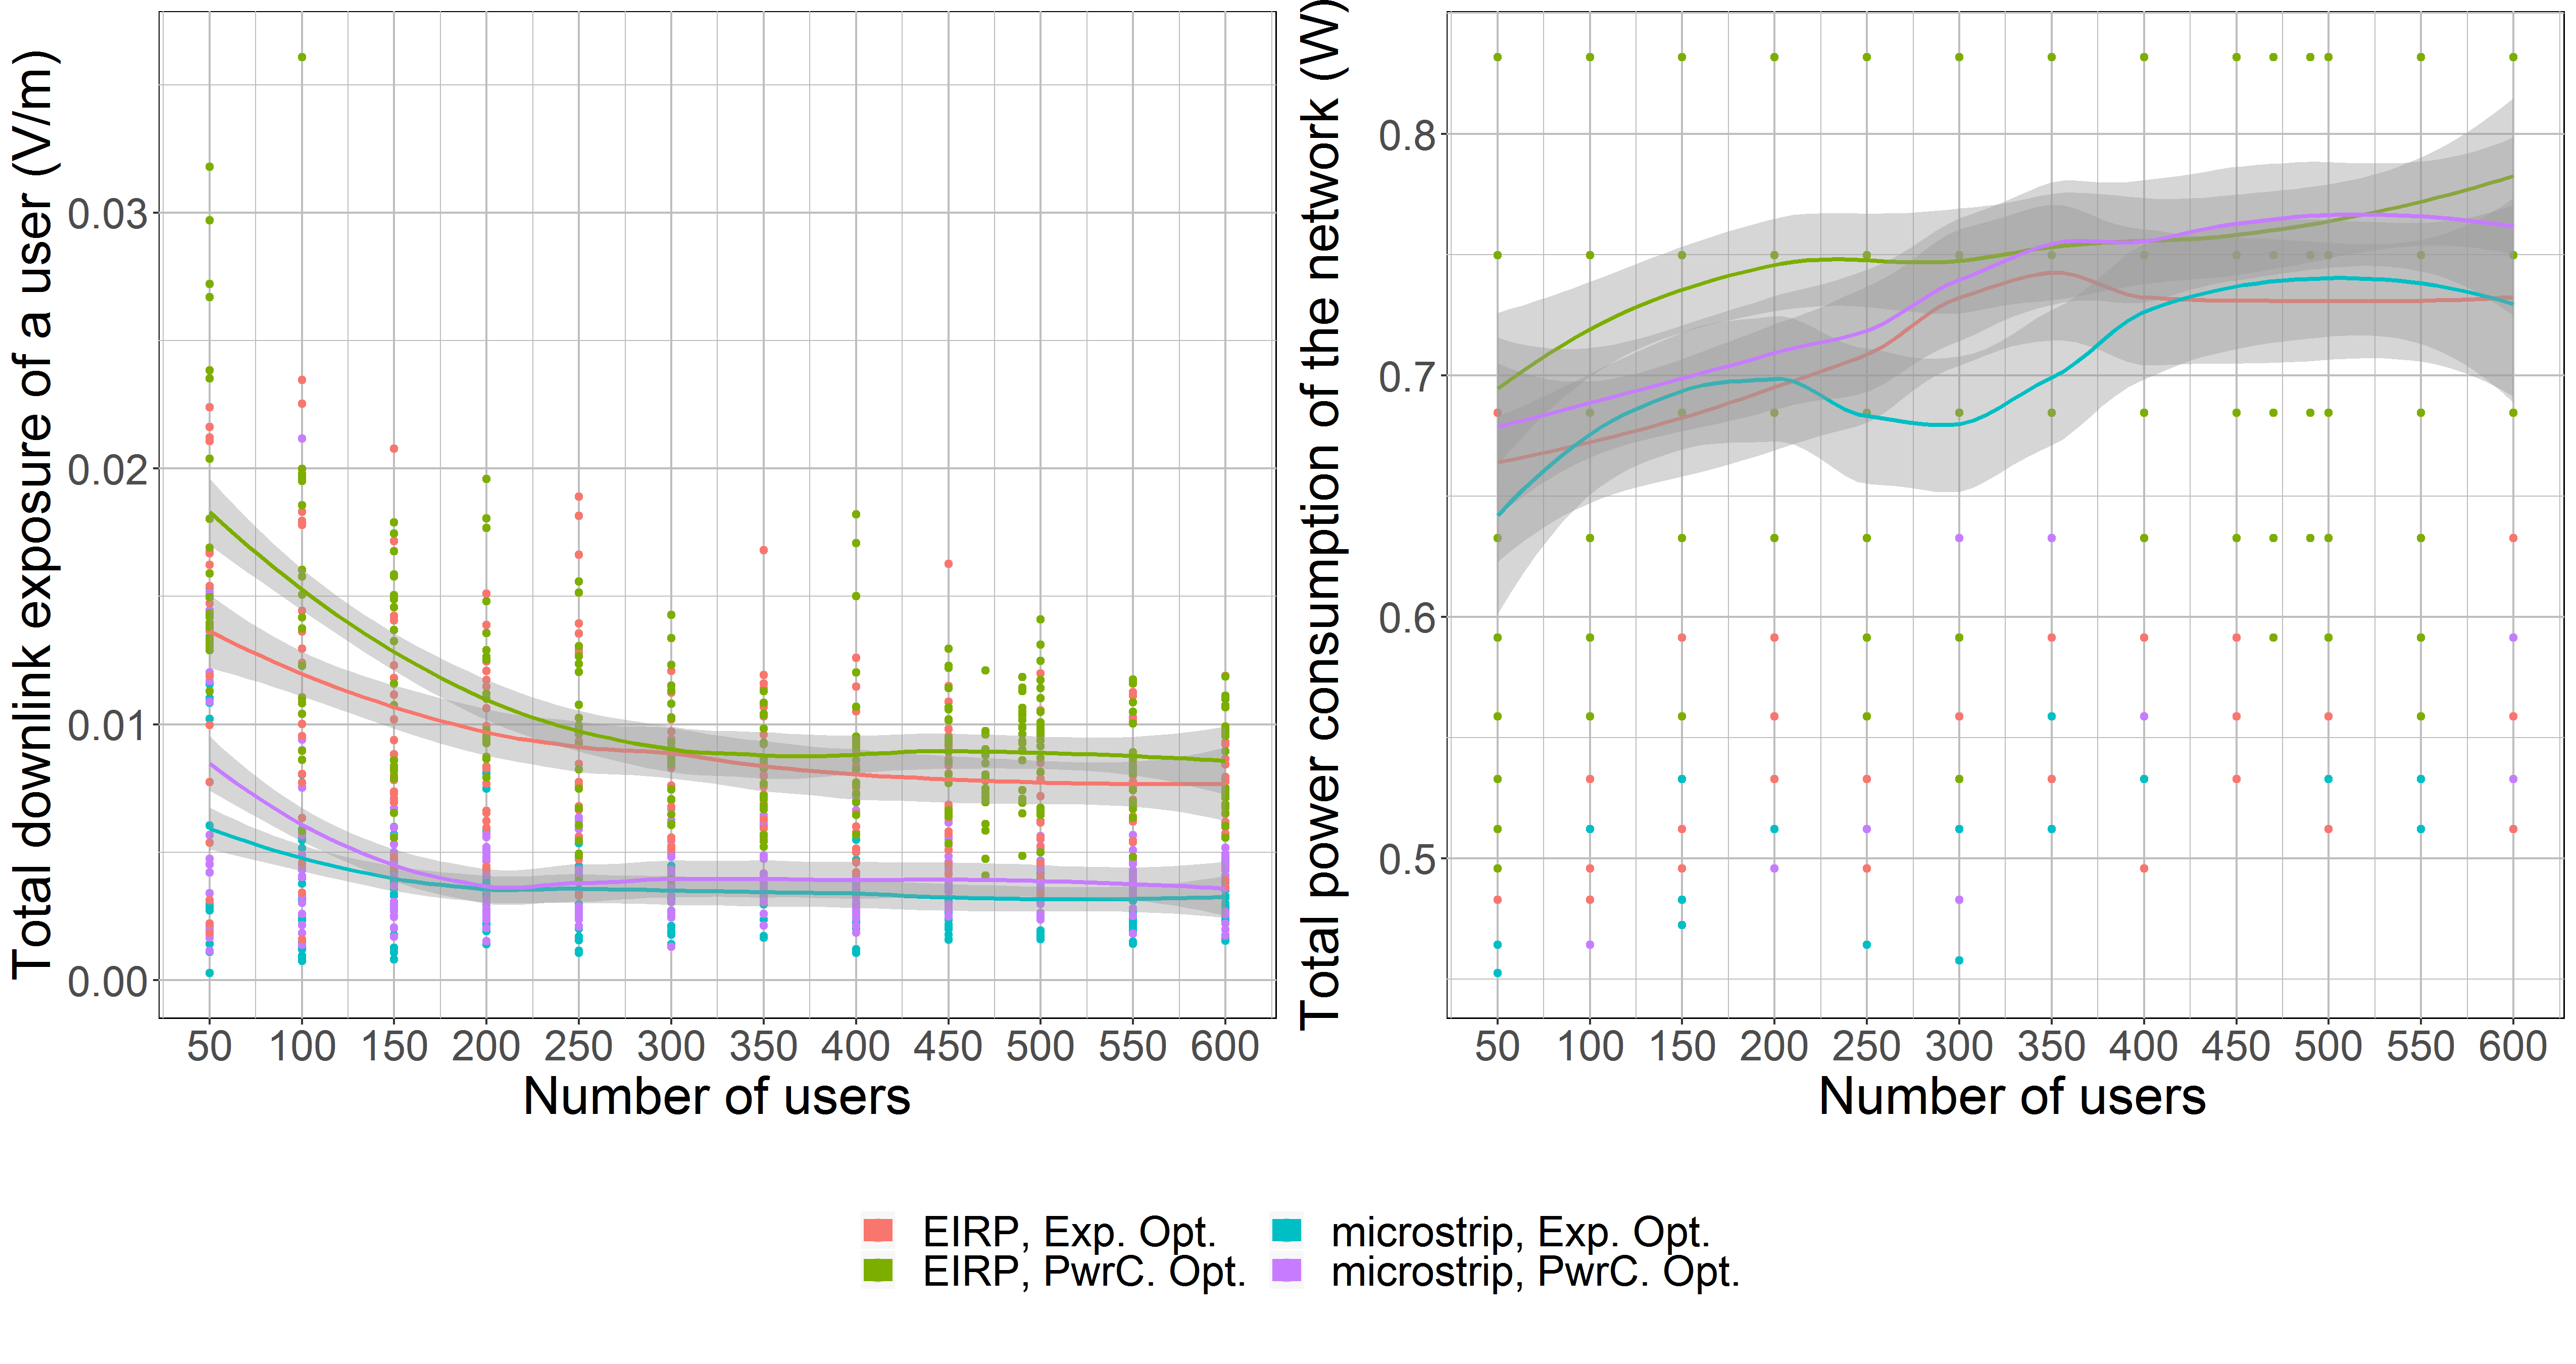
\includegraphics[width=\linewidth]{s2/uvsdlAndPc.png}
  \caption{These two figures show how various sizes of population influence the downlink electromagnetic radiation of the average user (left) and 
  power consumption of the entire network (rights) for one \acs{UABS} available in the network.}
  \label{fig:s2b_dlAndPc}
\end{figure}

The \gls{SAR} coming from the 
users own device is on average zero since most users are uncovered. 
Figure \ref{fig:uvsulsarcentralUsers} shows the exposure for the covered user
just below the \gls{UABS}. Scenario I already showed that the \gls{SAR} from the user's own device is only influenced by the flying height
and is also confirmed by the results in fig. \ref{fig:uvsulsarcentralUsers}.a where constant $SAR^{myUE}$ is measured of 0.15 $\mu W/kg$.
The \gls{SAR} from the \gls{UABS} experiences a slight increase of 0.005 $\mu W/kg$. When the population grows, more users
will be near the \gls{UABS}. The \gls{UABS} will likely decide to cover these users as well as visible in figure \ref{fig:connectionMap}.
\begin{figure}[h]
\subfloat[50 users]{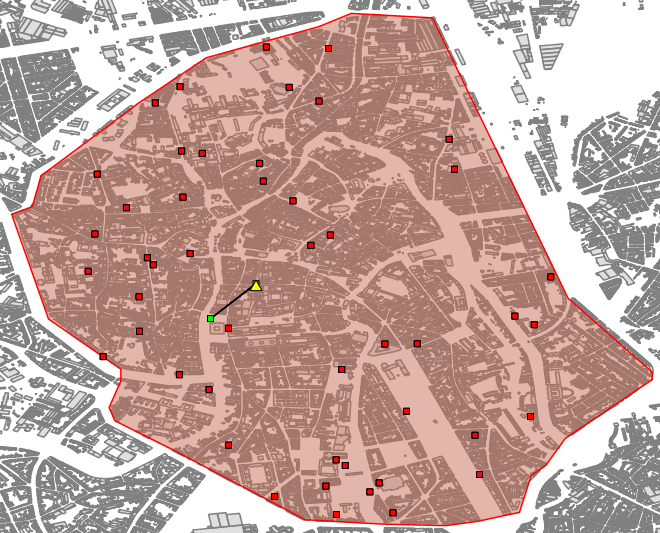
\includegraphics[width=0.49\linewidth]{connectionsMap50Users.png}}
\hfill
\subfloat[600 users]{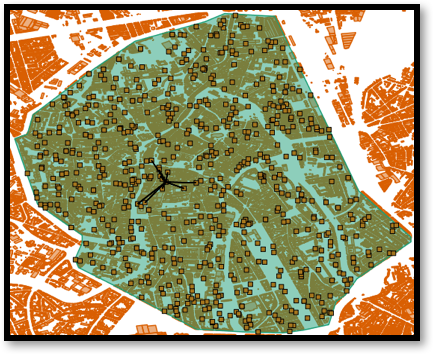
\includegraphics[width=0.49\linewidth]{connectionsMap600Users.png}}
\caption{Overview of which users are connected to the \acs{UABS}.}
  \label{fig:connectionMap}
\end{figure}
\FloatBarrier
These users might have a slightly 
worse path loss because of obstructing buildings or somewhat bigger distance. The \gls{UABS} reacts to this by increasing 
his power consumption causing an increase in the \gls{DL} \gls{SAR} for the central user.
The far-field radiation from \gls{UE} is very low as mentioned before and therefore added separately in figure \ref{fig:uvsulsarcentralUsers}.b.
It shows that the \gls{SAR}  from other \gls{UE} increases from zero to $0.15\ pW/kg$. 
\begin{figure}[h]
\centering
  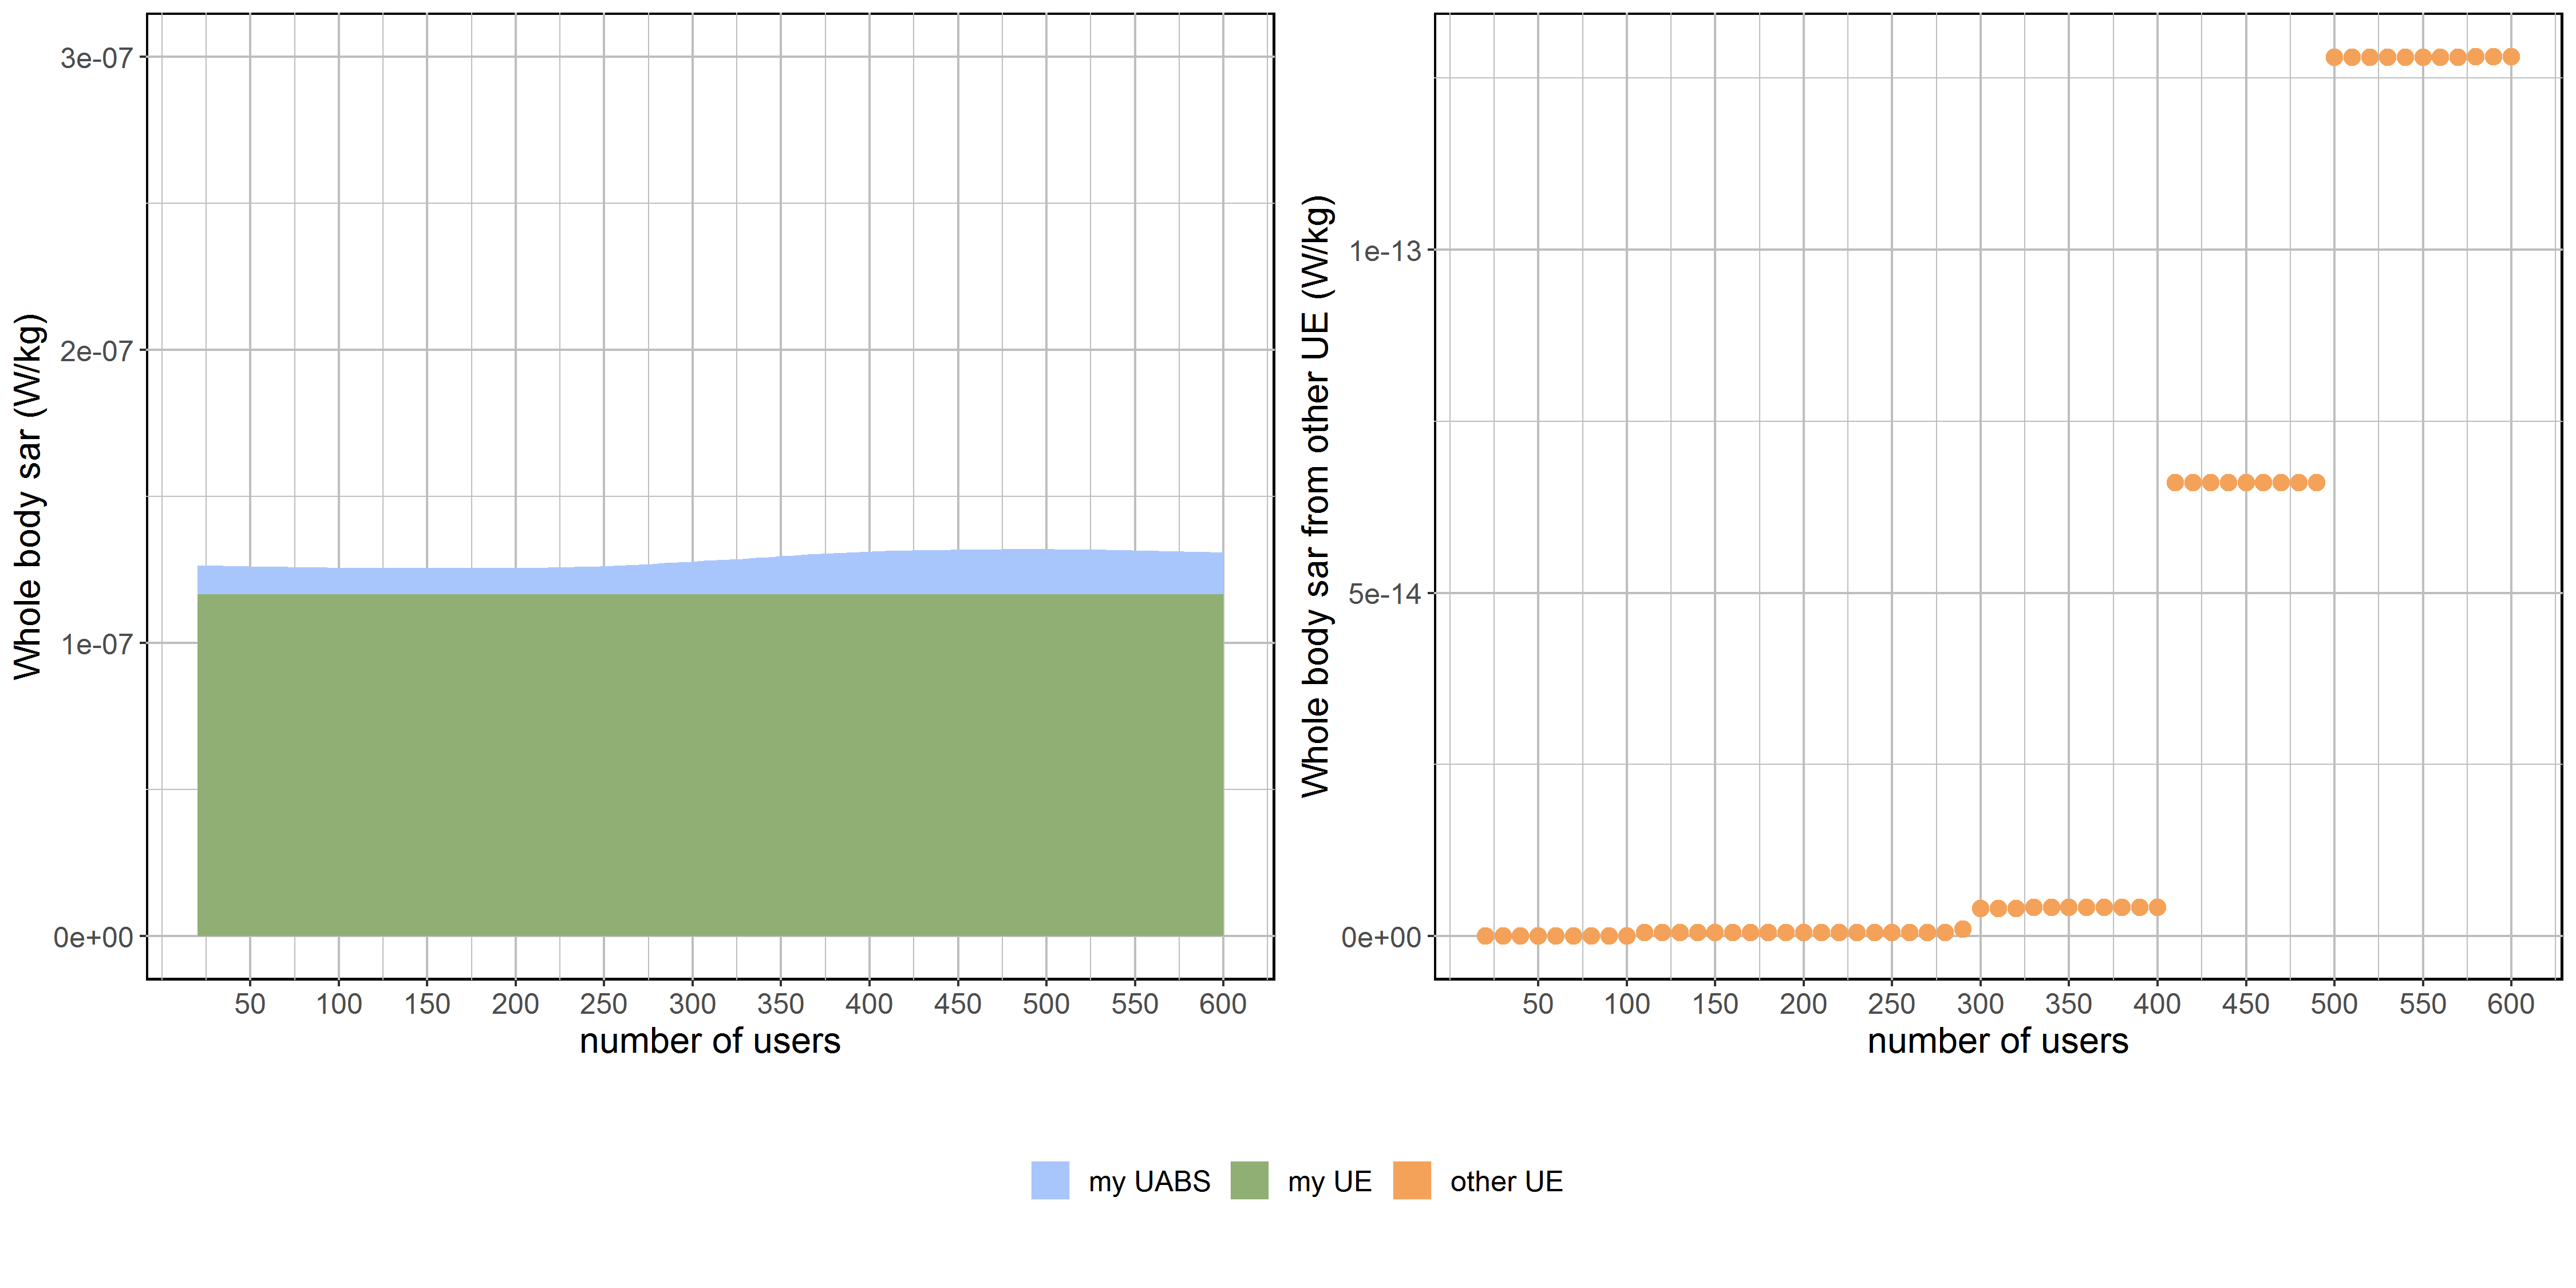
\includegraphics[width=\linewidth]{s2/uvsulsarcentralUser.png}
  \caption{SAR-values for the user who is directly beneath the only \acs{UABS} available.}
  \label{fig:uvsulsarcentralUsers}
\end{figure}

\FloatBarrier
\subsection{Unlimited Number of UABSs}
\subsubsection{Variable Flying Height}
The same scenario as in the previous section is investigated. Only now, an unlimited number of \gls{UABS}s is available.
The results prove that the different optimization strategies work as intended.
A \gls{PwrC Opt} network has indeed a lower power consumption but therefore result in higher electromagnetic radiation.
On the other hand, an \gls{Exp Opt} network will reduce the electromagnetic exposure by using more \gls{UAV}s and thence also increase the network's
power consumption. This conclusion was already made in \cite{J1} and is supported by these results.
For example, when comparing both optimization strategies for the same \gls{isotropicradiator} and the same default flying height, we see that
the power consumption optimized network requires 51 $W$ and therefore exposes its users
to $15\ mV/m$. When optimizing towards electromagnetic radiation, the exposure drops to $11.5\ mV/m$ but at a cost of a higher power consumption
of $54\ W$.
\begin{figure}[h!]
  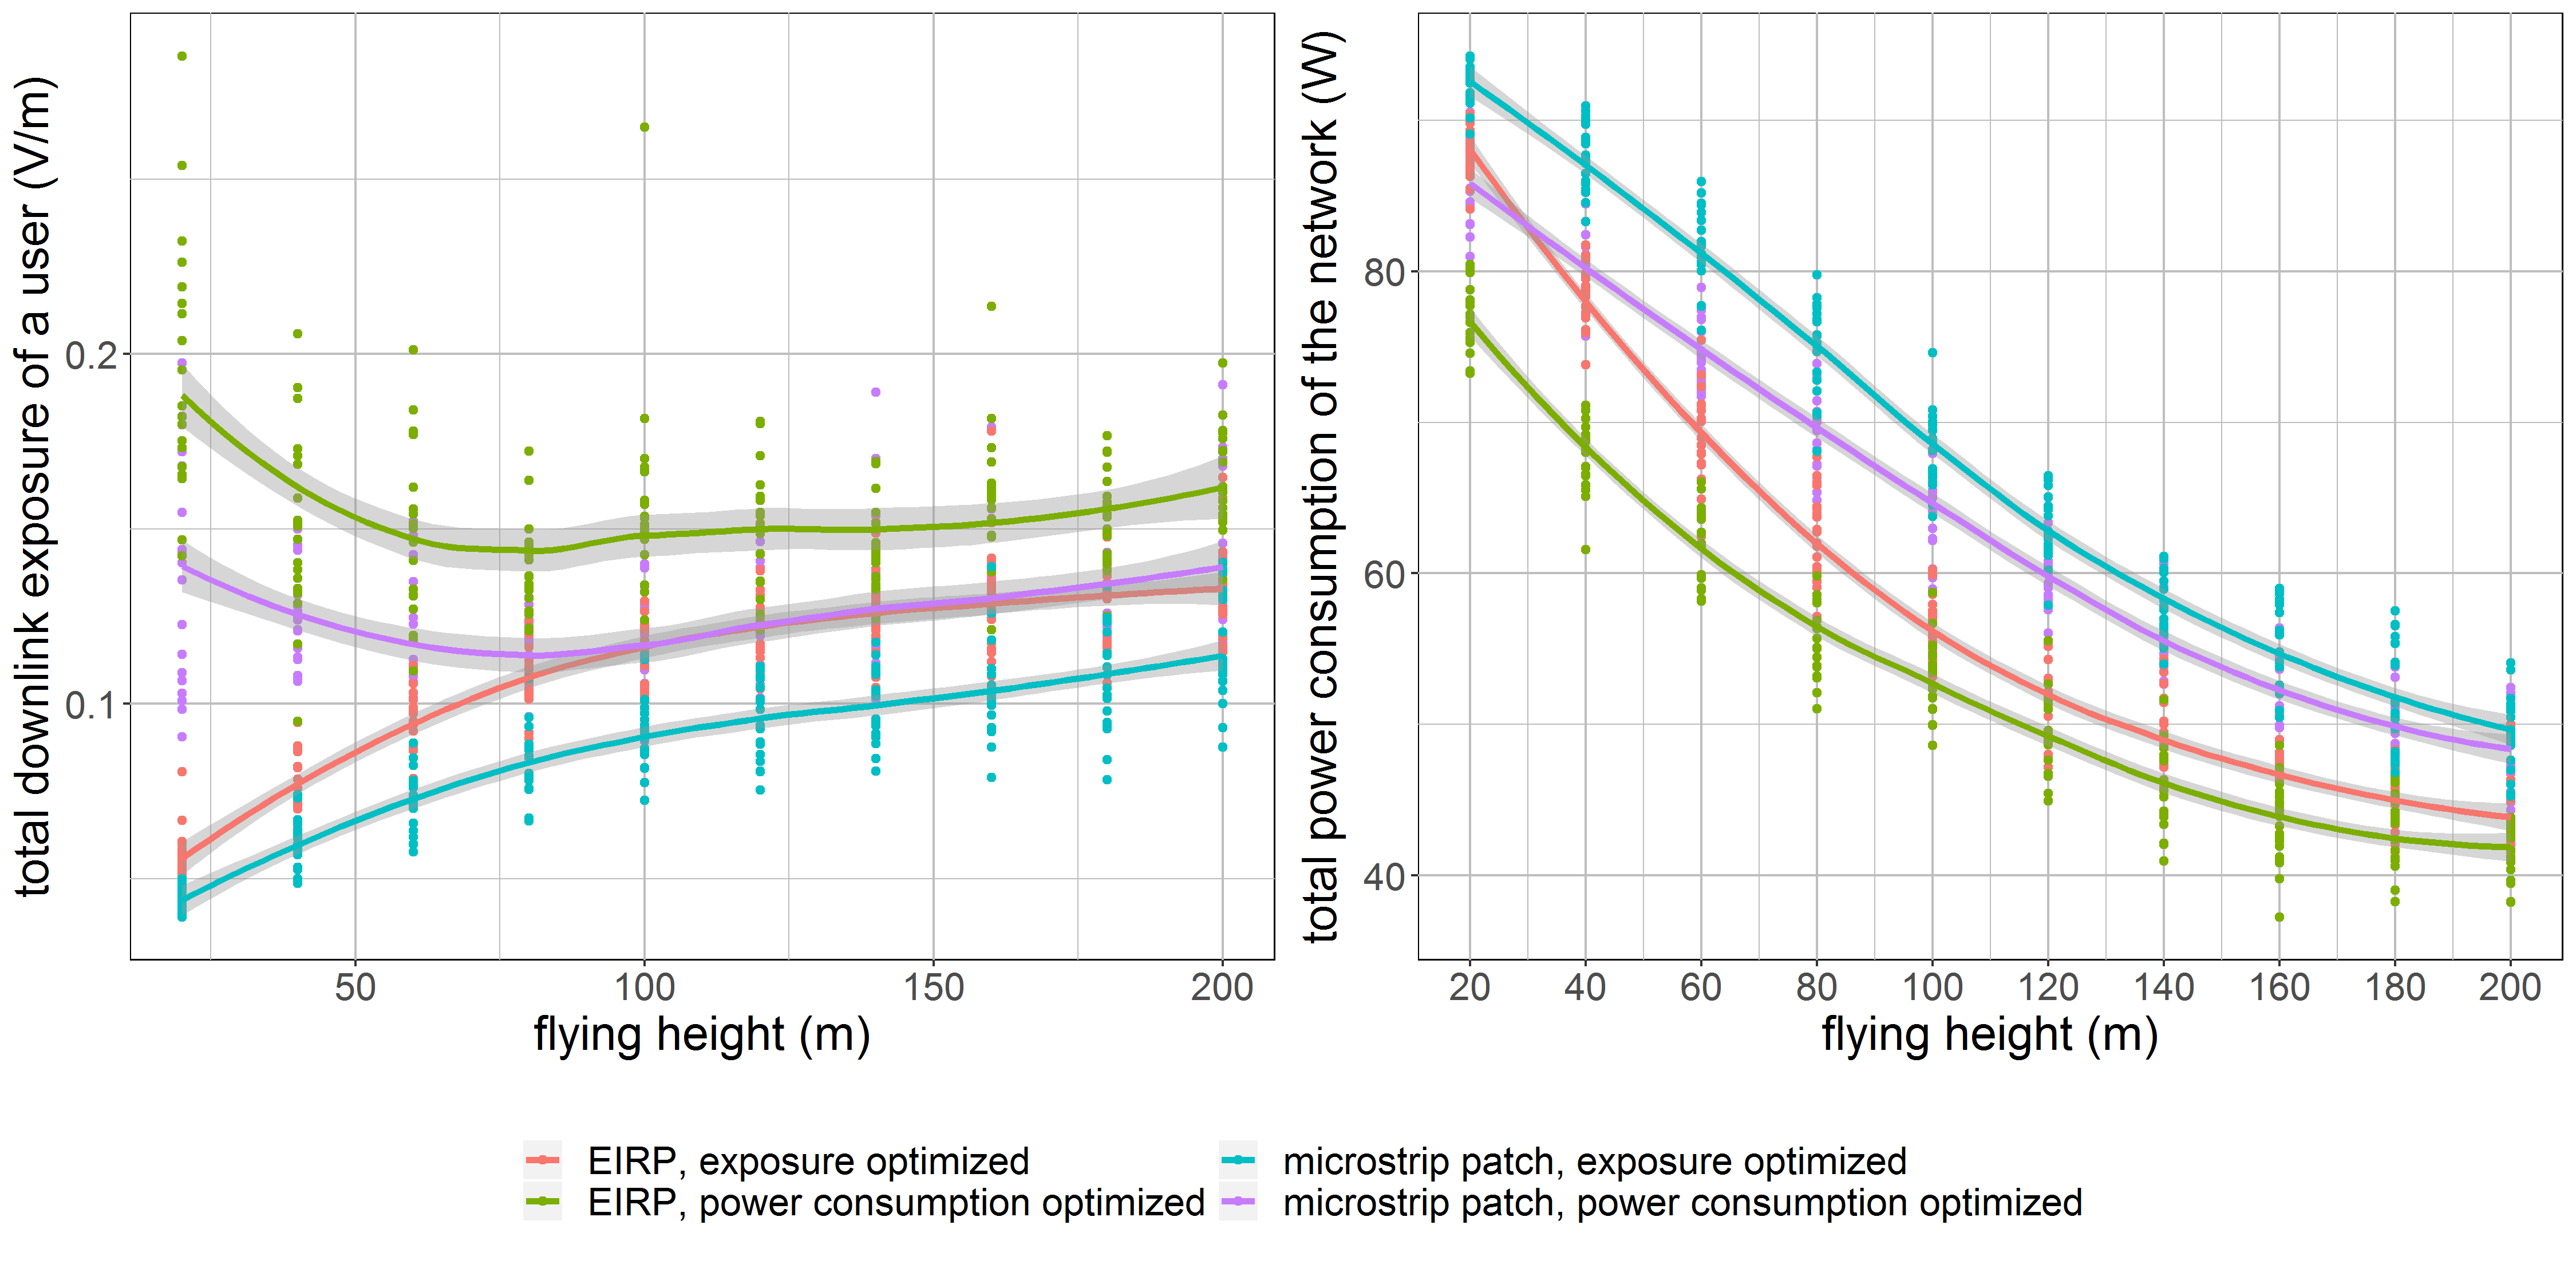
\includegraphics[width=\linewidth]{../results/s3/fhvsdlAndPc.png}
  \caption{These two figures show how the flying height influences the downlink electromagnetic radiation of the average user (left) and 
  power consumption of the entire network (right) for an unlimited number of \gls{UAV}s.}
  \label{fig:s3a_dlAndPc}
\end{figure}

The exposure in figure \ref{fig:s3a_dlAndPc} shows that an \gls{Exp Opt} network increases logarithmically while the \gls{PwrC Opt} network rather 
has a concave relationship with the flying height, and has its lowest point at around 70 metres.

Figure \ref{fig:s3a_numdronesAndCov}.a shows that the optimal coverage is achieved at a low flying height of 
40 metres with around 99\% coverage. 
However, there is a downside to this. 
Figure \ref{fig:s3a_numdronesAndCov}.b 
 shows that the number of required \gls{UAV}s increases when the flying altitude becomes lower;
a behaviour which was also determined in \cite{J2}.
For example, an microstrip \gls{Exp Opt} network and an \gls{EIRP} \gls{PwrC Opt} network require respectively 84 and 64
\gls{UABS}s at a flying altitude of $200\ m$ which increases respectively to 211 and 162 \gls{UABS}s at a much lower flying altitude of $20\ m$.

\begin{figure}[]
  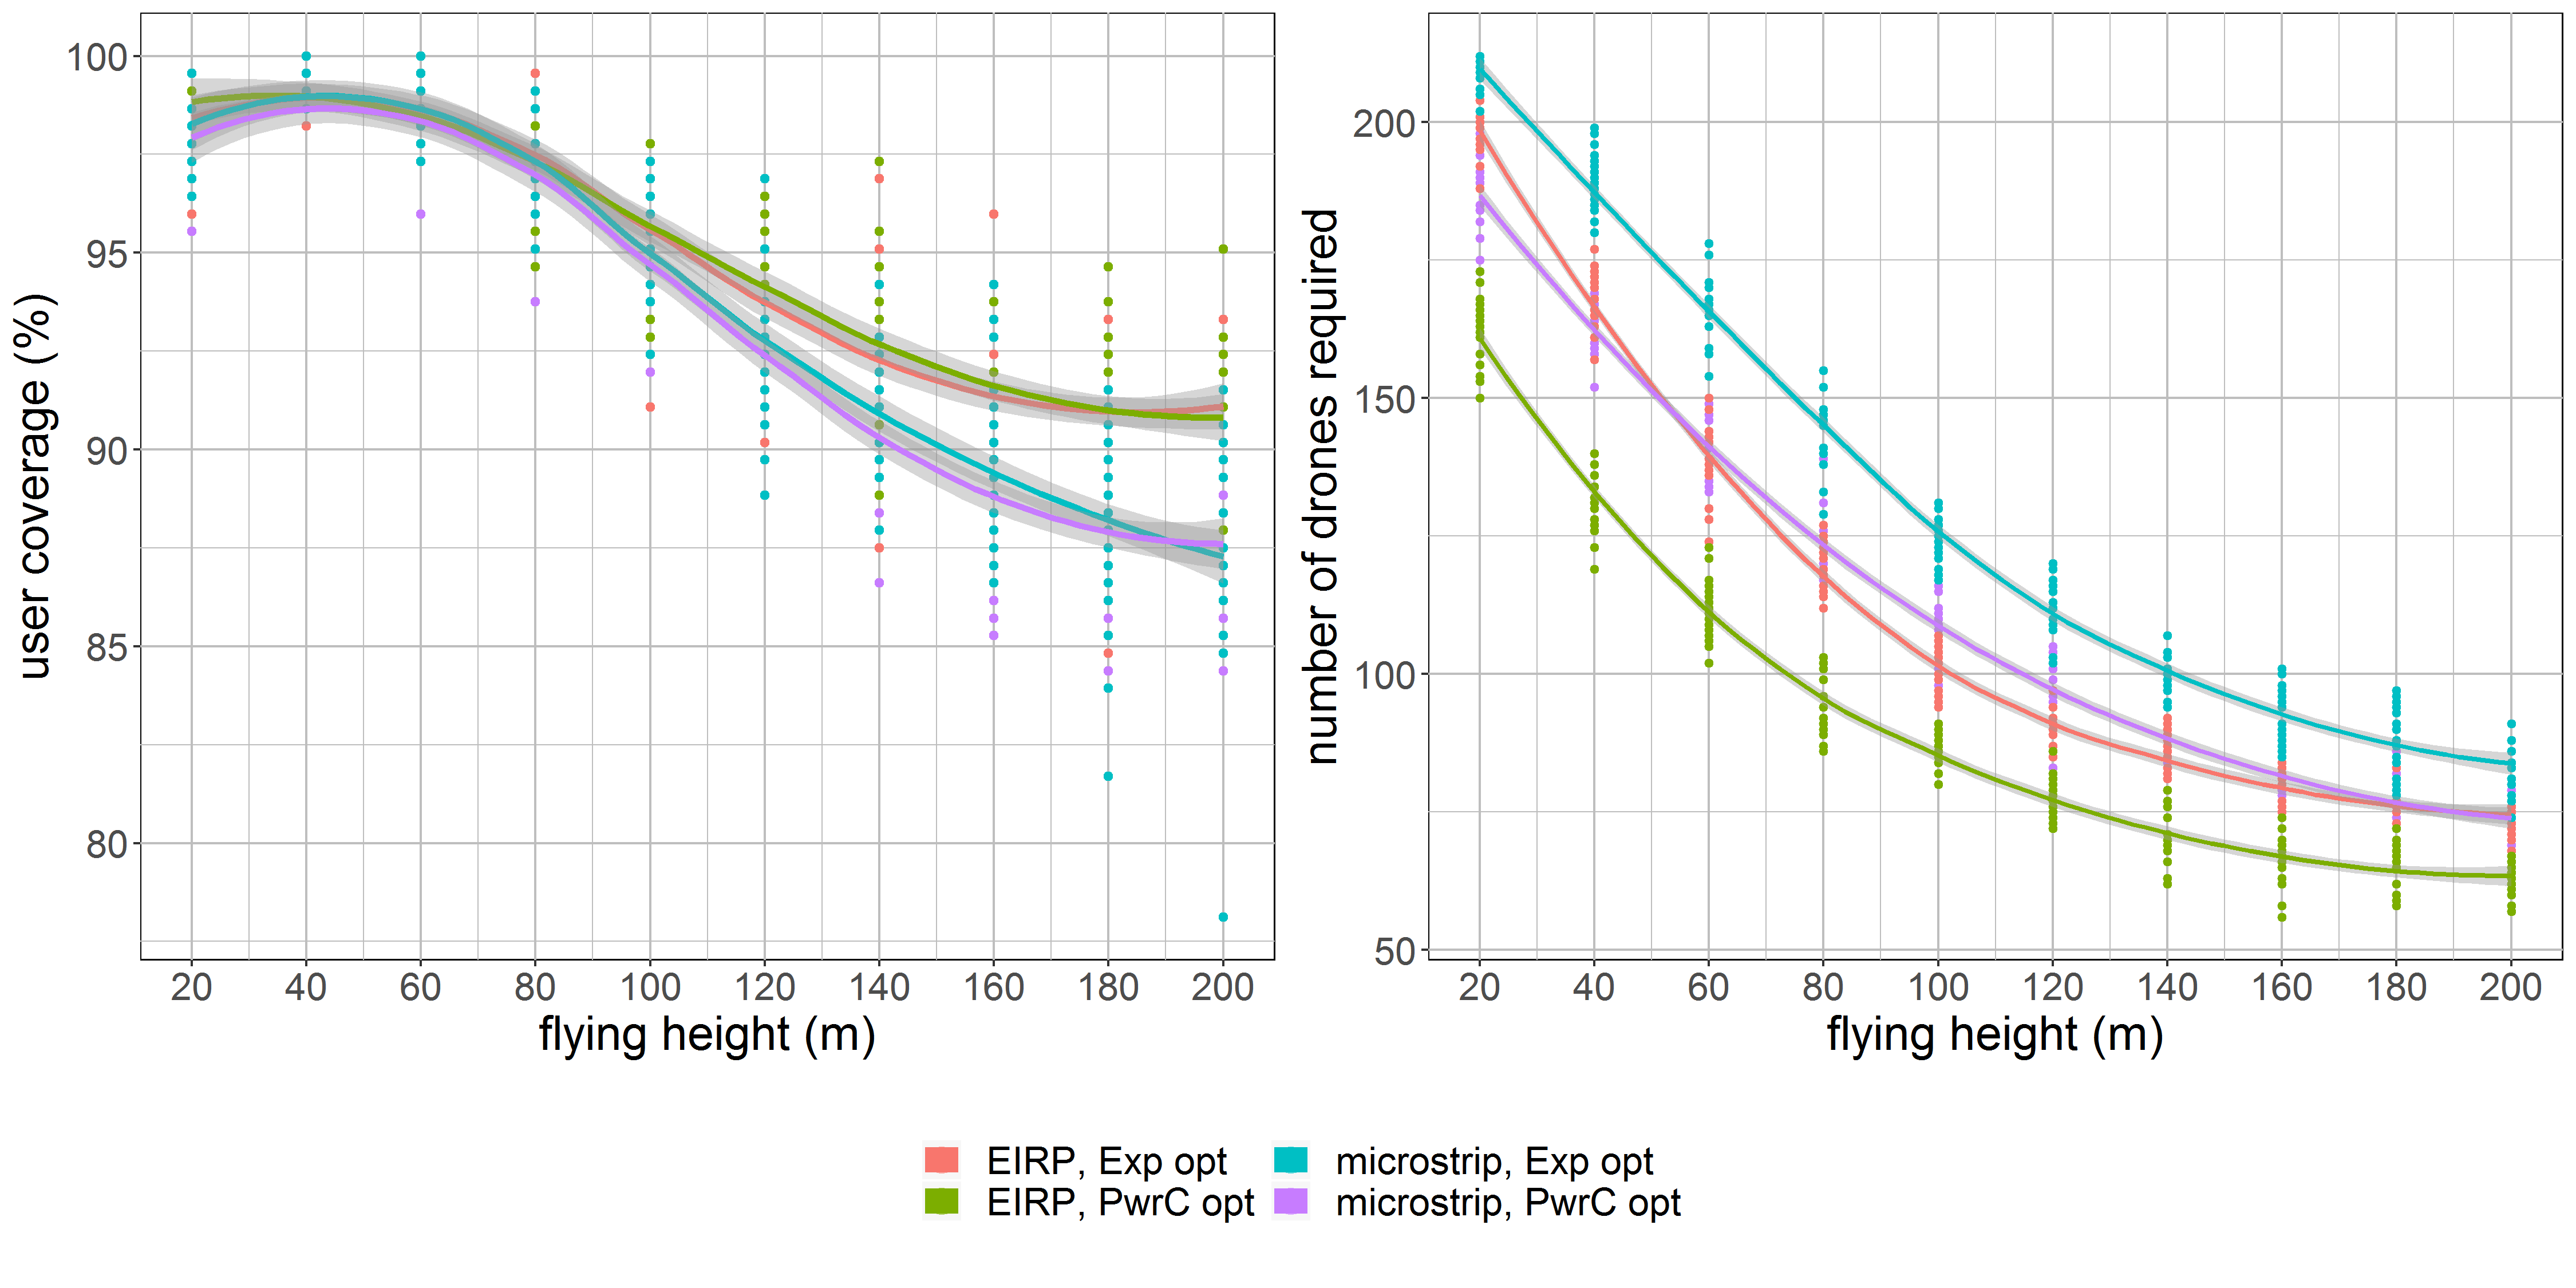
\includegraphics[width=\linewidth]{../results/s3/fhvsnumdronesAndCov.png}
  \caption{This graph shows how much \acs{UAV}s are required at different flying heights while trying to achieve a 100\% coverage.}
  \label{fig:s3a_numdronesAndCov}
\end{figure}

Figure \ref{fig:s3a_fourSourcesMatrix} shows how each source contributes to the total \gls{SAR}.
A first consequence of raising the flying altitude from 
 20 to 200 metres is the increase \gls{SAR} from the user's own device situated
 with 89 and 141 $nW/kg$; a behaviour also explained in the first scenario.
Figure \ref{fig:s3a_fourSourcesMatrix} shows that once the flying altitude surpasses the \gls{NLOS} of the buildings, 
around 70 to 80 metres, the SAR from the serving \gls{UABS} remains 
more or less constant for all configurations.
The $SAR^{myUABS}$ varies for these higher flying heights 
around $160\ nW/kg$ for microstrip \gls{PwrC Opt} networks and around $98\ nW/kg$ for microstrip \gls{Exp Opt} and \gls{EIRP} \gls{PwrC Opt} networks.
An \gls{EIRP} \gls{Exp Opt} network is situated around $47\ nW/kg$.
These higher flying altitudes will also result in an increase in electromagnetic radiation from 
other \gls{UABS}s.
Raising the flying altitude from 20 to 200 metres will increase the
the $SAR^{otherUABS}$ between 115 and 140 $nW/kg$ for \gls{EIRP} antennae and between 54 and 74 $nW/kg$ for microstrip patch antennae
for both optimization strategies.


\begin{figure}[h!]
  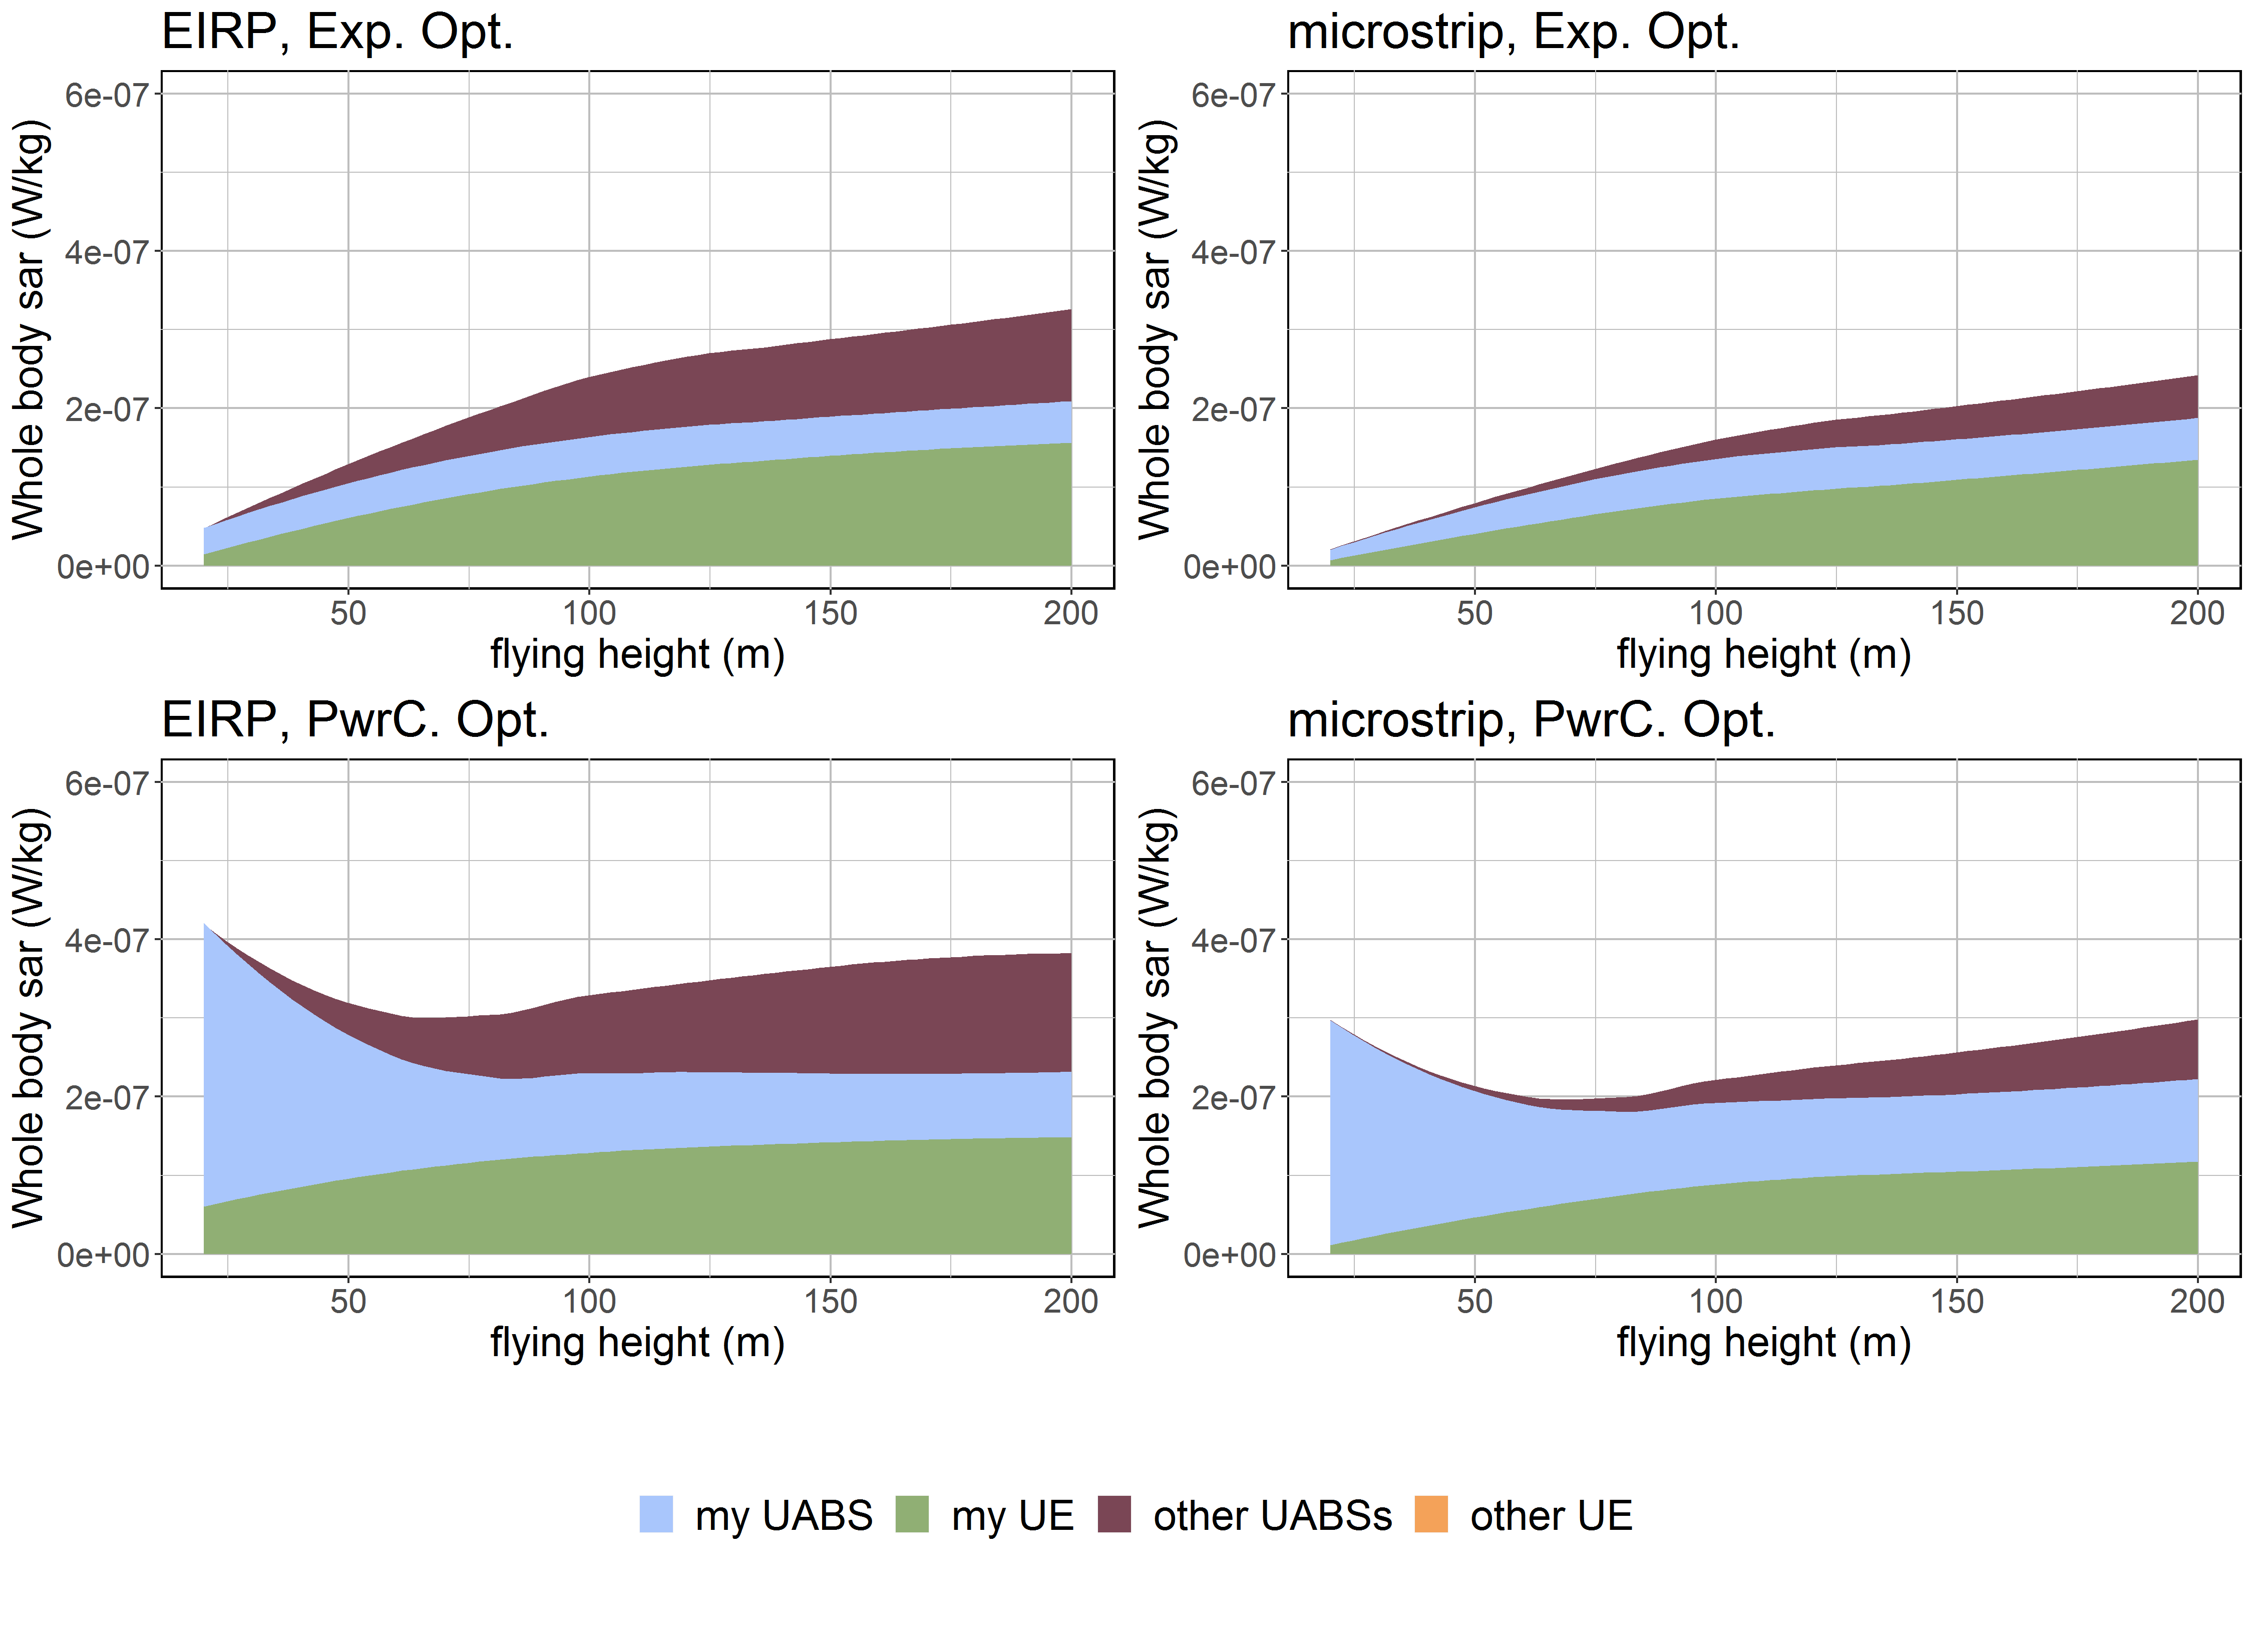
\includegraphics[width=\linewidth]{../results/s3/fhFourSources.png}
  \caption{Each chart corresponds with one of the four possible configurations. The contribution of each source towards the total 
  \acs{SAR} for a varying flying height is shown.}
  \label{fig:s3a_fourSourcesMatrix}
\end{figure}

\FloatBarrier
\subsubsection{Variable Number of Users}

The second evaluated parameter of this scenario is a variable number of users while the flying height is fixed to 100 metres.  
Figure \ref{fig:s3b_numdronesAndCov}.a shows how the tool tries to reach a 100\% coverage. The percentage
of covered users is slightly less for smaller networks. For only 50 users, an average 
coverage of around 93\% is achieved while a network with 600 users has a coverage of around 97\%.
Figure \ref{fig:s3b_numdronesAndCov}.b prove that more \gls{UAV}s are required for these large 
populations. 
The difference in optimization strategy is very little for a small amount of people but increases very quickly. 
When the population increases from 50 to 600 users,
 200 more \gls{UABS}s are required by a microstrip \gls{Exp Opt} network,
 around 130 more \gls{UABS}s for an \gls{EIRP} \gls{Exp Opt} network or a microstrip \gls{PwrC Opt} network
 and 110 more \gls{UABS}s for an \gls{EIRP} \gls{PwrC Opt} network.
This is an expected behaviour  when looking at the previous scenario where, with only one \gls{UABS} available, 
the percentage of covered users decreases for these larger populations.

\begin{figure}[h]
  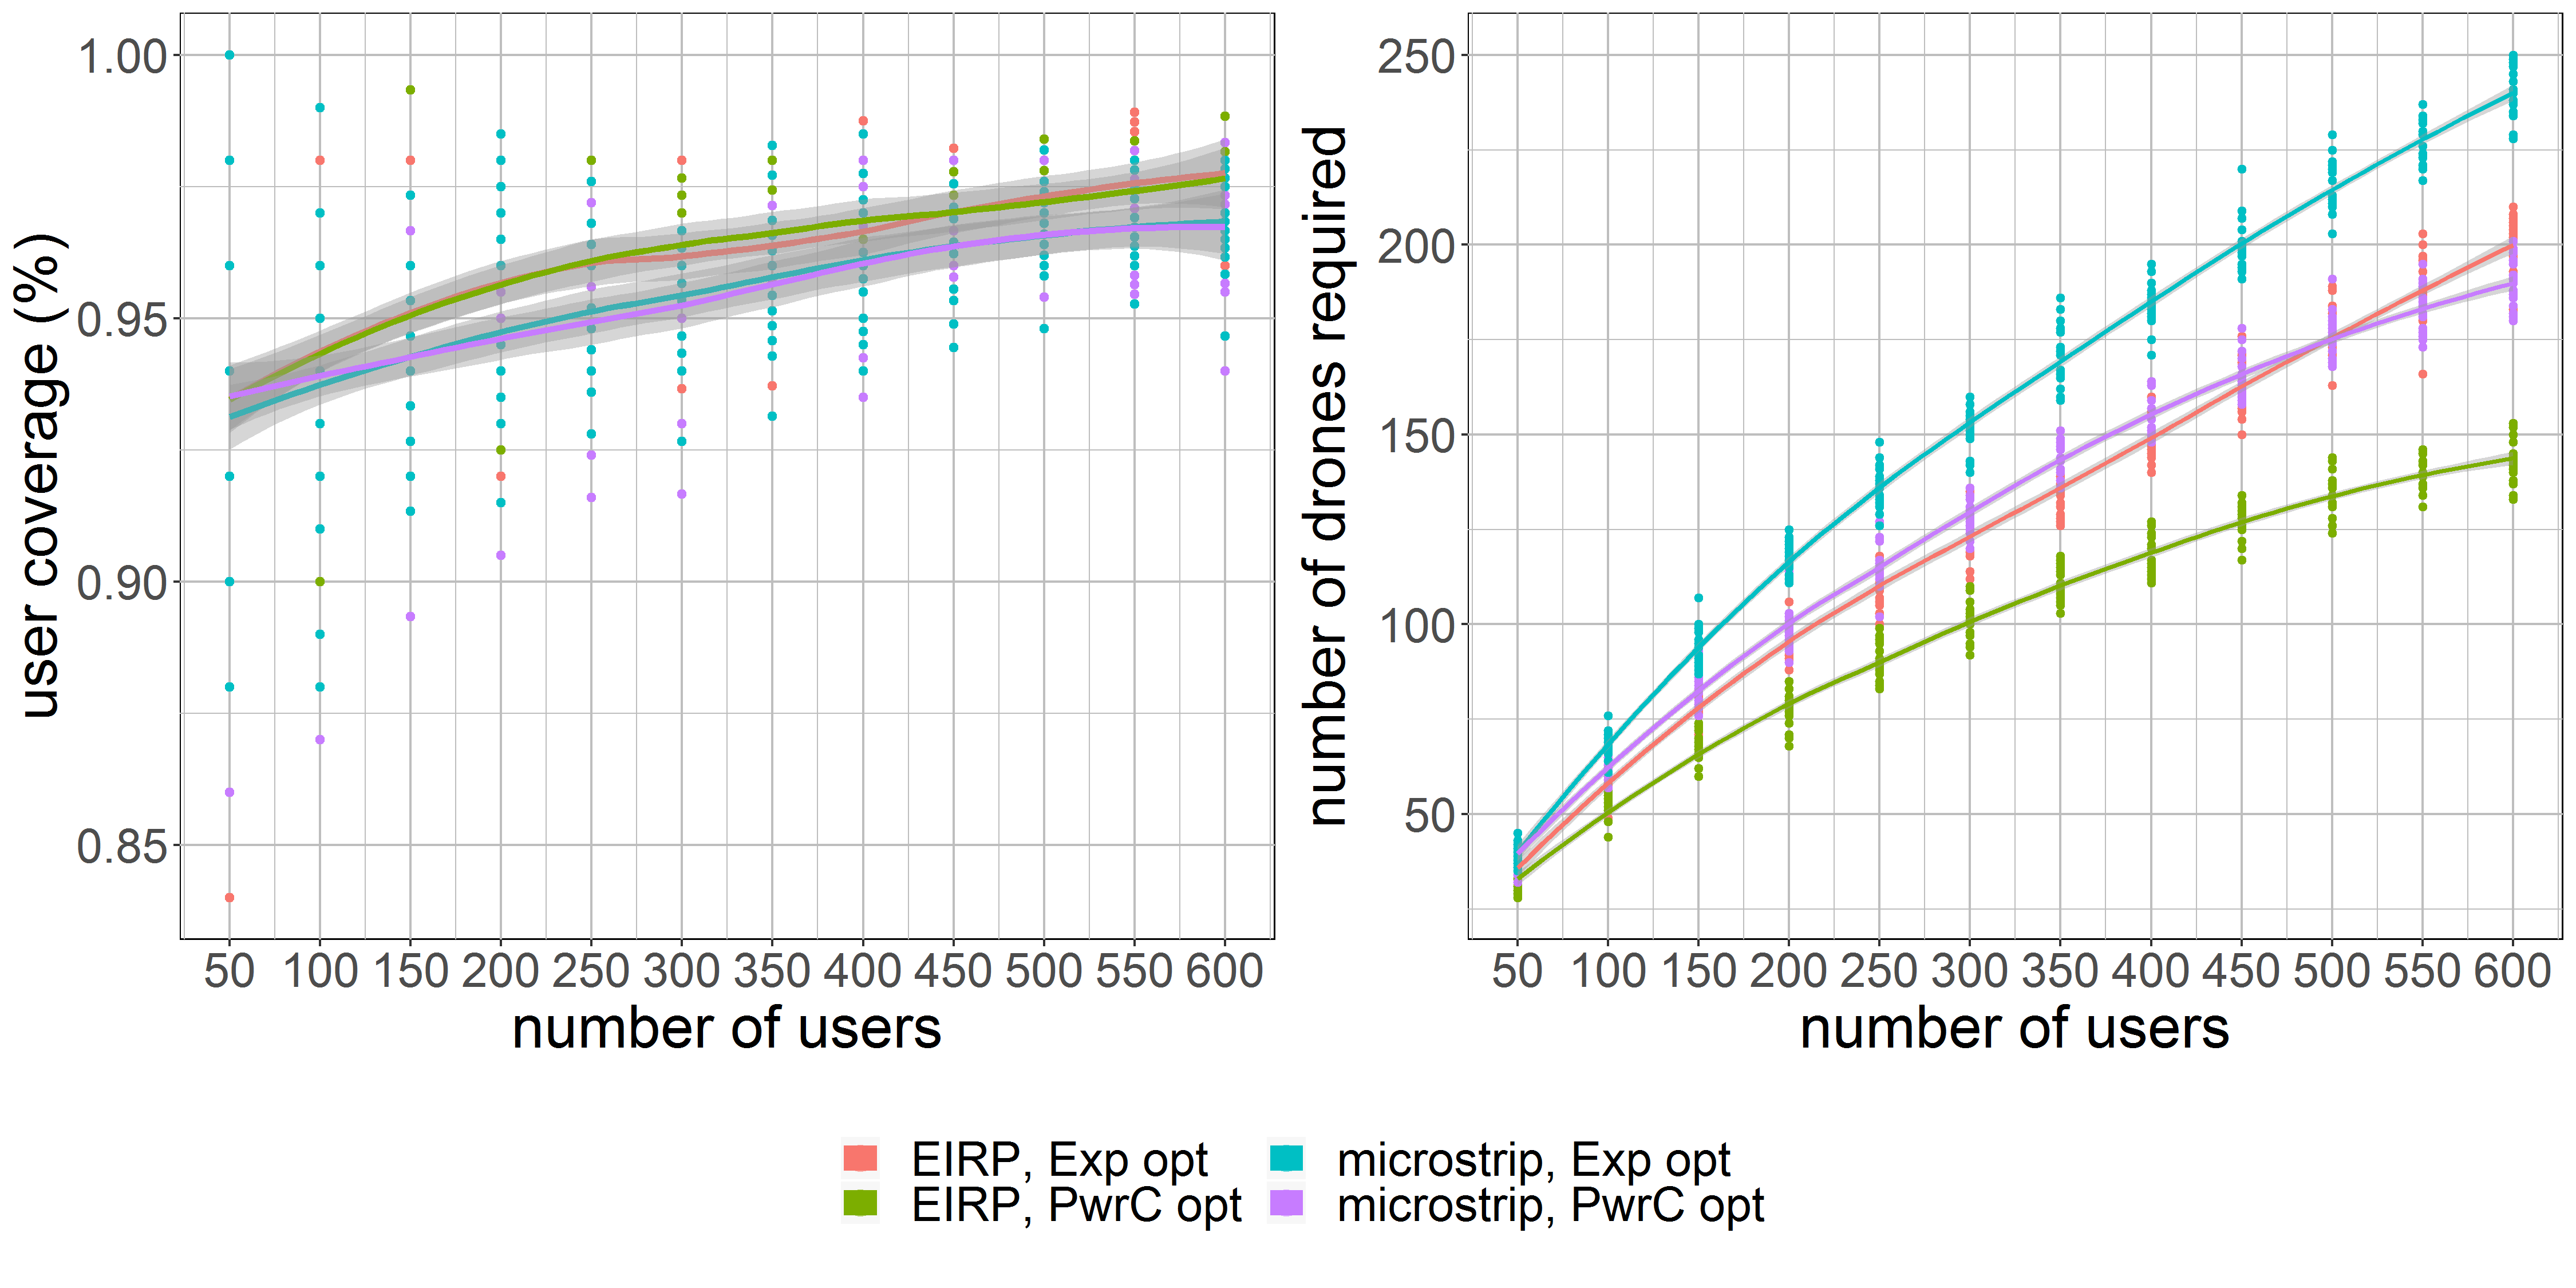
\includegraphics[width=\linewidth]{../results/s3/uvsnumdronesAndCov.png}
  \caption{This graph shows how much \acs{UAV}s are required for different flying heights while trying to achieve a 100\% coverage.}
  \label{fig:s3b_numdronesAndCov}
\end{figure}


Figure \ref{fig:s3b_dlAndPC} shows that the electromagnetic radiation and power consumption increase for larger 
populations which is normal since more \gls{UABS}s will be available.
When the population increases from 50 to 600 users, the electromagnetic radiation increases 
between 80 and 130 $mV/m$ depending on the configuration. The power consumption with 50 users is for all configurations around 
20 $W$. Once the population is increased to 600 users, a microstrip \gls{Exp Opt} network will require 130 $W$, 
 a microstrip \gls{PwrC Opt} network requires 117 $W$,
\gls{EIRP} \gls{Exp Opt} networks require 107 $W$ and \gls{EIRP} \gls{PwrC Opt} network requires 92 $W$.

The correct behaviour of the decision algorithm became already clear in the previous subsection but is also
confirmed here. 
When comparing both optimization strategies, a power consumption optimized network requires around 5 $W$ less but exposes its users between 27 $mV/m$ and 30 $mV/m$ more than
exposure optimized networks. 
Further, it is also noticed that \gls{isotropicradiator}s cause more electromagnetic radiation for less energy
compared to microstrip patch antennae. 
When comparing the two types of antennae for a default number of 224 users, 
an \gls{isotropicradiator} will expose the average user 
between 25 $mV/m$ and 27 $mV/m$ more while requiring around 12 $W$ less than when the network would be using a microstrip patch antennae.


\begin{figure}[h!]
  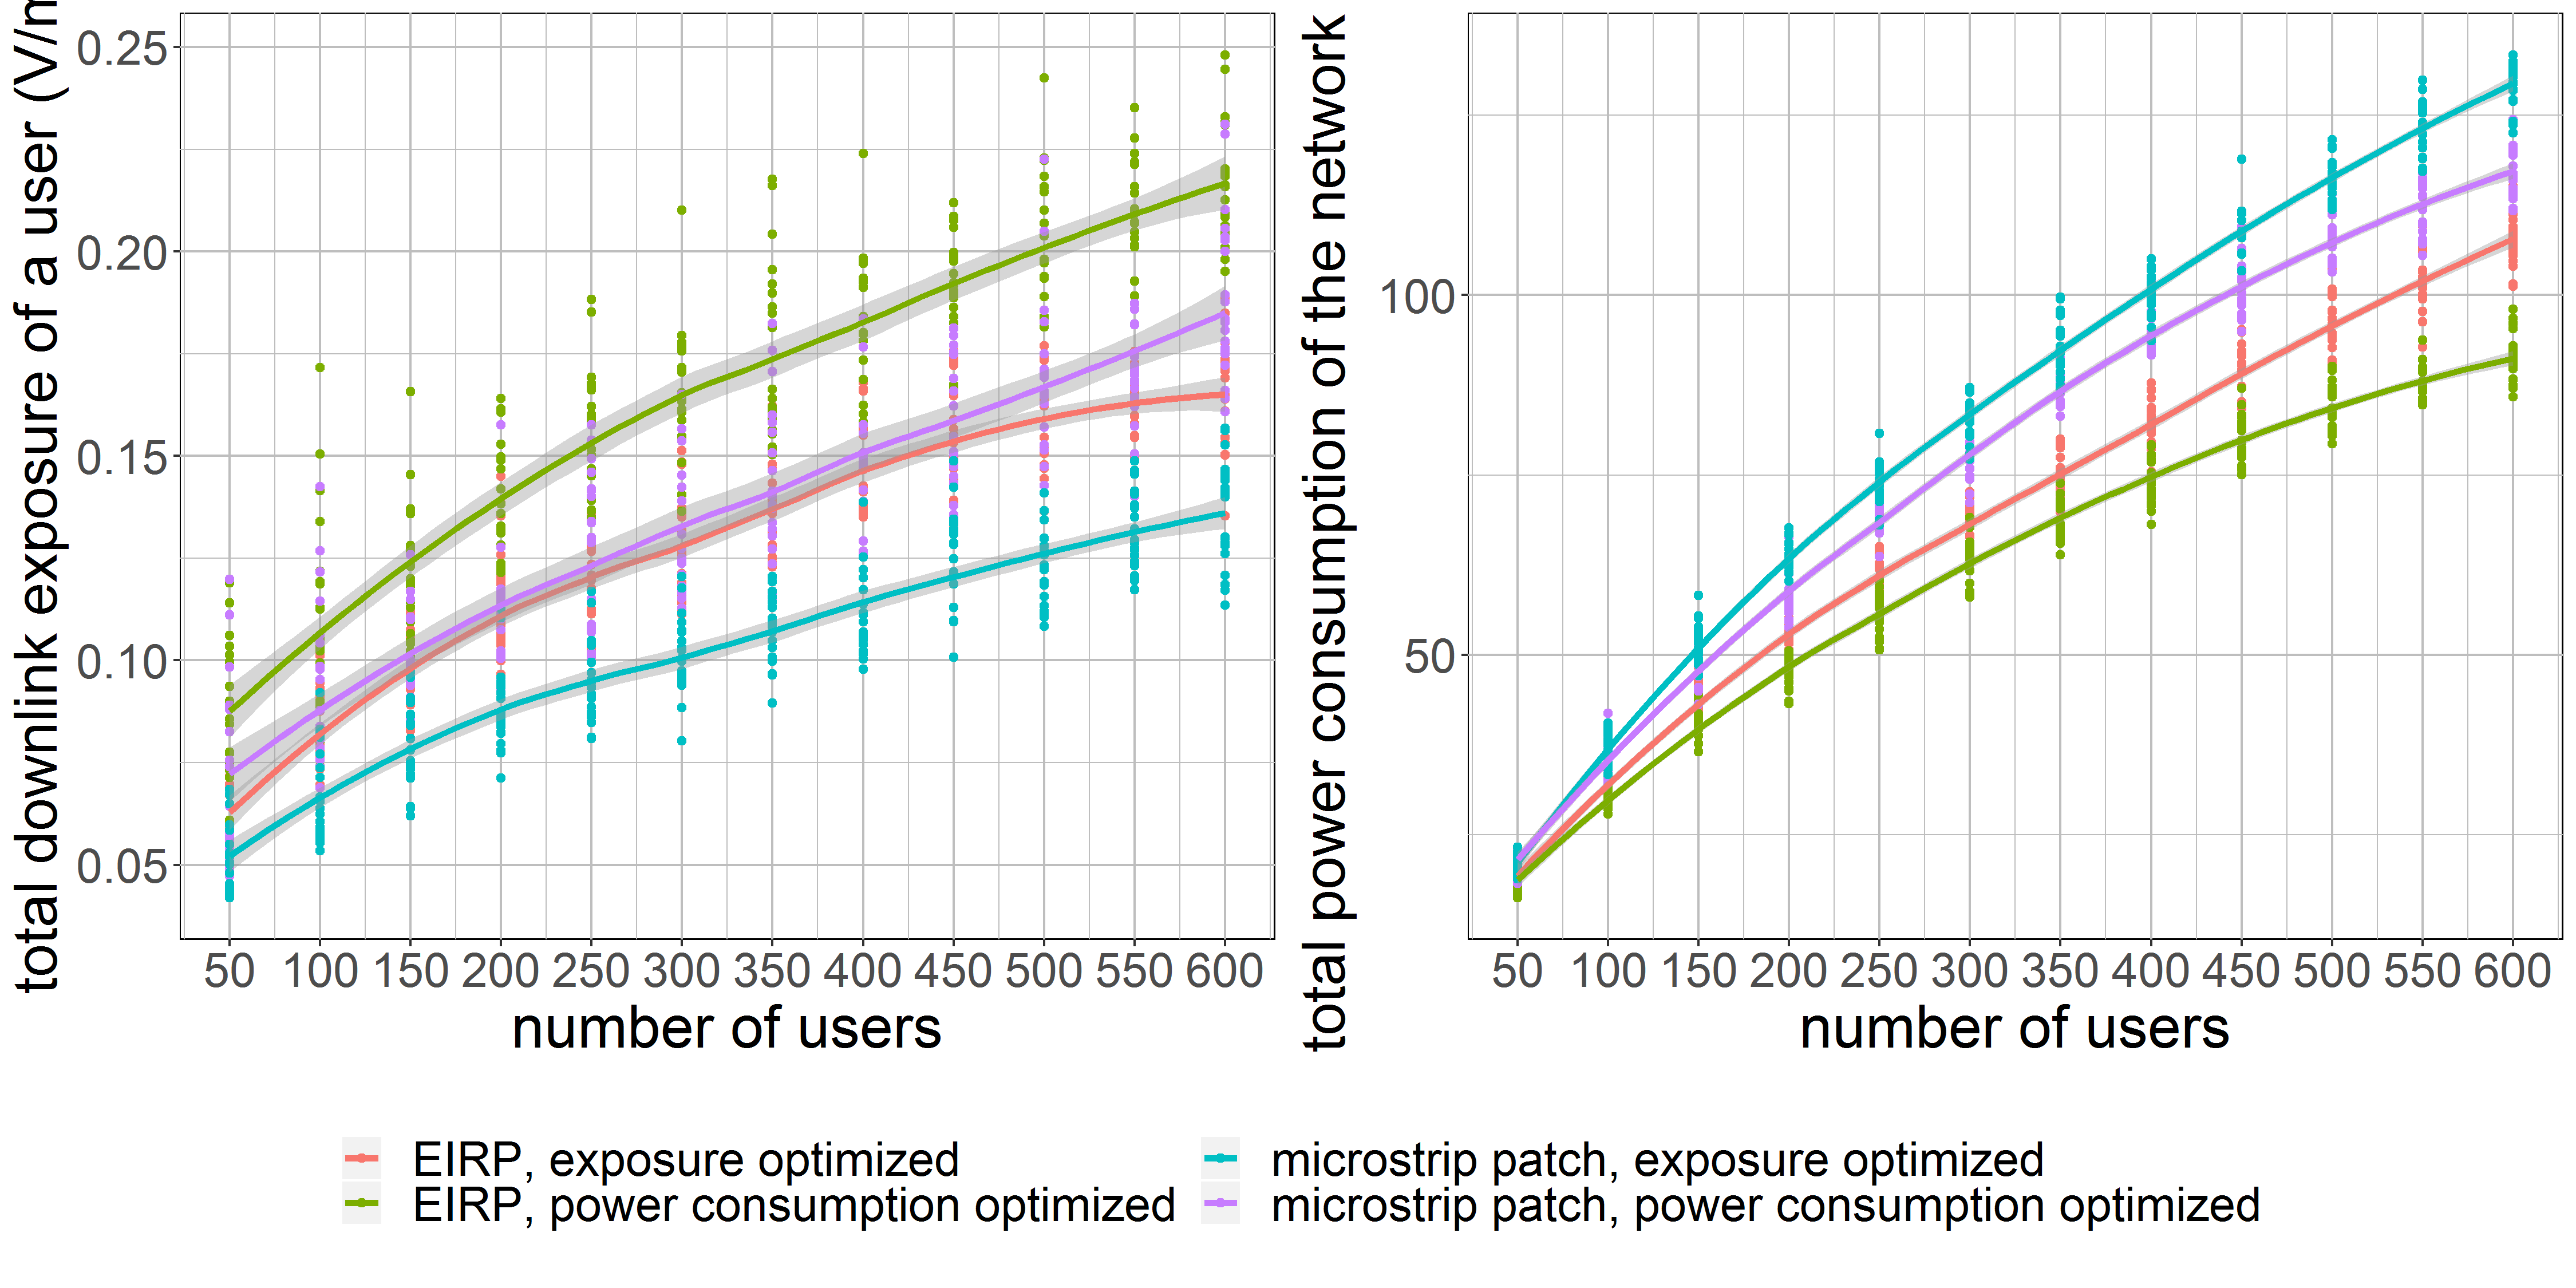
\includegraphics[width=\linewidth]{../results/s3/uvsdlAndPc.png}
  \caption{The influence of the population size on the downlink electromagnetic radiation (a) and power consumption (b).}
  \label{fig:s3b_dlAndPC}
%\bigbreak
 % 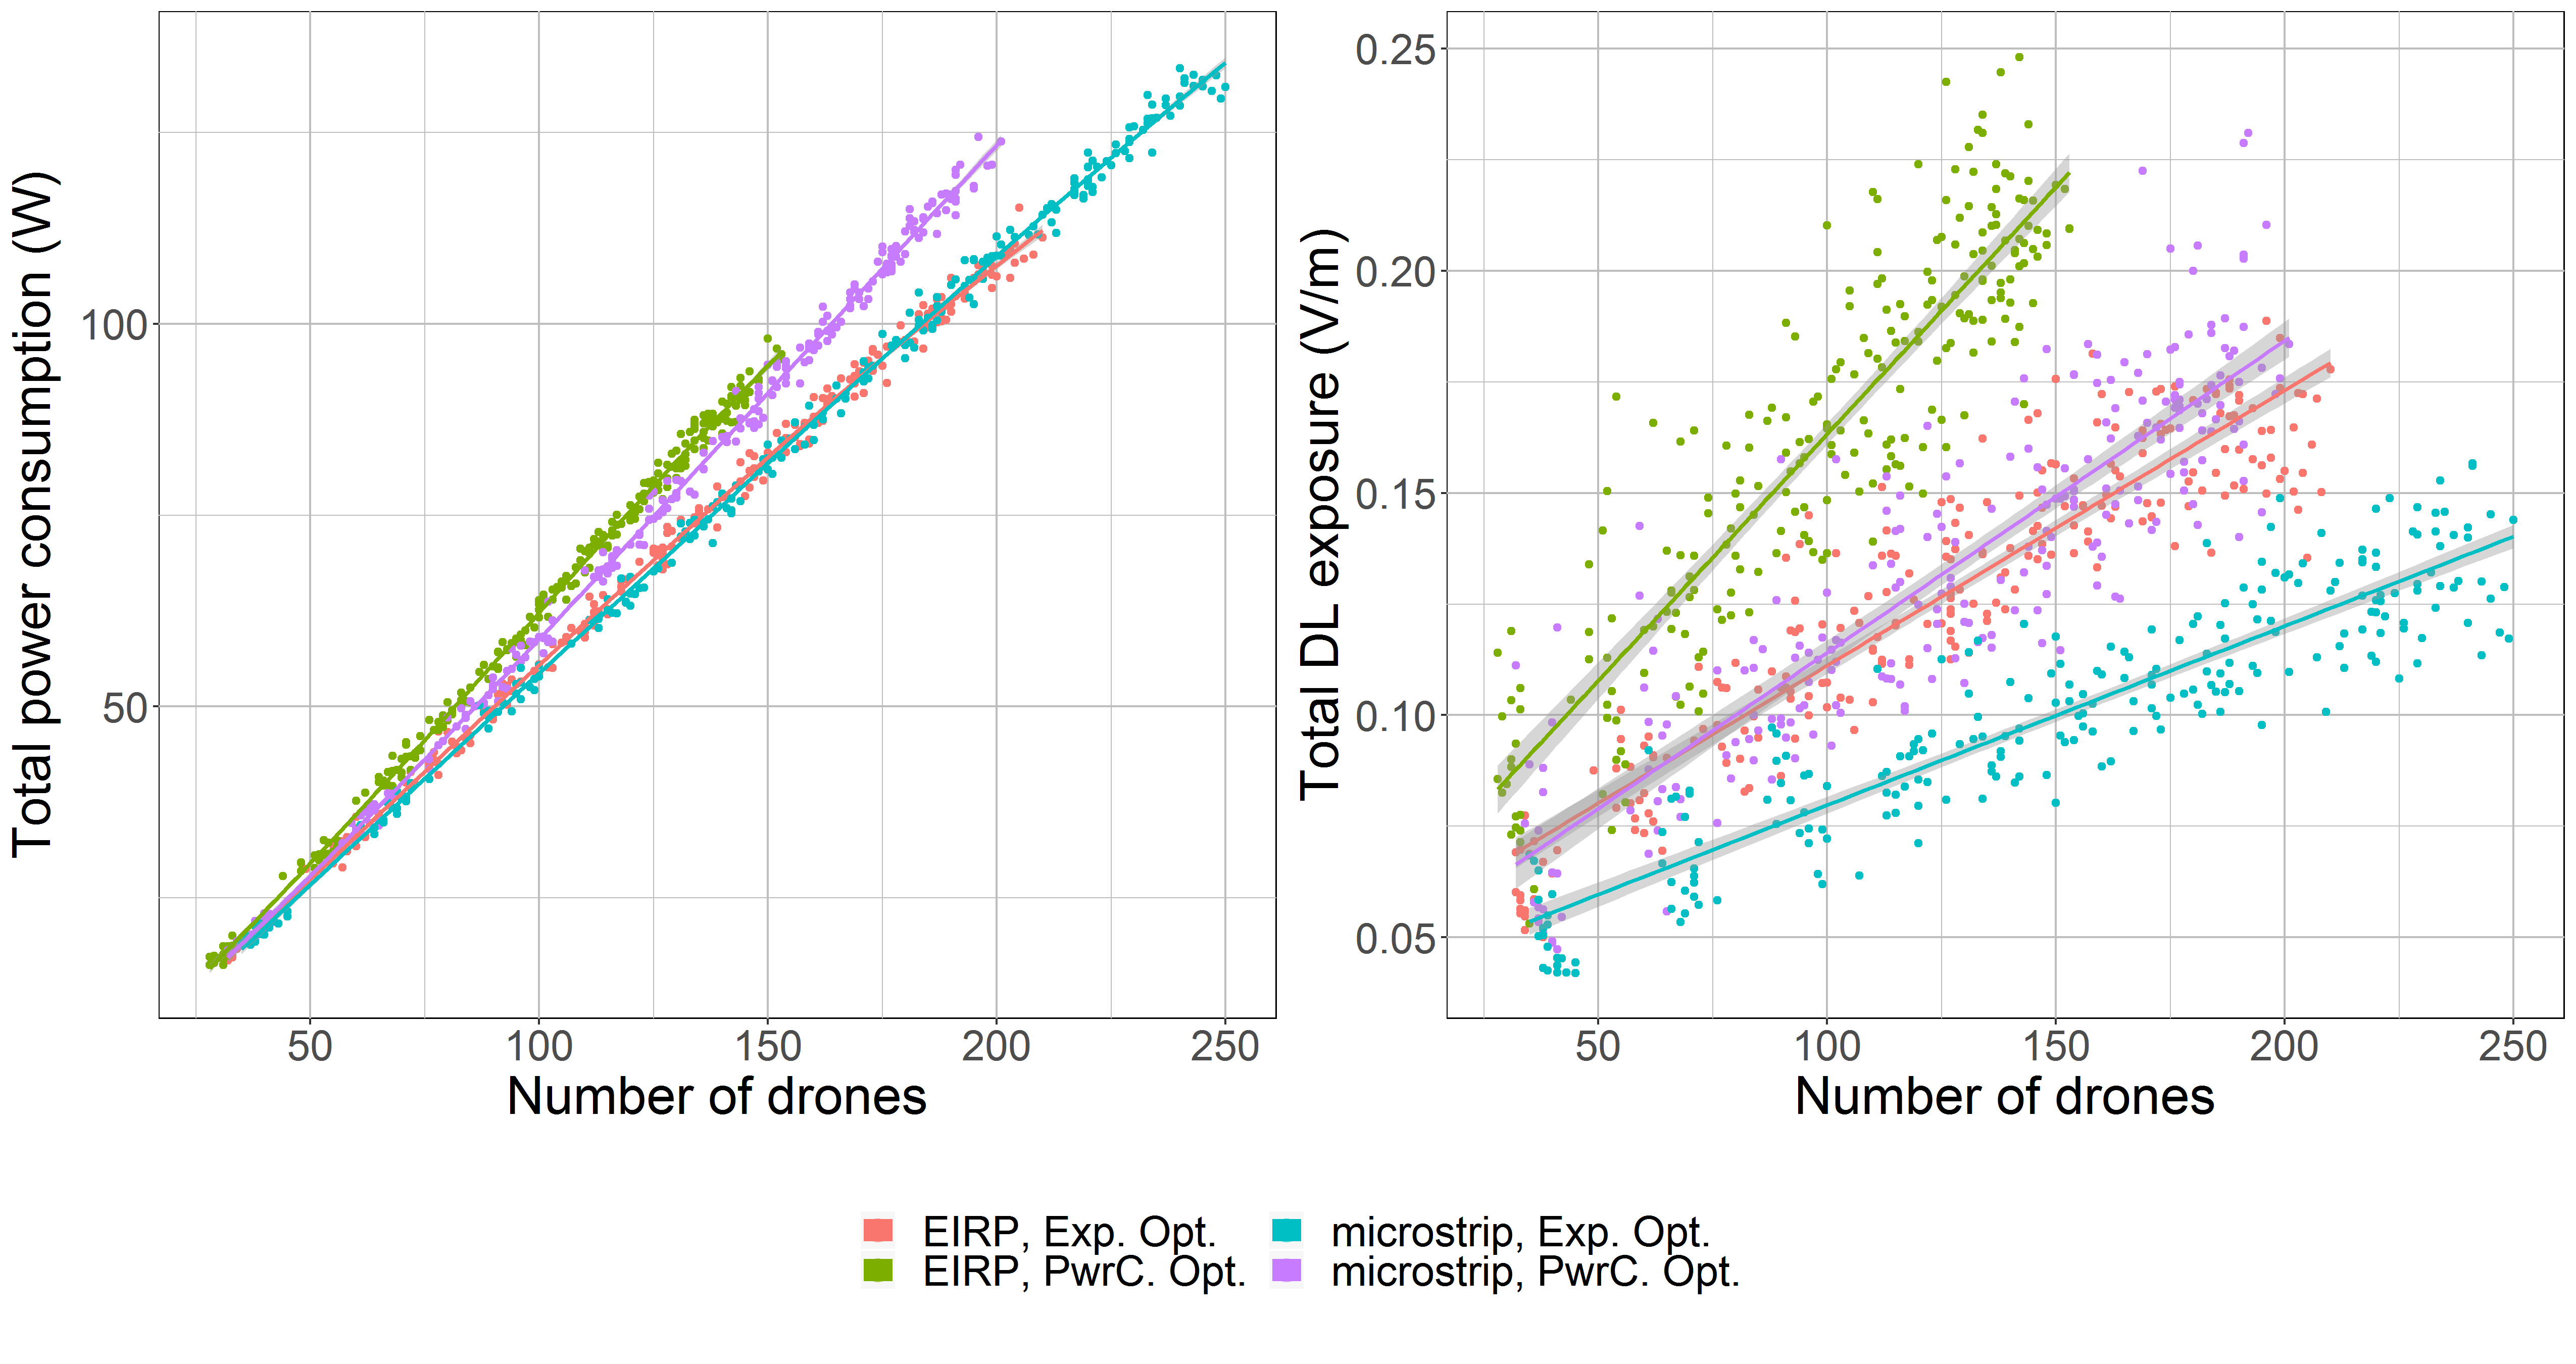
\includegraphics[width=\linewidth]{../results/s3/u_numdronesvsdlAndPc.png}
  %\caption{The influence of the number of UABSs on the downlink electromagnetic radiation (a) and power consumption (b).}
  %\label{fig:s3b_dlAndPC2}
\end{figure}

Figure \ref{fig:s3b_fourSourcesMatrix} represents the 
\gls{SAR} from the weighted average user and shows how the \gls{SAR} coming from the user's own device remains almost constant. 
The flying altitude is always the same so 
also the required energy to cover that distance will remain the same. 
For both optimization strategies, the $SAR^{myUE}$ for networks with \gls{isotropicradiator}s vary around $1.1\ \mu W/kg$  %between 1 $\mu W/kg$ and 1.2 $\mu W/kg$ 
 and around  0.7 $\mu W/kg$ for networks using microstrip patch antennae.
The $SAR^{myUABS}$ barely increases in an exposure optimized network and is situated around 0.5 $\mu W/kg$ for both antennae.
The power consumption optimized network also starts around 0.5 $\mu W/kg$ but increases when more users become online. 
A normal behaviour when considering that these \gls{UABS}s try to cover much more users. Therefore, the $SAR^{myUABS}$ 
with 600 users increases up to 1 $\mu W/kg$ for an \gls{isotropicradiator} and almost 2 $\mu W/kg$ for a microstrip patch antenna.
The \gls{SAR} value that increases the most is $SAR^{otherUABS}$ which 
starts really low with less than 0.1 $\mu W/kg$ for 50 users for all configurations. 
The \gls{SAR} increases however very fast. The biggest increase is noticed in an \gls{EIRP} \gls{PwrC Opt} network 
where 3 $\mu W/kg$ is measured for 600 users. The $SAR^{otherUE}$ increases the least for microstrip \gls{Exp Opt} with 
only 1 $\mu W/kg$ for 600 users.
\begin{figure}[h!]
  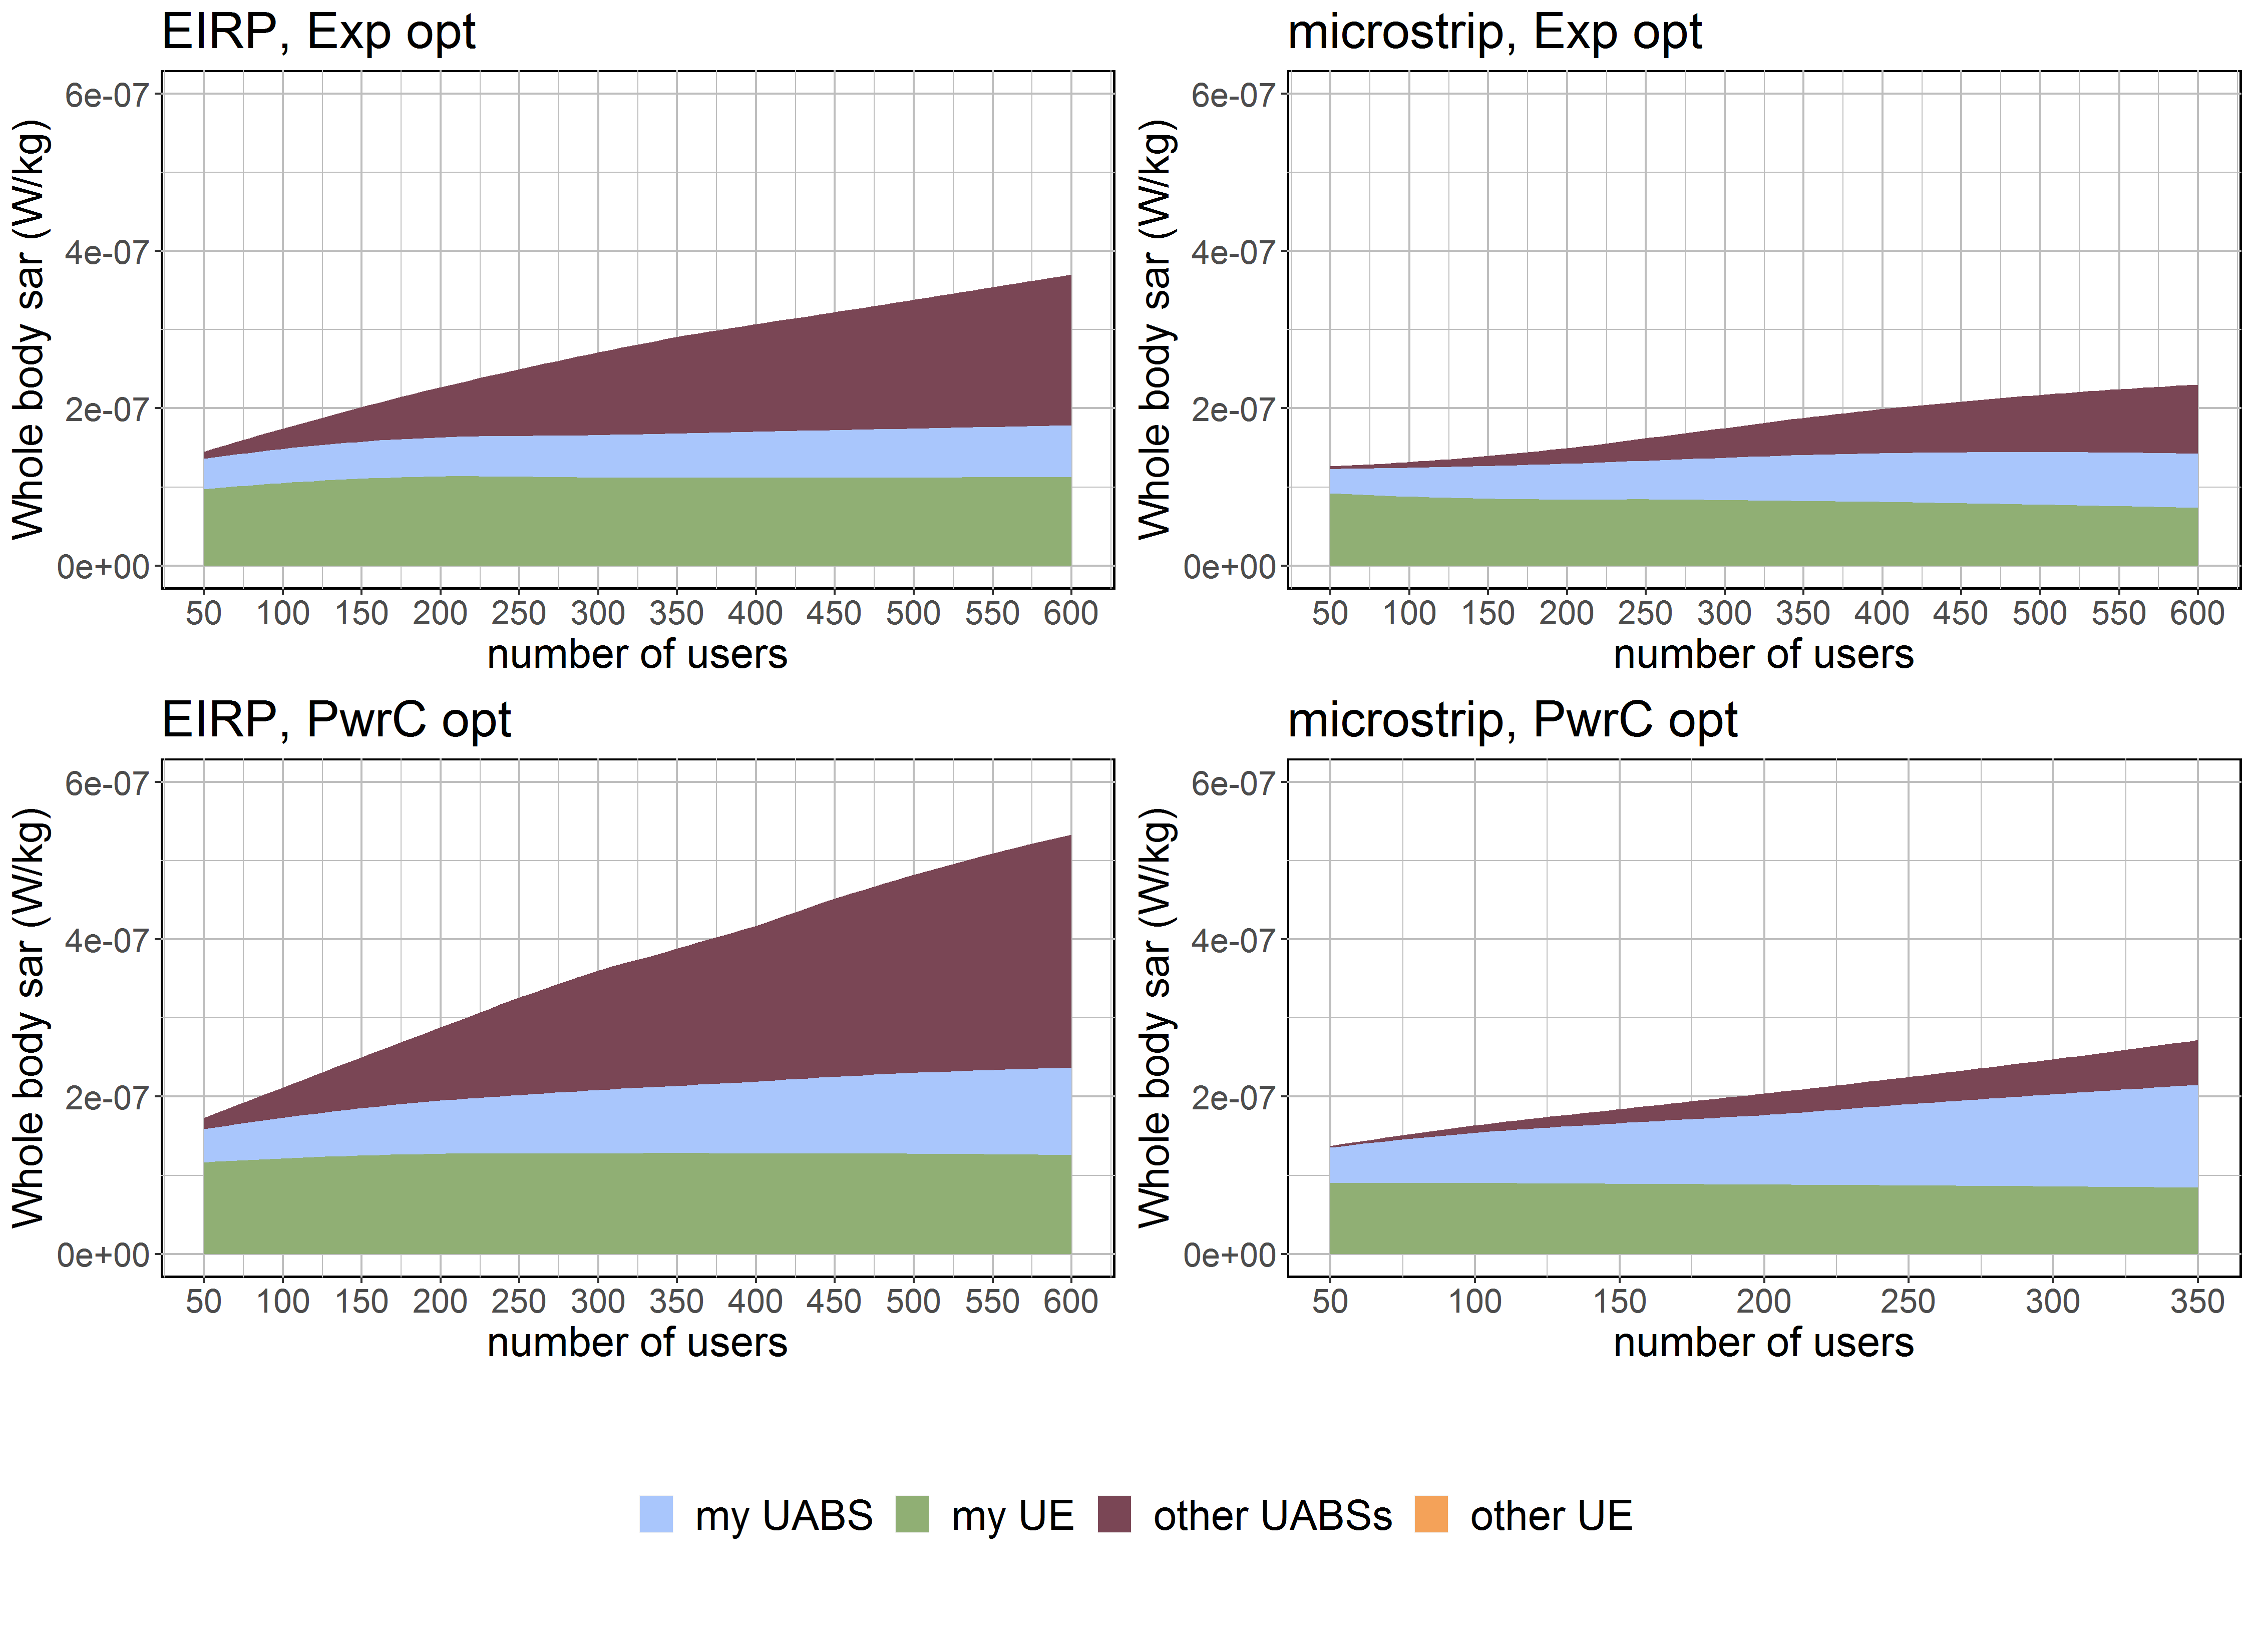
\includegraphics[width=\linewidth]{../results/s3/uFourSources.png}
  \caption{Each figure corresponds with a certain configuration and shows how the \acs{SAR} 
  from different sources are influenced by an increasing population size. An unlimited number of \acs{UABS}s is available.
}
  \label{fig:s3b_fourSourcesMatrix}
\end{figure}

\section{Conclusion}

A capacity-based deployment tool has been used to identify the \gls{SAR} of a user and how a network can be optimized 
towards \gls{DL} electromagnetic exposure and overall power consumption. This has been investigated for different flying heights,
number of users and number of available \gls{UABS}s.
The  results confirm that optimizing towards electromagnetic exposure and total power consumption indeed result in 
conflicting requirements as it was already stated in  \cite{J1}. The proposed fitness function works as intended. 
For default networks, the electromagnetic field radiation from a
power consumption optimized network can be reduced up to 23\% for \gls{isotropicradiator}s and 30\% for microstrip patch antennae 
by optimizing towards electromagnetic exposure. Doing so, decreases the range of the \gls{UABS} and much more \gls{UABS}s will be needed. 
Therefore, exposure optimized networks will, on average, use 18 \gls{UAV}s more than power consumption optimized networks
and require therefore 5 $W$ more energy.

%	How does the network behave differently after the introduction of a realistic antenna?
A directional microstrip patch antenna is introduced because it gives several advantages compared to omnidirectional antennae.
Directional antennae are able to focus their energy there where it is needed, namely towards the ground. Microstrip patch antennae 
further benefit from their thin and lightweight design. 
A microstrip patch antenna with an aperture  angle of \ang{90} causes less electromagnetic exposure and coverage and requires more power compared to an \gls{isotropicradiator}.
For a default network, a microstrip patch antenna can reduce between 30\% and 34\% of the electromagnetic exposure 
emitted by an \gls{isotropicradiator}. This will increase the power consumption with 11 $W$.
\begin{figure}[hb!]
\centering
  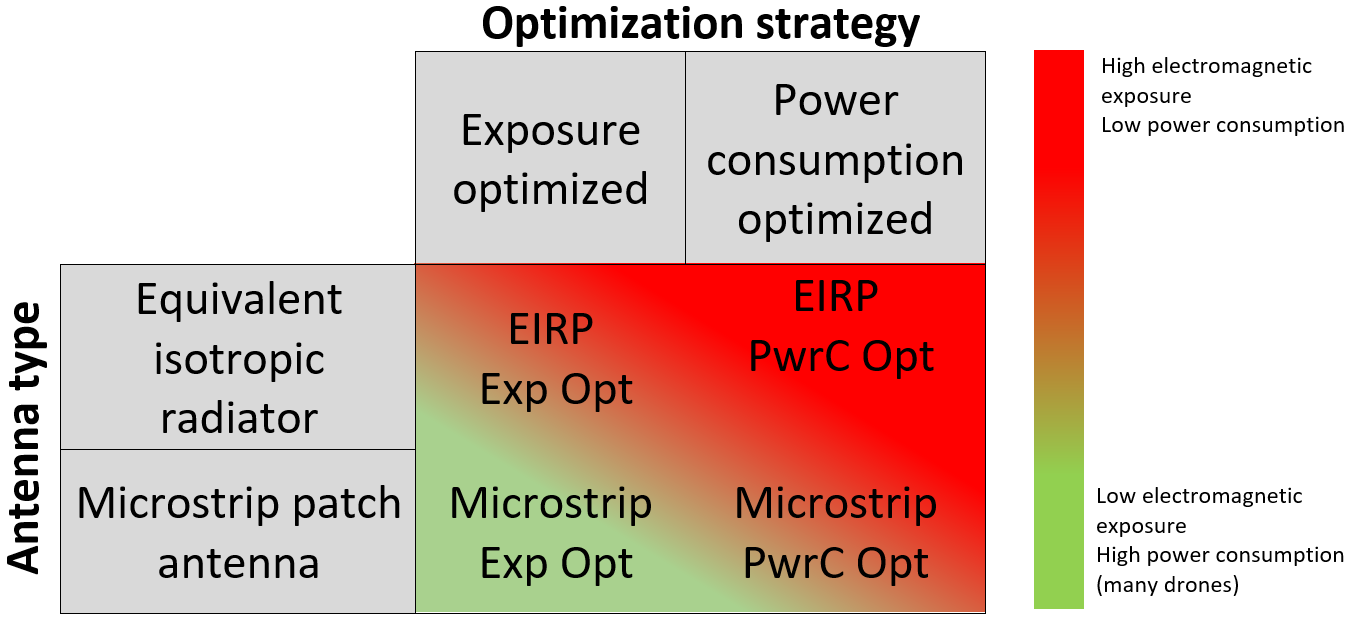
\includegraphics[width=0.8\linewidth]{../images/fourCasesMatrixSol.png}
  \caption{Matrix with the four possible configurations, colour-coded based on the results.}
  \label{fig:resultIllustration}
\end{figure}

Figure \ref{fig:resultIllustration} shows an overview based on the results from the two optimization strategies and the two types of antenna.
Remarkable is that an \gls{EIRP} exposure optimized network behaves very similar to a microstrip power consumption optimized network.
Therefore, the microstrip patch antenna in a power consumption optimized network is recommended. 
The microstrip patch antenna will generate less electromagnetic radiation by design and
the power consumption optimization reduces the number of required \gls{UAV}s and power. A microstrip patch antenna with an aperture 
angle of \ang{90} is considered as a good solution but if budget is more limited, an antenna with a larger aperture angle 
would further reduce cost without interfering with the Flemish legislation regarding electromagnetic exposure.
The \gls{SAR} from the configuration with the most exposure is still a hundred thousandth of the maximal allowed whole body \gls{SAR}.


%What is the contribution of each source towards the total electromagnetic exposure?
Figure \ref{fig:pie} gives
an overview of the contribution of \gls{SAR} in percentage to the total 
exposure for a default network. The values have been averaged over all four considered configurations. 
The user's main source of exposure is clearly the user's own device which contributes 52\% of the total experienced exposure.
A conclusion that was also made by the authors of \cite{J17_kuehn2019modelling} and  \cite{J10.1.1}.
Further, in \cite{J10.1.1} is also concluded that,
thanks to power control, the electromagnetic radiation from the mobile phone 
comes really close to the exposure from the \gls{UABS}. 
Also this is confirmed by the results. Figure \ref{fig:pie} shows that the electromagnetic exposure 
from all \gls{UABS}s together covers the remaining 48\% of which 15\% is from the serving UABS. 
The electromagnetic
 exposure from devices belonging to other people can be ignored compared to the much higher electromagnetic exposure from the other sources
 and contributes only 0.0001\%. It is important to notice that a rather low \gls{pusch} value is used in equation \ref{eq:powerUE} for determining the 
 \gls{UL} radiation and it is believed that a higher value will have a major effect on the \gls{SAR} from the user's own 
 device but also from neighbouring devices.

\definecolor{c_myuabs}{HTML}{A9C6FC}
\definecolor{c_otheruabs}{HTML}{7A4655}
\definecolor{c_myue}{HTML}{90AF74}
\definecolor{c_otherue}{HTML}{F4A259}

\def\angle{0}
\def\radius{3}
\def\cyclelist{{"c_myue","c_otheruabs","c_myuabs","c_otherue"}}
\newcount\cyclecount \cyclecount=-1
\newcount\ind \ind=-1
\begin{figure}
\centering
 \resizebox {!} {4cm} {
\begin{tikzpicture}[nodes = {font=\sffamily}]
  \foreach \percent/\name in {
      52/ my UE,
      33/ other UABSs,
      15/ my UABS,
      0/ Other UE
    } {
      \ifx\percent\empty\else               % If \percent is empty, do nothing
        \global\advance\cyclecount by 1     % Advance cyclecount
        \global\advance\ind by 1            % Advance list index
        \ifnum3<\cyclecount                 % If cyclecount is larger than list
          \global\cyclecount=0              %   reset cyclecount and
          \global\ind=0                     %   reset list index
        \fi
        \pgfmathparse{\cyclelist[\the\ind]} % Get color from cycle list
        \edef\color{\pgfmathresult}         %   and store as \color
        % Draw angle and set labels
        \draw[fill={\color!50},draw={\color}] (0,0) -- (\angle:\radius)
          arc (\angle:\angle+\percent*3.6:\radius) -- cycle;
        \node at (\angle+0.5*\percent*3.6:0.7*\radius) {\percent\,\%};
        \node[pin=\angle+0.5*\percent*3.6:\name]
          at (\angle+0.5*\percent*3.6:\radius) {};
        \pgfmathparse{\angle+\percent*3.6}  % Advance angle
        \xdef\angle{\pgfmathresult}         %   and store in \angle
      \fi
    };
\end{tikzpicture}
 }
\caption{Contribution from each source towards the total SAR that is experienced by the weighted average user. 
The percentages are averaged over the four 
considered configurations.}
\label{fig:pie}
\end{figure}

%How does the \gls{UABS} flying height and number of users influence electromagnetic exposure and power consumption?
Further, the results show that power 
consumption and electromagnetic exposure increases when more users needs to be covered.
When the population increases from 50 to 600 users, 
the electromagnetic radiation increases between 80 and 130 $mV/m$ depending
on the configuration. The power consumption increases with 110 $W$ for all configurations. 
The main source that is influenced by the number of users is the \gls{SAR} from other UABSs with an increase between 1 and 3 $\mu W/kg$, depending on 
the configuration.
Further, increasing the flying altitude has a positive influence on the number of required \gls{UAV}s which on their 
turn have a positive influence on power consumption. Increasing the flying altitude from 20 m to 200 m, decreases the number 
of required \gls{UAV}s around 59\%. This decrease was also noticed in \cite{J2}.
Also authors from \cite{J17_kuehn2019modelling} made the conclusion that reduced path loss decreases electromagnetic exposure.
The electromagnetic radiation from the \gls{UABS}s remains more or less the same for flying altitudes between 80 and 200 metres. Most 
\gls{UABS}s are in \gls{LOS} and no more power will be used thanks to power control.
However, the electromagnetic radiation from the user's own device does increase in order to reach the high flying \gls{UAV}s.
Around 80 metres, the exposure from the  user's device surpasses the exposure from the serving \gls{UABS}.
When more \gls{UABS}s are available in the network, electromagnetic exposure from other \gls{UABS} will increase as well.
This is because more \gls{UABS}s come into \gls{LOS} when the flying height becomes larger. Raising the flying altitude from 20 to 200 m will increase the \gls{SAR} from other 
\gls{UABS}s between 46 and 49 times when using an \gls{isotropicradiator} antenna and between 70 and 85 times when using a microstrip patch antenna.
When also considering the results from \cite{U1} where a flying altitude of  
80 metres is suggested for an optimal access and backhaul connectivity, a flying height 
of 80 metres is also here proposed for the city centre of Ghent.

In conclusion, a microstrip patch antenna with an aperture angle of \ang{90} is a suitable starting point for an antenna. 
This directional antenna focusses electromagnetic radiation where it is needed and unwanted sideways radiation 
is reduced by design.
The sufficiently large aperture angle covers enough users. The antenna is recommended to be deployed in a power consumption 
optimized network since less \gls{UAV}s are required and therefore also less expensive.
The optimal flying height for the city centre of Ghent is believed to be situated at 80 metres since lower flying heights require much more \gls{UABS}s and
higher flying heights have a negative influence on the electromagnetic exposure.  

As a future work, still some parameters require further evaluation. Different \gls{pusch} values
are expected to have a big influence on \gls{UL} radiation and exposure from 
backhaul connections still have to be considered. Further, MiMo and massive MiMo are ready to be supported since 
the tool can easily be extended with some more complex radiation patters 
like  beamforming. Another consideration is improving the time complexity by 
replacing the exact algorithm with an heuristic algorithm. 
 
\section*{Acknowledgement}
Special thanks to the WAVES research group at Ghent University for providing 
access to their capacity based deployment tool and therefore making this research possible.

\bibliographystyle{ieeetr}
\bibliography{referenties}


\end{document}
